\section{Wprowadzenie}

Pomiar poziomu ubóstwa powinien obejmować co najmniej dwa wymiary: jego zasięg oraz głębokość. Z kolei zgodnie z oczekiwaniami użytkowników danych, informacje te powinny być dostarczane dla jak najmniejszych jednostek administracyjnych czy terytorialnych. Stąd też w niniejszym rozdziale podjęto próbę oszacowania stopy oraz głębokości ubóstwa na poziomie podregionów i~powiatów. Wskazano na możliwość wykorzystania w tym celu  metod estymacji scharakteryzowanych w rozdziale trzecim przy użyciu istniejących już źródeł danych w roli tak zwanych \textit{zmiennych pomocniczych} (por. rozdział 2). Rozdział podzielony jest na dwie części. Pierwsza z~nich obejmuje charakterystykę źródeł danych stanowiących podstawę przeprowadzonego badania empirycznego.

Dokonano w niej oceny jakości danych jednostkowych pochodzących z Europejskiego Badania Dochodów i Warunków Życia (EU-SILC) 2011. Szczegółowo została przedstawiona procedura uzyskiwania wektora dochodów ekwiwalentnych w badaniu EU-SILC, który stanowi podstawę szacowania stopy oraz głębokości ubóstwa. Z wykorzystaniem analizy częstości przeanalizowano sposób udzielania odpowiedzi --- wywiad bezpośredni/wywiad zastępczy/imputacja masowa --- oraz skalę imputacji w poszczególnych składowych dochodu reprezentantów badania. Przeprowadzona analiza jest związana ze zjawiskiem wzrastającej niechęci do udziału w prowadzonych badaniach reprezentacyjnych. Wskaźnik braku realizacji wywiadu w przypadku badania EU-SILC w 2006 roku wynosił 48\%, a w roku 2014 już 63\% \citep{dezagregacja2015}.

W drugiej części rozdziału skoncentrowano się na estymacji pośredniej dwóch wskaźników ubóstwa --- stopy oraz głębokości w domenach nieplanowych na etapie projektowania badania. Rok 2011 był ostatnim, w którym Główny Urząd Statystyczny opublikował stopę ubóstwa w~przekroju województw. Z kolei głębokość ubóstwa nie jest w ogóle publikowana w ujęciu przestrzennym. W związku z tym, została podjęta próba estymacji wyżej wymienionych wskaźników na poziomie podregionów oraz powiatów. W tym celu zostaną wykorzystane dwa rodzaje podejść bazujących na modelu: obszarowe oraz jednostkowe. W pierwszej kolejności został zastosowany klasyczny model Faya-Herriota \citep{fh1979} oraz jego rozszerzenie o korelacje przestrzenne \citep{pratesi2008}. Metoda M-kwantylowa (MQ) \citep{mq2006} oraz empiryczna bayesowska (EB) \citep{ebp2010} stanowią rdzeń podejścia jednostkowego --- pierwsza z nich wykorzystuje regresję m-kwantylową, druga natomiast liniowy model mieszany. 

Przedmiotem rozważań był także wpływ transformacji estymowanej cechy na jakość oszacowań. W przypadku modeli obszarowych przeanalizowano przekształcenie wykorzystujące pierwiastek arcus sinusa \citep{analpovdata52016}. To przekształcenie ma na celu stabilizacje wariancji oraz zapewnienie oszacowań z przedziału $[0,1]$. Z kolei w podejściu jednostkowym, w którym zmienną zależną jest dochód gospodarstwa, wykorzystano transformację logarytmiczną, logarytmiczną z~przesunięciem oraz Boxa-Coxa.

\section{Charakterystyka i ocena wykorzystanych źródeł danych}

Europejskie Badanie Dochodów i Warunków Życia, zaprezentowane w rozdziale drugim, jest badaniem dobrze udokumentowanym. Opis założeń oraz szczegółowy wykaz wszystkich zmiennych obejmuje ponad 400 stron \citep{silc2011}. Niemniej jednak podczas szczegółowych analiz natrafiono na pewne problemowe obszary, które zostaną zaprezentowane w tej części pracy. Dotyczy to przede wszystkim sposobu odpowiedzi oraz imputacji wartości dochodu.

Podstawą przeprowadzonych analiz były zanomizowane jednostkowe zbiory danych zebrane podczas realizacji Europejskiego Badania Dochodów i Warunków Życia w 2011 roku. Dostarczona struktura plików jest następująca:

\begin{itemize}
\item plik D - rejestr gospodarstw (12871 obserwacji, 22 cechy),
\item plik R - rejestr osób (36720 obserwacji, 52 cechy),
\item plik H - dane gospodarstw (12871 obserwacji, 205 cech),
\item plik P - dane osób (30421 obserwacji, 308 cech).
\end{itemize}

Wyżej wymienione zbiory można ze sobą połączyć z wykorzystaniem wspólnego klucza jakim jest identyfikator gospodarstwa i osoby. Różnica liczby obserwacji w zbiorach R i P wynika z~faktu, że w badaniu odpowiedzi udzielają tylko osoby w wieku 16 lat i więcej, natomiast rejestr osób zawierał informacje o wszystkich osobach wchodzących w skład gospodarstwa domowego.

\subsection{Sposób przekazywania odpowiedzi w badaniu EU-SILC}

W rejestrze osób znajduje się zmienna przechowująca informację o sposobie przeprowadzenia wywiadu z respondentem (RB260). Przyjmuje ona pięć kategorii - wywiad bezpośredni (metodą PAPI lub CAPI), wywiad telefoniczny, samodzielne wypełnienie przez respondenta oraz wywiad zastępczy. Wywiad zastępczy jest rodzajem wywiadu bezpośredniego, który jest przeprowadzany z osobą reprezentującą respondenta należącą do wylosowanego gospodarstwa domowego.

62\% odpowiedzi udało się pozyskać poprzez wywiad bezpośredni, natomiast 15\% stanowiły dane pochodzące z wywiadu zastępczego. Pozostałe 23\% to braki danych, które miały źródło dwojakiego rodzaju. W pierwszym przypadku osoba zamieszkująca gospodarstwo nie miała ukończonych 16 lat i zgodnie z założeniami badania nie był z nią przeprowadzany wywiad (17\%), natomiast w drugim przypadku dane respondenta zostały uzupełnione z wykorzystaniem ``full-record imputation'' (6\%)\footnote{Dokumentacja badania nie precyzuje co oznacza to określenie, na co zwracają uwagę autorzy artykułu \citep{iacovou2012}. Najpewniej jest to tzw. imputacja masowa wykorzystywana w przypadku braków odpowiedzi, gdzie cały rekord jest imputowany. Ta procedura nie jest jednak opisana.}.

W związku z tym, że odpowiedzi udzielane podczas wywiadu zastępczego pochodzą z tzw. drugiej ręki mogą być obarczone występowaniem błędów nielosowych, wynikających np. z niewiedzy osoby zastępującej. W pracy ocenie poddano skalę występowania wywiadu zastępczego m.in. w przekroju województw oraz według wieku.

\begin{figure}[ht]
\centering
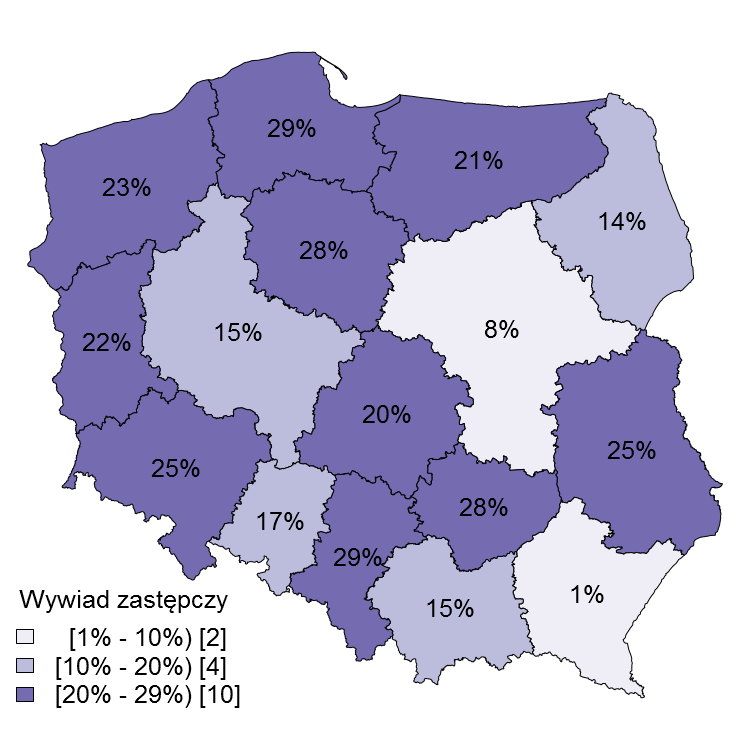
\includegraphics[width=0.6\textwidth]{04_wykresy/wywiad-woj.png}
\caption{Odsetek wywiadów zastępczych w badaniu EU-SILC 2011 w przekroju województw}
\small{Źródło: opracowanie własne na podstawie badania EU-SILC 2011.}
\label{fig:wywiad_woj}
\end{figure}

Rozkład odpowiedzi pochodzących z wywiadu zastępczego charakteryzuje się znacznym przestrzennym zróżnicowaniem (por. rys. \ref{fig:wywiad_woj}). Najwyższy odsetek tak przeprowadzonego wywiadu obserwuje się w województwie pomorskim oraz śląskim --- 29\%. W środkowej grupie z wartościami pomiędzy 14\% a 17\% znalazły się województwa: podlaskie, małopolskie, wielkopolskie oraz opolskie. Województwo mazowieckie charakteryzuje się 8\% udziałem przeprowadzonych wywiadów zastępczych. Z kolei w województwie podkarpackim odnotowano zaledwie 1\% wywiadów zastępczych.

Na rysunku \ref{fig:wywiad_wiek} przedstawiono także występowanie tego zjawiska według roczników wieku.

\begin{figure}[ht]
\centering
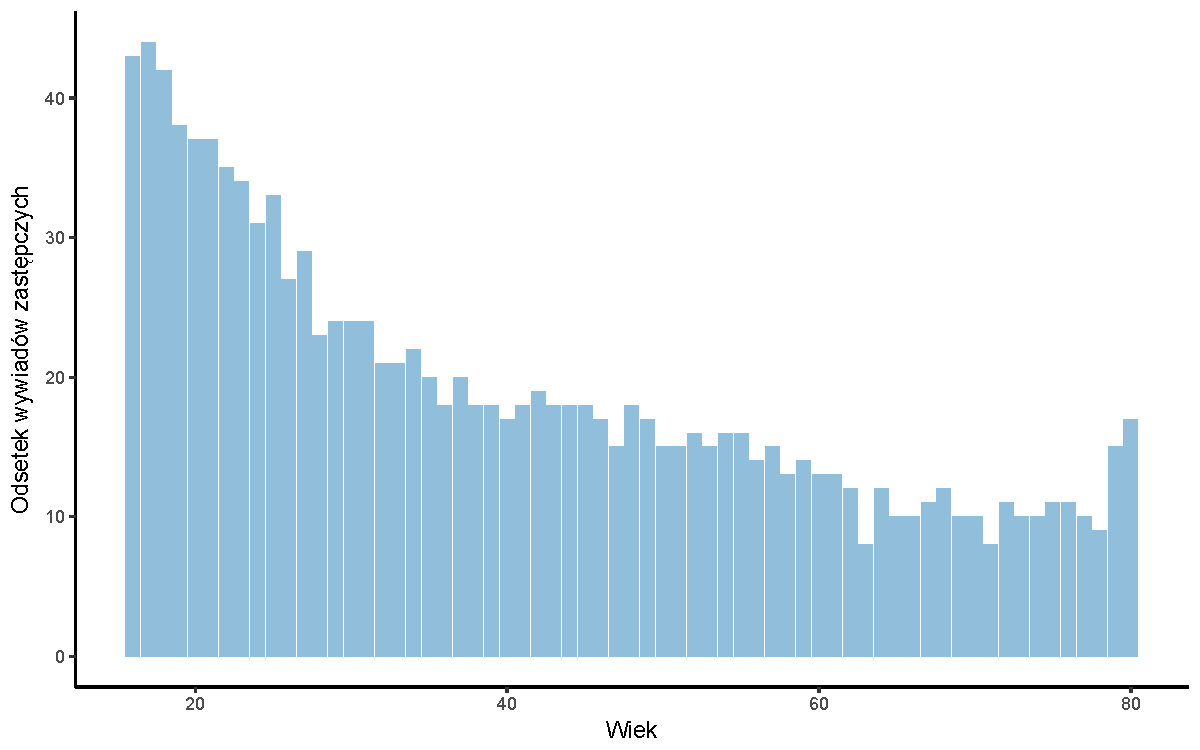
\includegraphics[width=0.8\textwidth]{04_wykresy/sposob_przeprowadzenia_wywiadu_wiek-1.pdf}
\caption{Odsetek wywiadów zastępczych w badaniu EU-SILC według roczników wieku}
\small{Źródło: opracowanie własne na podstawie badania EU-SILC 2011.}
\label{fig:wywiad_wiek}
\end{figure}

Wywiady zastępcze najczęściej były realizowane za osoby w wieku 16, 17 i 18 lat. Można także zaobserwować wyższy udział wywiadów przeprowadzonych w zastępstwie osób w wieku co najmniej 80 lat. Badanie EU-SILC nie wskazuje maksymalnego wieku respondenta, ale w~dostarczonych danych dokonano zgrupowania osób w wieku 80 lat i starszych w~jedną kategorię w~celu zachowania tajemnicy statystycznej \citep{ciani2011}. Niestety, podobnie jak wcześniej, w dokumentacji badania nie ma informacji na ten temat.

\subsection{Analiza struktury cech wykorzystanych w estymacji wskaźników ubóstwa}\label{pr:struktura-zmiennych}

Najistotniejszą z punktu widzenia analizy ubóstwa zmienną jest roczny ekwiwalentny dochód do dyspozycji gospodarstwa. Wyznaczenie tego wektora dochodów polega na zsumowaniu wszystkich składników dochodu gospodarstwa, w tym dochodów poszczególnych osób wchodzących w skład gospodarstwa i pomniejszeniu go o rozchody, czyli przede wszystkim transfery społeczne. Tak wyznaczone wartości przelicza się uwzględniając demograficzny wymiar badanego gospodarstwa z~wykorzystaniem zmodyfikowanej skali ekwiwalentności OECD. Poniżej wymieniono poszczególne składniki składające się na dochód gospodarstwa --- symbol zmiennej w badaniu EU-SILC, pełną nazwę oraz skrót wykorzystywany na rysunkach.

Spośród składników dochodu osób \emph{in plus} wlicza się:

\begin{itemize}
\item PY010G --- dochód pieniężny z pracy najemnej brutto (p.~najemna),
\item PY021G --- wykorzystanie samochodu służbowego do celów prywatnych brutto (samochód),
\item PY050G --- dochód z pracy na własny rachunek brutto (p.~własna),
\item PY080G --- emerytura z indywidualnych funduszy emerytalnych brutto (III filar),
\item PY090G --- świadczenia dla bezrobotnych brutto (św. bezr.),
\item PY100G --- świadczenia związane z wiekiem brutto (św. wiek),
\item PY110G --- renta rodzinna brutto (renta),
\item PY120G --- świadczenia chorobowe brutto (św. chorob.),
\item PY130G --- świadczenia dla niepełnosprawnych brutto (św. niep),
\item PY140G --- stypendia brutto (stypendia).
\end{itemize}

Na poziomie gospodarstwa do dochodu wlicza się:

\begin{itemize}
\item HY040G --- dochód z wynajmu nieruchomości brutto (doch. nieruch.),
\item HY050G --- świadczenia dotyczące rodziny brutto (św. rodz.),
\item HY060G --- świadczenia dotyczące wykluczenia społecznego brutto (św. wykl.),
\item HY070G --- dodatki mieszkaniowe brutto (dod. mieszk.),
\item HY080G --- regularne transfery pieniężne otrzymywane od osób spoza gospodarstwa domowego brutto (transfery),
\item HY090G --- dochód z własności finansowej (kapitałowy) brutto (kapitał),
\item HY110G --- dochód dzieci do lat 16 brutto (doch. dzieci).
\end{itemize}

Na dochód \emph{in minus} wpływają:

\begin{itemize}
\item HY120G --- podatki od nieruchomości brutto (pod. nieruch.),
\item HY130G --- regularne transfery pieniężne przekazywane osobom spoza gospodarstwa domowego brutto (transfery),
\item HY140G --- podatek dochodowy, składki na ubezpieczenie społeczne brutto (pod. doch.).
\end{itemize}

Ponadto każdej zmiennej dochodowej towarzyszy zmienna flagowa, która przechowuje informację o tym czy dana wartość była imputowana i jeśli tak, to w jaki sposób. Według dokumentacji badania, zmienna zawierająca informację o sposobie imputacji powinna być pięciocyfrowa. Wówczas pierwsza cyfra zawiera kategorię dochodu (netto/brutto), druga cyfra to metoda imputacji, natomiast ostatnie trzy cyfry to współczynnik imputacji (iloraz wartości zebranej i zapisanej). W~praktyce poszczególne kraje stosują swoje standardy kodowania tej zmiennej \citep{brandolini2010}. W polskim badaniu EU-SILC na podstawie wartości flagi można wyodrębnić następujące kategorie: 1) kompletna informacja o dochodzie, 2) częściowa informacja o dochodzie oraz 3) brak informacji o dochodzie.

Rysunek \ref{fig:dochod_osoby} przedstawia wartości poszczególnych składników dochodu uzyskiwanych przez osoby zamieszkujące gospodarstwo domowe. Jedna osoba mogła uzyskiwać dochody z kilku źródeł, w związku z czym liczebności wszystkich kategorii nie sumują się do liczby przebadanych respondentów. Z racji bardzo dużych wartości występujących w kategoriach praca najemna oraz praca na własny rachunek ograniczono oś Y do wartości 50 000 zł. 

\begin{figure}[ht]
\centering
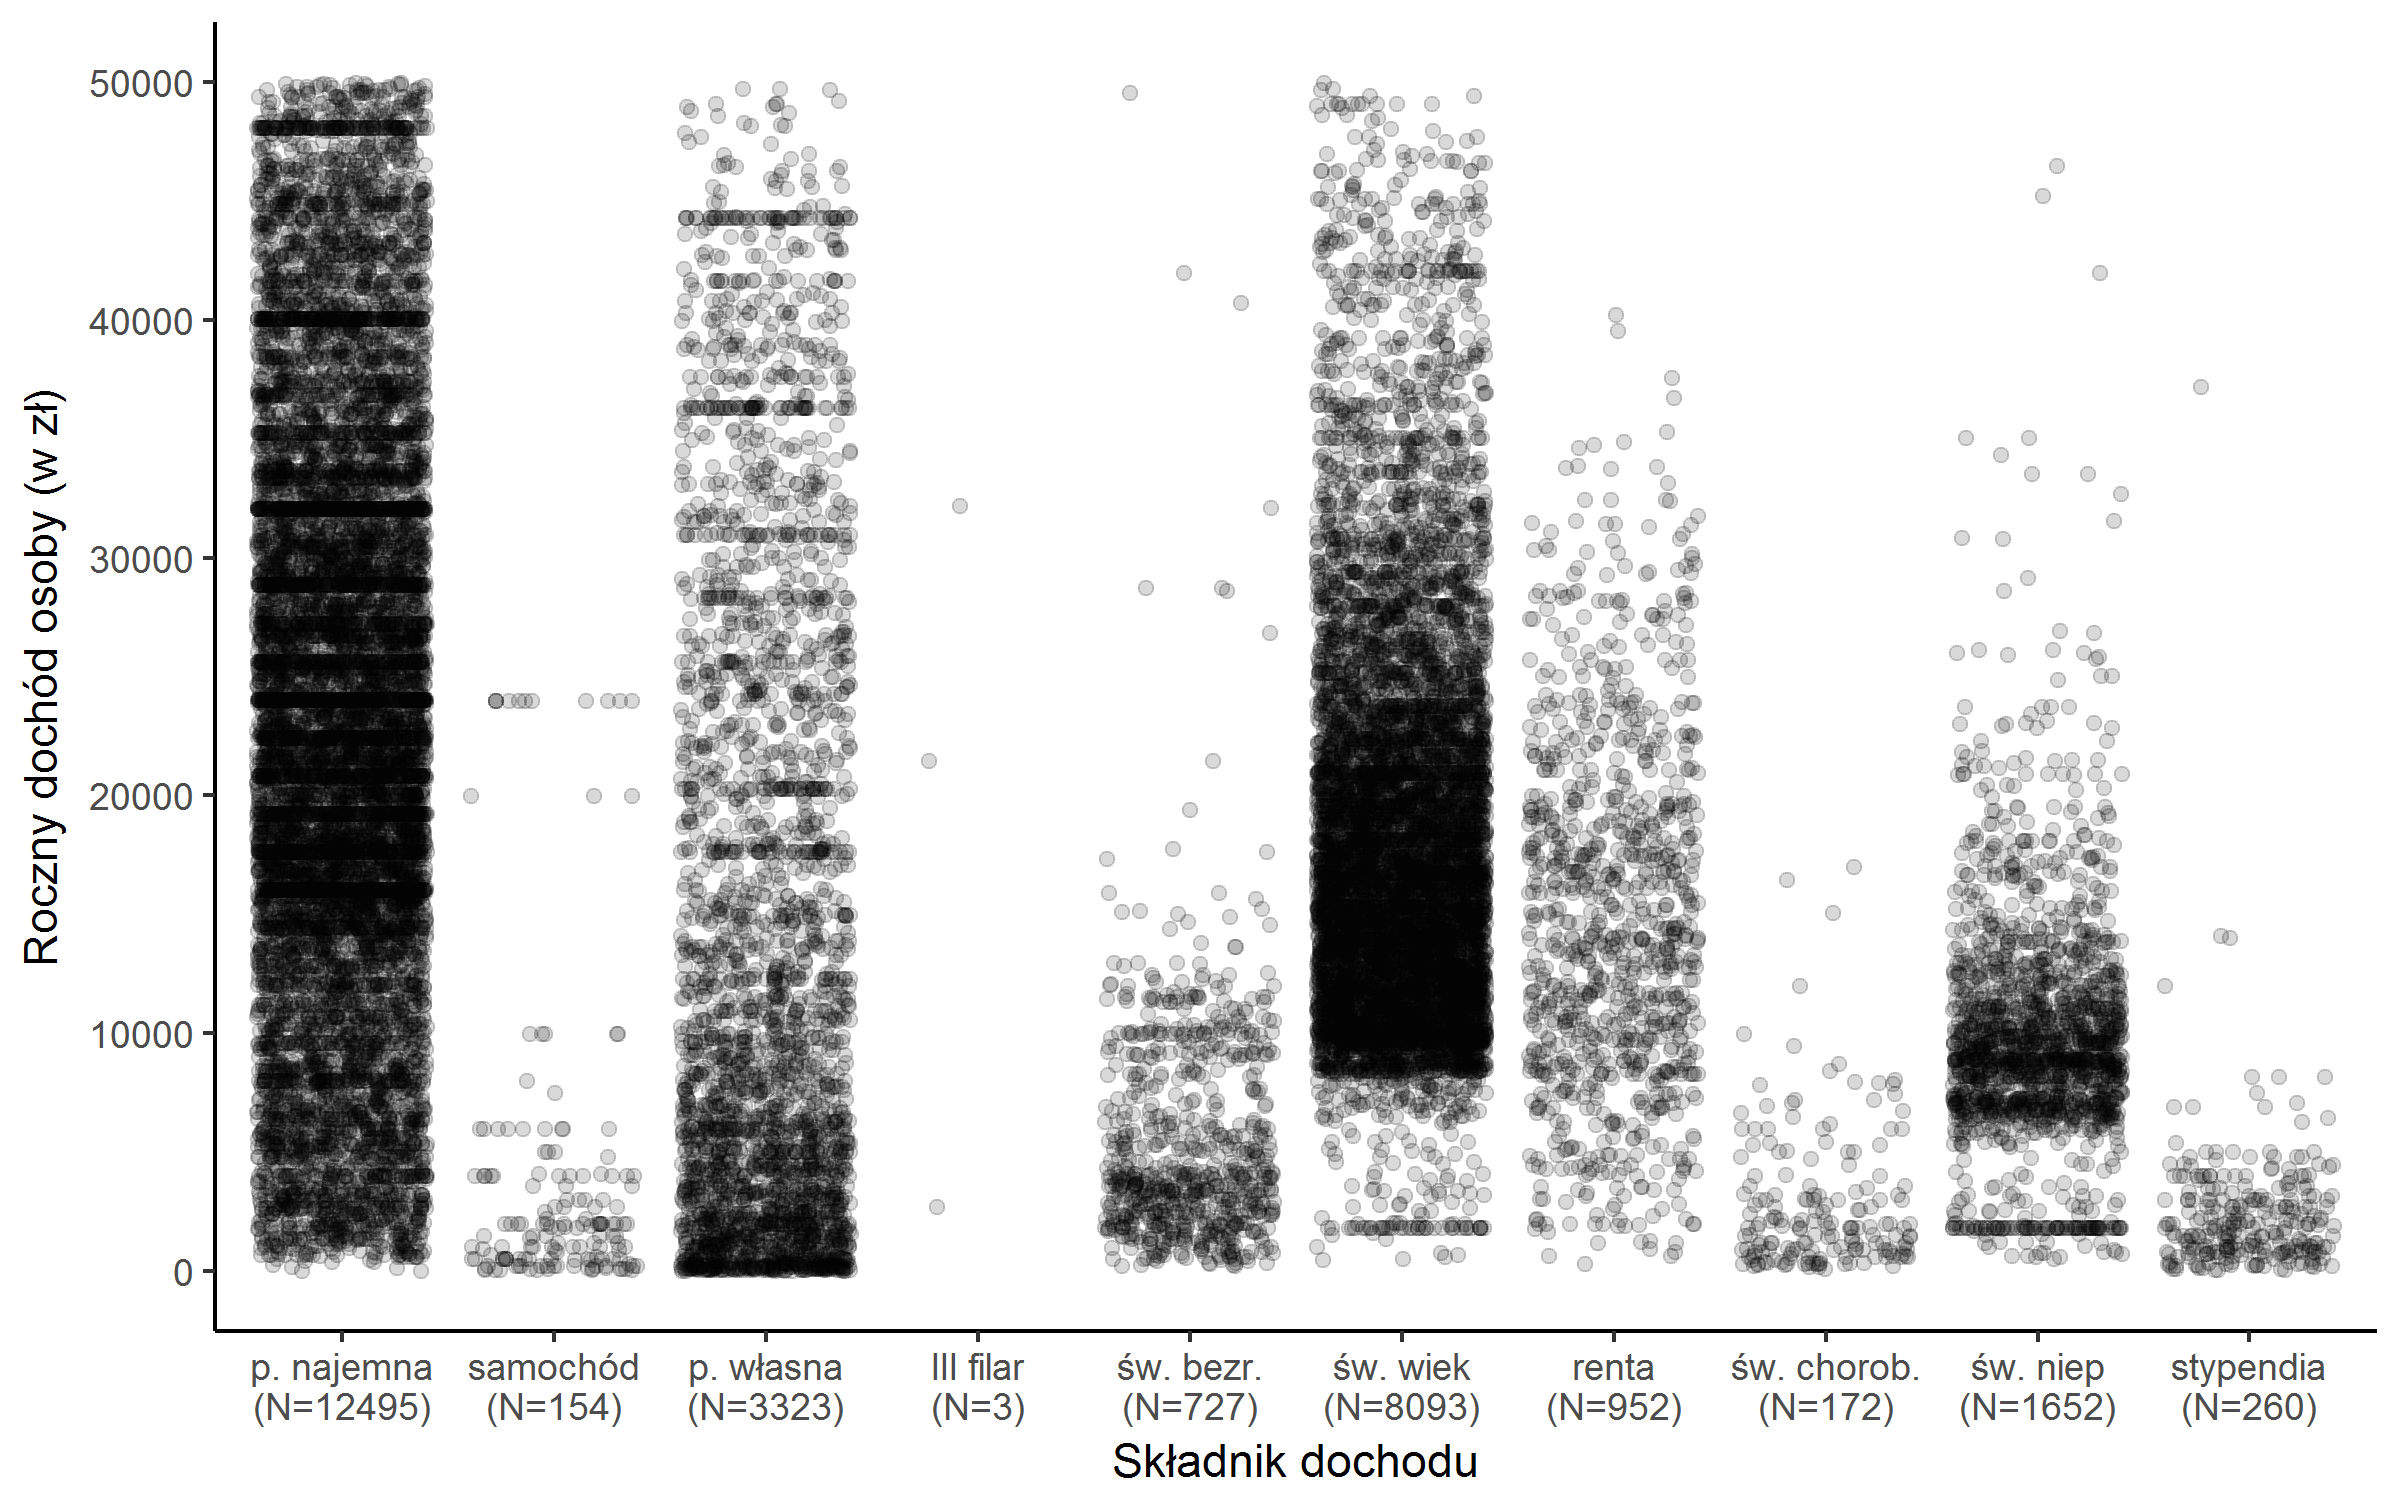
\includegraphics[width=0.8\textwidth]{04_wykresy/dochod_osoby-1.png}
\caption{Wartości dochodu osób w badaniu EU-SILC 2011 według kategorii dochodu (do 50000 zł)}
\small{Źródło: opracowanie własne na podstawie badania EU-SILC 2011.}
\label{fig:dochod_osoby}
\end{figure}

Najczęściej występującą wśród respondentów kategorią dochodu był dochód pieniężny z pracy najemnej (41,1\%). Na kolejnych miejscach znalazły się świadczenia związane z wiekiem (26,6\%) oraz dochód z pracy na własny rachunek (10,9\%). Z kolei najrzadziej wskazywanym źródłem dochodu wśród badanych osób były: emerytura z indywidualnych funduszy emerytalnych (3 osoby), wykorzystanie samochodu służbowego do celów prywatnych (0,5\%) i świadczenia chorobowe (0,6\%).

Najwyższą wartością średnią charakteryzuje się dochód z pracy najemnej (30 861 zł). W tej grupie dochodu występuje także wartość maksymalna --- 651 772 zł. Pod względem wartości średniej na drugim miejscu jest dochód z pracy na własny rachunek brutto (22 527 zł), następnie na bardzo podobnym poziomie znajduje się emerytura z indywidualnych funduszy emerytalnych brutto (18 758 zł) oraz świadczenia związane z wiekiem brutto (18 703 zł). Największą dyspersją cechują się kategorie: wykorzystanie samochodu służbowego do celów prywatnych brutto (155,3\%) oraz dochód z pracy na własny rachunek brutto (138,2\%). Najmniejsze zróżnicowanie cechy obserwuje się w trzech kategoriach dochodu: świadczenia związane z wiekiem brutto (48,9\%), świadczenia dla niepełnosprawnych brutto (49,7\%) oraz renta rodzinna brutto (51,4\%).

Rysunek \ref{fig:dochod_osoby} pozwala określić, które wartości pojawiają się najczęściej w poszczególnych kategoriach. Na szczególną uwagę zasługują kategorie: świadczenia związane z wiekiem i dla niepełnosprawnych, w których widoczna jest liczna grupa jednostek, dla których wartość cechy wynosi dokładnie 1 834 zł. Ponadto występowanie podobnych wartości wskazuje na skłonność respondentów do zaokrąglania podawanych kwot. Można także zauważyć, że wartości w kategoriach praca najemna, praca na własny rachunek czy stypendia mają dolną granicę w okolicy zera. Z~kolei świadczenia (z wyłączeniem zasiłków dla bezrobotnych oraz chorobowych) wyraźną dolną granicę mają na poziomie około 10 000 zł.

Rysunek \ref{fig:dochod_osoby_imp} przedstawia udział imputowanych wartości w poszczególnych składnikach dochodowych.

\begin{figure}[ht]
\centering
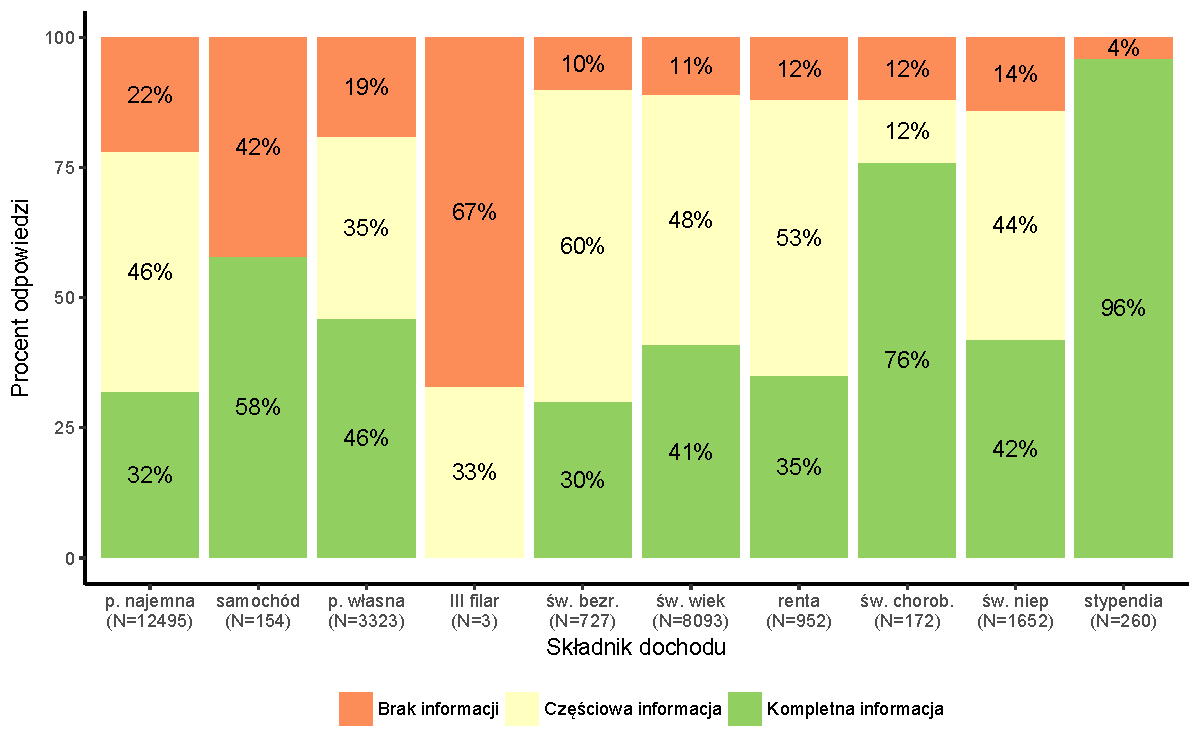
\includegraphics[width=0.8\textwidth]{04_wykresy/dochod_osoby_imputacja-1.pdf}
\caption{Odsetek imputowanych wartości dochodu w badaniu EU-SILC 2011 według kategorii dochodu}
\small{Źródło: opracowanie własne na podstawie badania EU-SILC 2011.}
\label{fig:dochod_osoby_imp}
\end{figure}

W większości przypadków odsetek braku informacji, a co za tym idzie całkowita imputacja wartości, nie przekraczał 22\% wszystkich odpowiedzi w ramach każdej z wyróżnionych kategorii. Wyjątkiem jest tu cecha: wykorzystanie samochodu służbowego do celów prywatnych brutto, gdzie brak informacji stanowił 42\%. Największy odsetkiem kompletnych danych charakteryzuje się cecha stypendia brutto --- 96\%.	

Następnie analizie poddano zależność pomiędzy sposobem odpowiedzi, a odsetkiem imputowanych wartości. Rysunek \ref{fig:dochod_osoby_imp_prox} przedstawia zestawienie struktury imputacji poszczególnych kategorii dochodu i struktury metody pozyskania odpowiedzi. Przy nazwach cech podano liczebności poszczególnych kategorii.

\begin{figure}[ht]
\centering
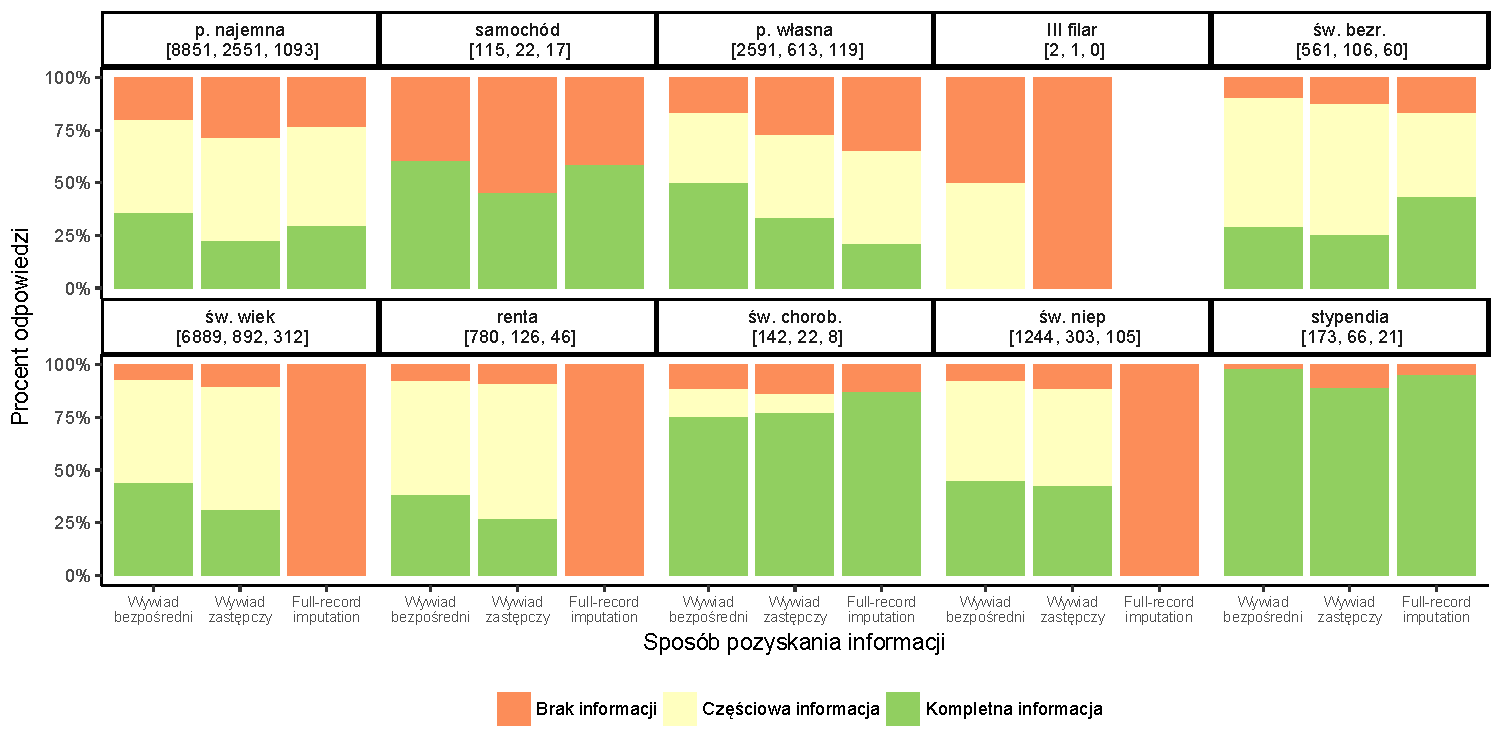
\includegraphics[width=0.8\textwidth]{04_wykresy/dochod_osoby_imputacja_proxy-1.pdf}
\caption{Odsetek imputowanych wartości dochodu w badaniu EU-SILC 2011 według kategorii dochodu oraz sposobu odpowiedzi}
\small{Źródło: opracowanie własne na podstawie badania EU-SILC 2011.}
\label{fig:dochod_osoby_imp_prox}
\end{figure}

We wszystkich kategoriach dochodu obserwowana jest większa frakcja wartości imputowanych w przypadku, gdy był przeprowadzany wywiad zastępczy. Mniejszy jest natomiast odsetek jednostek, dla których uzyskano kompletną informację o dochodzie. Należy jednak podkreślić to, że analizowane grupy były różnoliczne.

Rysunek \ref{fig:dochod_gosp} prezentuje dane dotyczące dochodów na poziomie gospodarstwa domowego. Także w tym przypadku z racji występowania obserwacji o bardzo dużych wartościach cechy w kategorii dochód z własności finansowej ograniczono oś Y do wartości 50 000 zł.

\begin{figure}[ht]
\centering
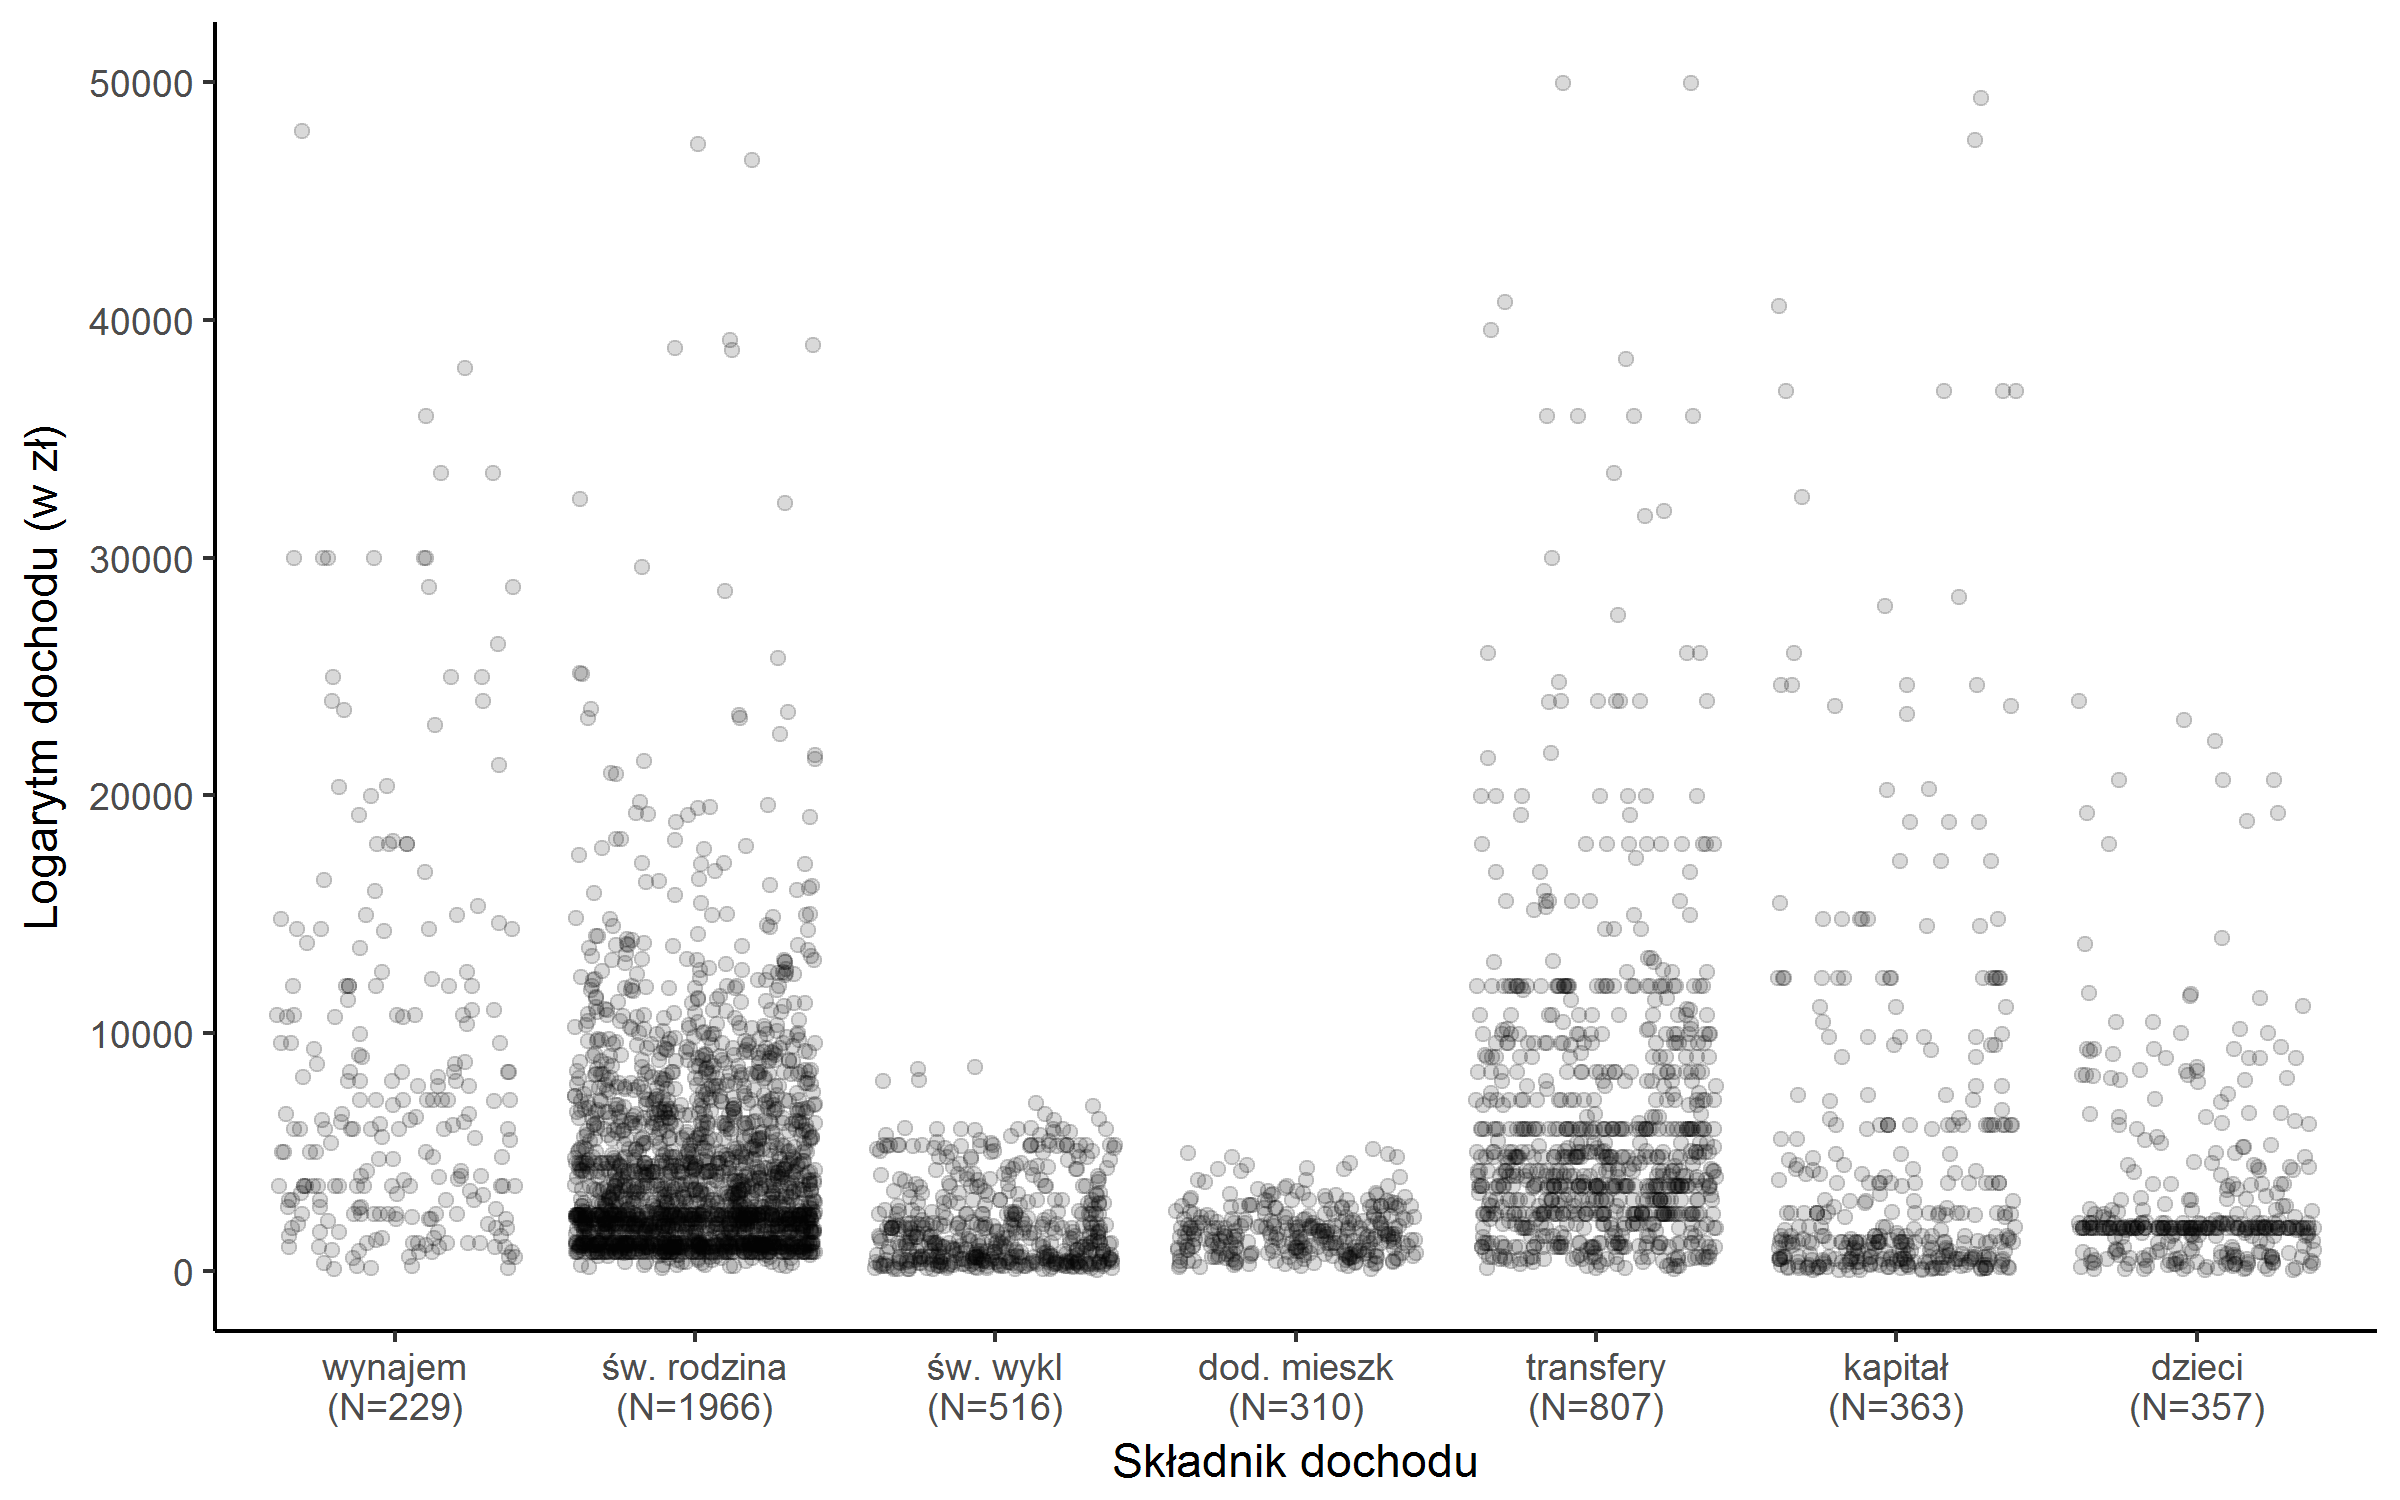
\includegraphics[width=0.8\textwidth]{04_wykresy/dochod_gospodarstw-1.png}
\caption{Wartości dochodu gospodarstw w badaniu EU-SILC 2011 według kategorii dochodu (do 50000 zł)}
\small{Źródło: opracowanie własne na podstawie badania EU-SILC 2011.}
\label{fig:dochod_gosp}
\end{figure}

W tym przypadku najczęściej występującą kategorią dochodu są świadczenia dotyczące rodziny (15,3\%) oraz regularne transfery pieniężne otrzymywane od osób spoza gospodarstwa domowego (6,3\%). Najrzadziej gospodarstwa deklarowały dochody pochodzące z wynajmu nieruchomości (1,8\%) oraz dodatków mieszkaniowych (2,4\%). Najwyższa wartość średnia występuje w kategorii dochód z własności finansowej (kapitałowy) brutto (15 443 zł). Ta sama kategoria cechuje się także wartością maksymalną (799 059 zł) oraz największym zróżnicowaniem (484,2\%).

W ramach najliczniejszej kategorii dochodu czyli świadczeń dotyczących rodziny występuje bardzo liczna grupa jednostek, dla których wartość cechy wynosi 815 zł. Także w przypadku dochodu dzieci do lat 16 obserwuje się liczne obserwacje, dla których cecha przyjmuje wartość równą 1 834 zł.

W ramach prowadzonej analizy wyznaczono także udział imputowanych wartości w poszczególnych kategoriach dochodu --- rysunek \ref{fig:dochod_gosp_imp}.

\begin{figure}[htp]
\centering
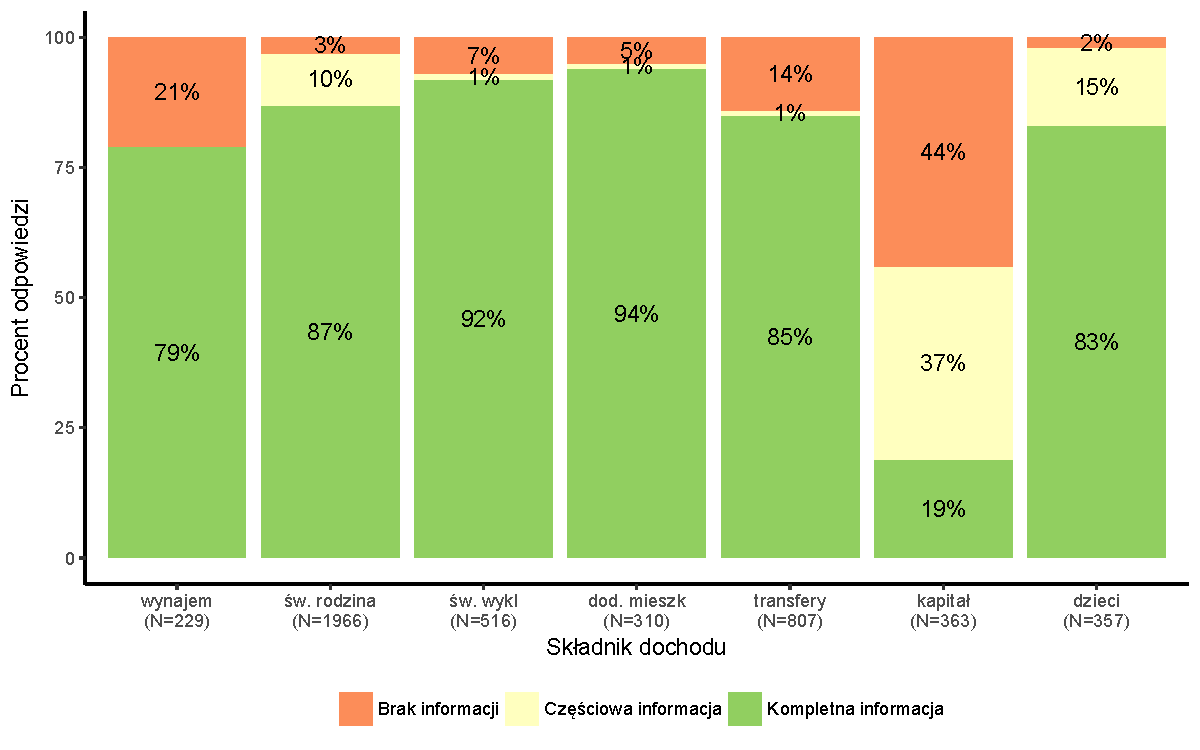
\includegraphics[width=0.8\textwidth]{04_wykresy/dochod_gospodarstw_imputacja-1.pdf}
\caption{Odsetek imputowanych wartości dochodu gospodarstw w badaniu EU-SILC 2011 według kategorii dochodu}
\small{Źródło: opracowanie własne na podstawie badania EU-SILC 2011.}
\label{fig:dochod_gosp_imp}
\end{figure}

W przypadku dochodu zbieranego na poziomie gospodarstwa większość informacji była kompletna. Wyjątkiem jest kategoria dochodu określająca dochód z własności finansowej (kapitałowej) brutto --- brak informacji stanowił tu 44\%, zaś częściową informację o dochodzie uzyskano w przypadku 37\% badanych jednostek.

Informacja na temat sposobu przeprowadzenia wywiadu jest przypisywana do konkretnej osoby w gospodarstwie, w związku z czym analiza zależności pomiędzy imputacją a przeprowadzeniem wywiadu na poziomie gospodarstwa nie była możliwa do przeprowadzenia.

Dalszą część analizy poświecono rozchodom. Na rysunku \ref{fig:trans_spol} przedstawiono rozkład transferów społecznych, które wpływają \emph{in minus} na dochód gospodarstwa domowego.

\begin{figure}[htp]
\centering
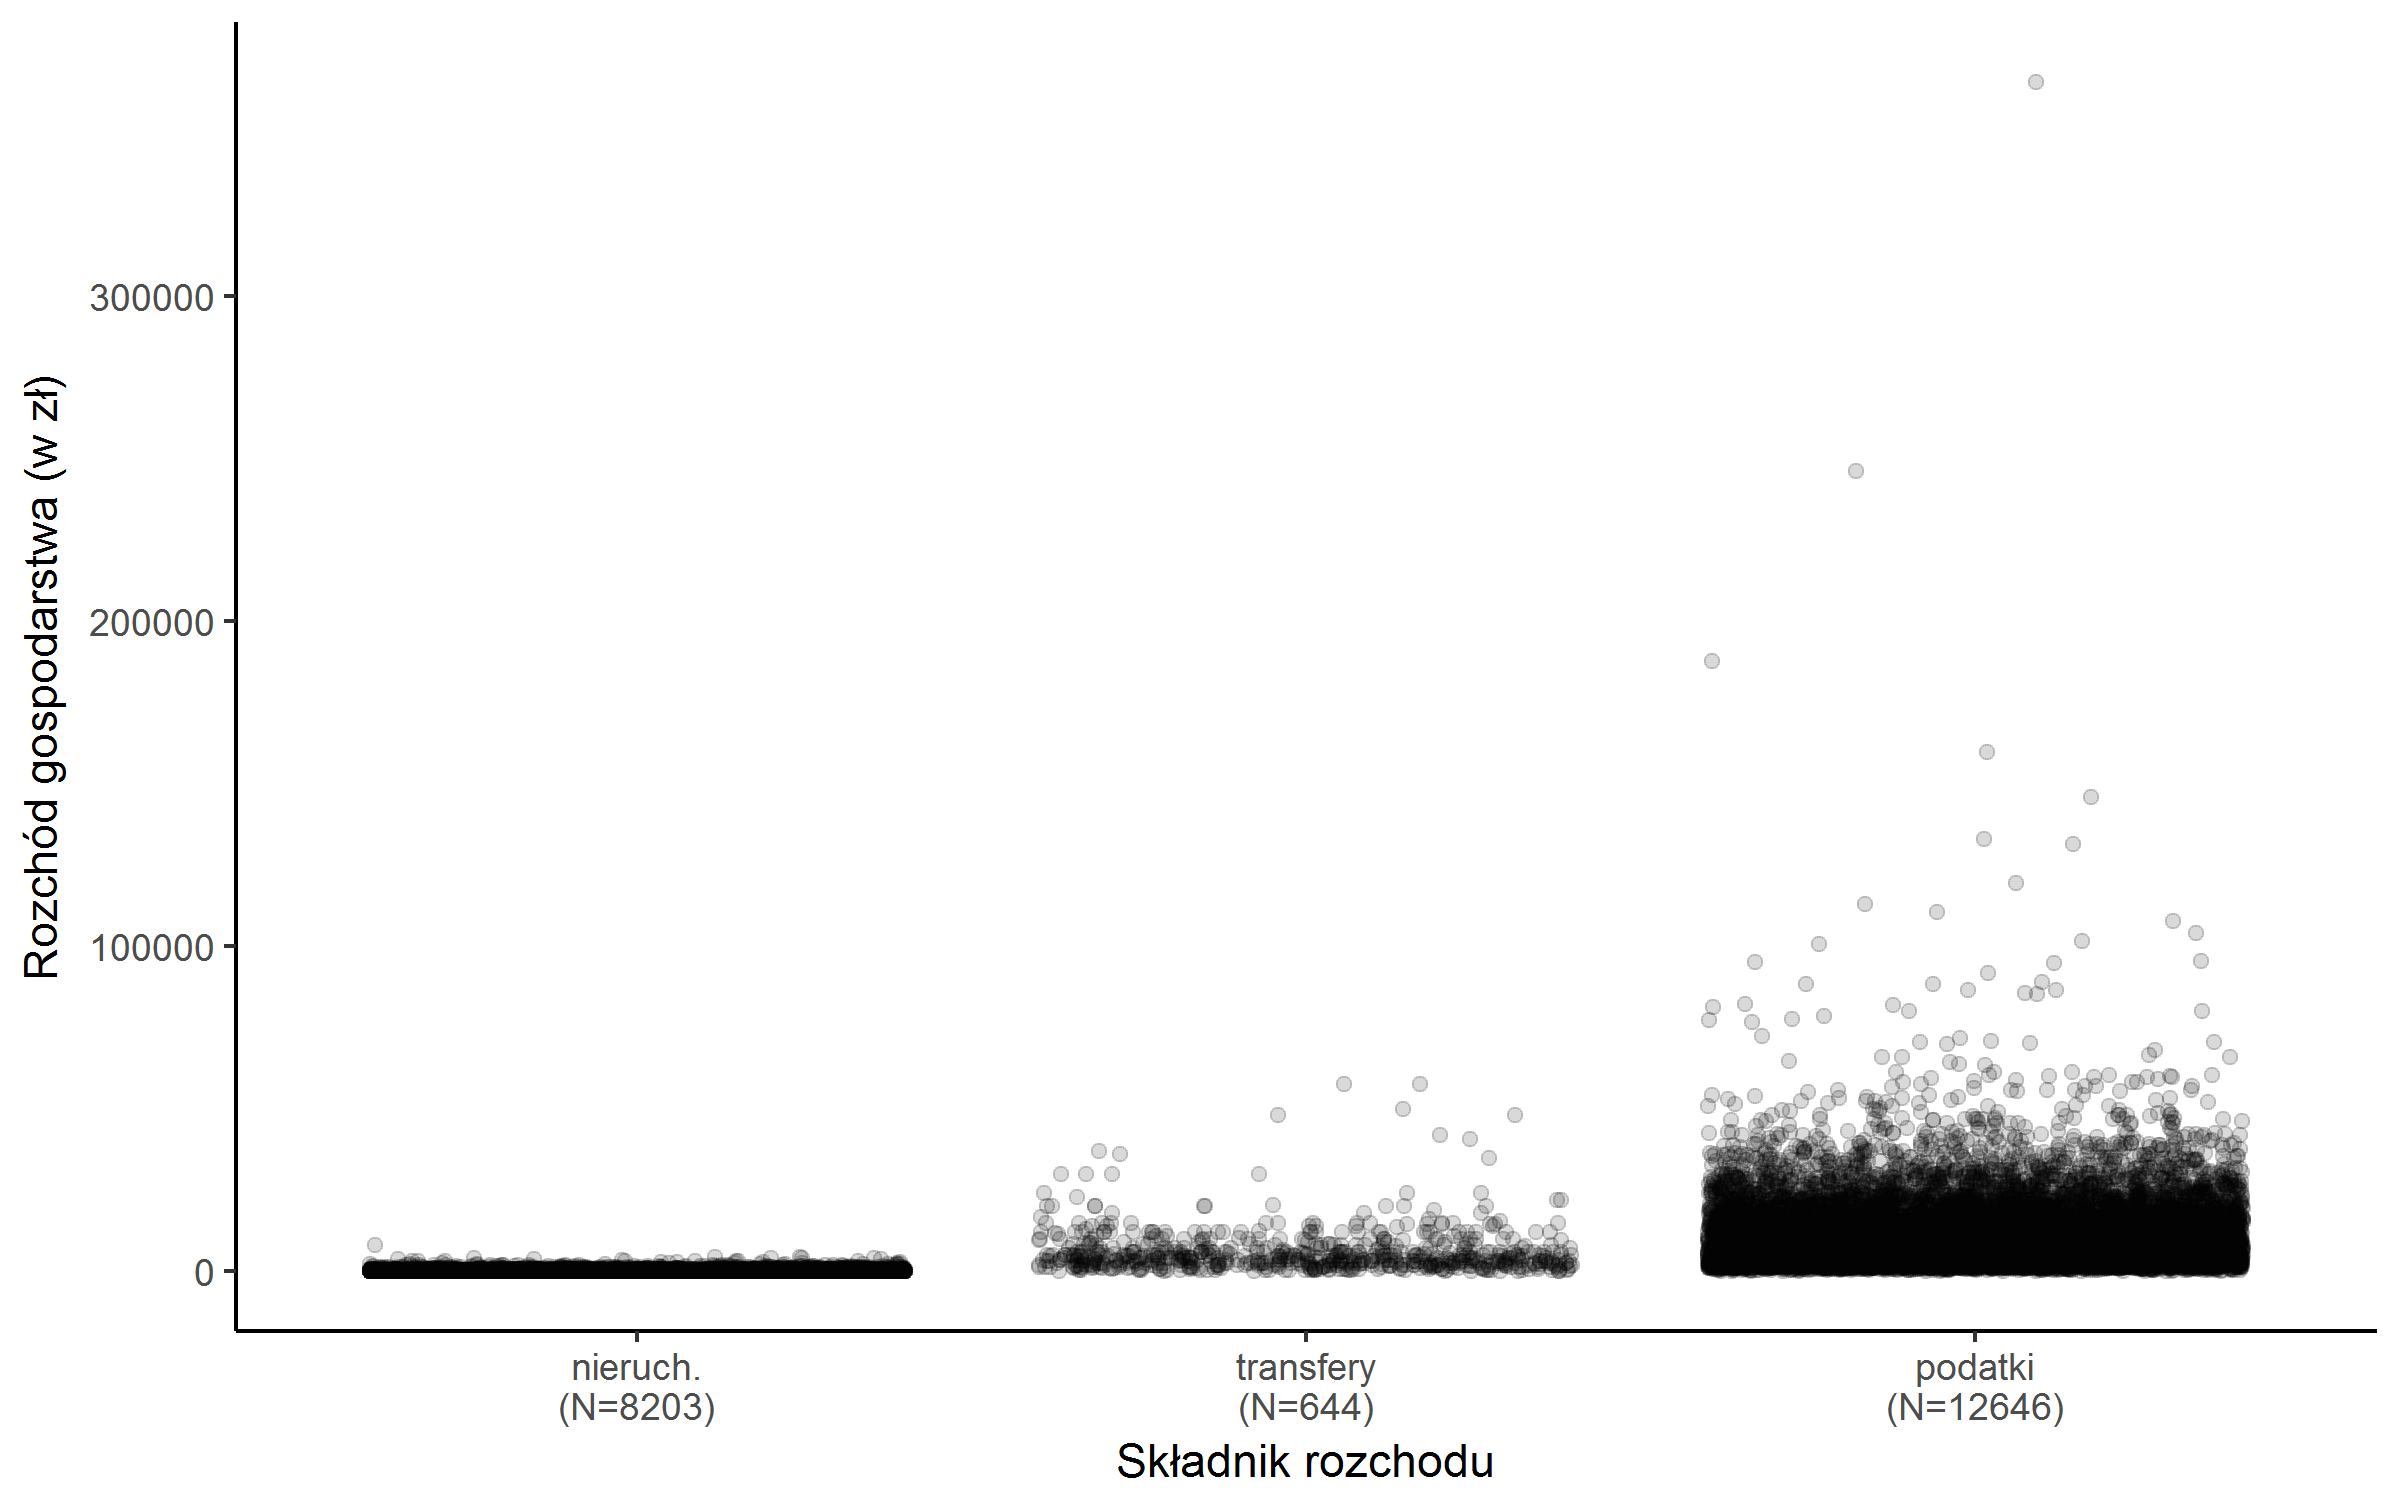
\includegraphics[width=0.8\textwidth]{04_wykresy/transfery_spoleczne-1.png}
\caption{Wartości transferów społecznych gospodarstw w badaniu EU-SILC 2011 według kategorii rozchodu}
\small{Źródło: opracowanie własne na podstawie badania EU-SILC 2011.}
\label{fig:trans_spol}
\end{figure}

Blisko 99\% badanych gospodarstw wykazało w swoich obciążeniach podatek dochodowy oraz składki na ubezpieczenie społeczne. Na drugim miejscu pod względem częstości znalazły się podatki od nieruchomości (63,7\%). Niewielki odsetek respondentów (5\%) wykazał regularne transfery pieniężne przekazywane osobom spoza gospodarstwa domowego. Najwyższa obserwowana wartość podatku odprowadzona przez gospodarstwo domowe wynosiła 365 822 zł.

W następnej kolejności wyznaczono frakcje poszczególnych sposobów imputacji (por. rysunek \ref{fig:trans_spol_imp}).

\begin{figure}[htp]
\centering
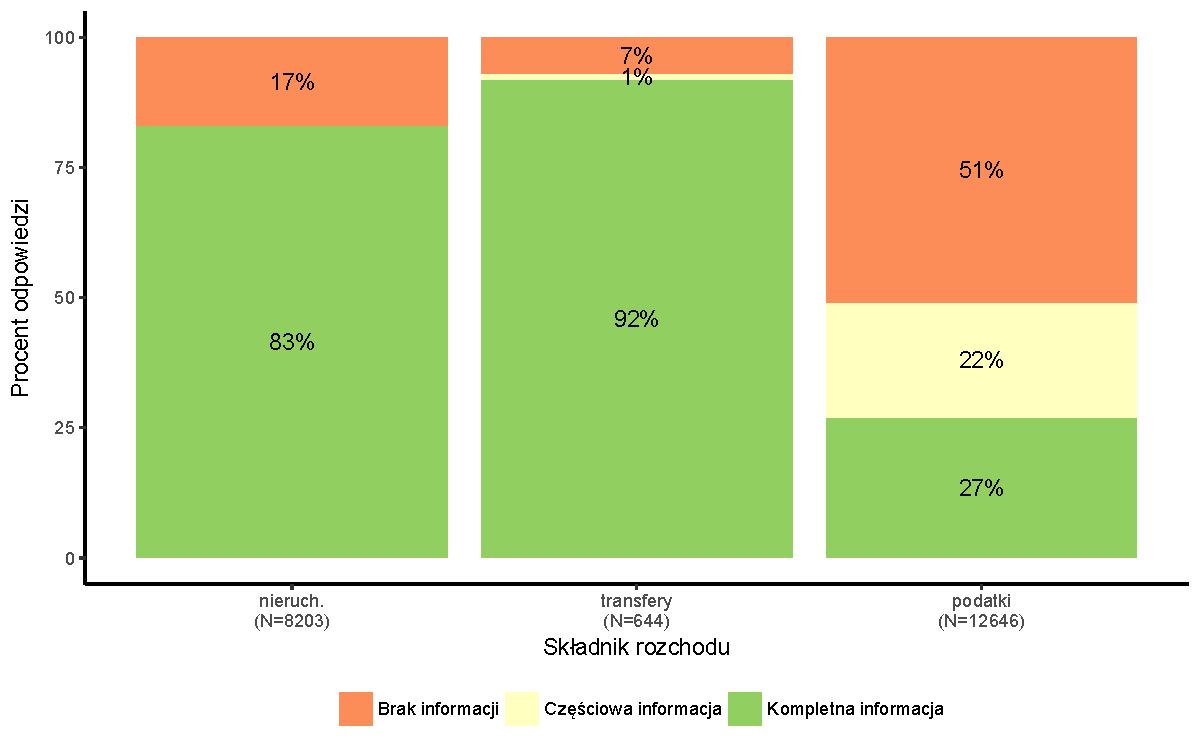
\includegraphics[width=0.8\textwidth]{04_wykresy/tranfery_spoleczne_imputacja-1.pdf}
\caption{Odsetek imputowanych wartości transferów społecznych w badaniu EU-SILC 2011 według kategorii rozchodu}
\small{Źródło: opracowanie własne na podstawie badania EU-SILC 2011.}
\label{fig:trans_spol_imp}
\end{figure}

W kategorii rozchodów największym zróżnicowaniem pod względem kompletności cechuje się podatek dochodowy, składki na ubezpieczenie społeczne brutto. Tylko 27\% respondentów przekazało na ten temat kompletną informację, natomiast dla 51\% jednostek wartość cechy musiała być całkowicie imputowana.

%\subsection{Dochód ekwiwalentny}

Na podstawie kategorii dochodów i rozchodów przedstawionych na początku niniejszego rozdziału, uzyskano wektor dochodów uwzględniający transfery społeczne. W analizach ekonomicznych dochód zwykle przelicza się uwzględniając wymiar demograficzny gospodarstwa domowego. Najprostszym tego typu przekształceniem jest obliczenie dochodu przypadającego na 1 osobę w~gospodarstwie. Takie podejście ma jednak wadę polegającą na nieuwzględnieniu zróżnicowania potrzeb osób w gospodarstwie wynikających z jego wielkości oraz wieku jego członków. Zastosowanie odpowiedniej skali ekwiwalentności umożliwia uwzględnienie tych różnic. Wykorzystując wzór na zmodyfikowaną skalę ekwiwalentności OECD i bazując na danych dotyczących liczby osób w wieku co najmniej 14 lat oraz poniżej tego wieku wyznaczono współczynniki ekwiwalentności. Na tej podstawie w analizowanym zbiorze danych zidentyfikowano 51 typów gospodarstw o różnych składach demograficznych. 

Najliczniej reprezentowaną grupą gospodarstw są gospodarstwa zamieszkiwane przez dwie osoby powyżej 14 roku życia. 73 procent wszystkich gospodarstw domowych stanowią gospodarstwa, w których nie występuje żadna osoba poniżej 14 roku życia. Ponadto w próbie znalazły się także gospodarstwa o bardzo dużej liczbie członków --- największe z nich składało się z 17 osób, w tym 4 osób poniżej 14 roku życia.

Uwzględniając skład demograficzny gospodarstwa wyznaczono wektor dochodów ekwiwalentnych, który stał się podstawą dalszych analiz. 

% Rozkład tego dochodu przedstawiony jest na rysunku \ref{fig:doch_ekw}.

% \begin{figure}[htp]
% 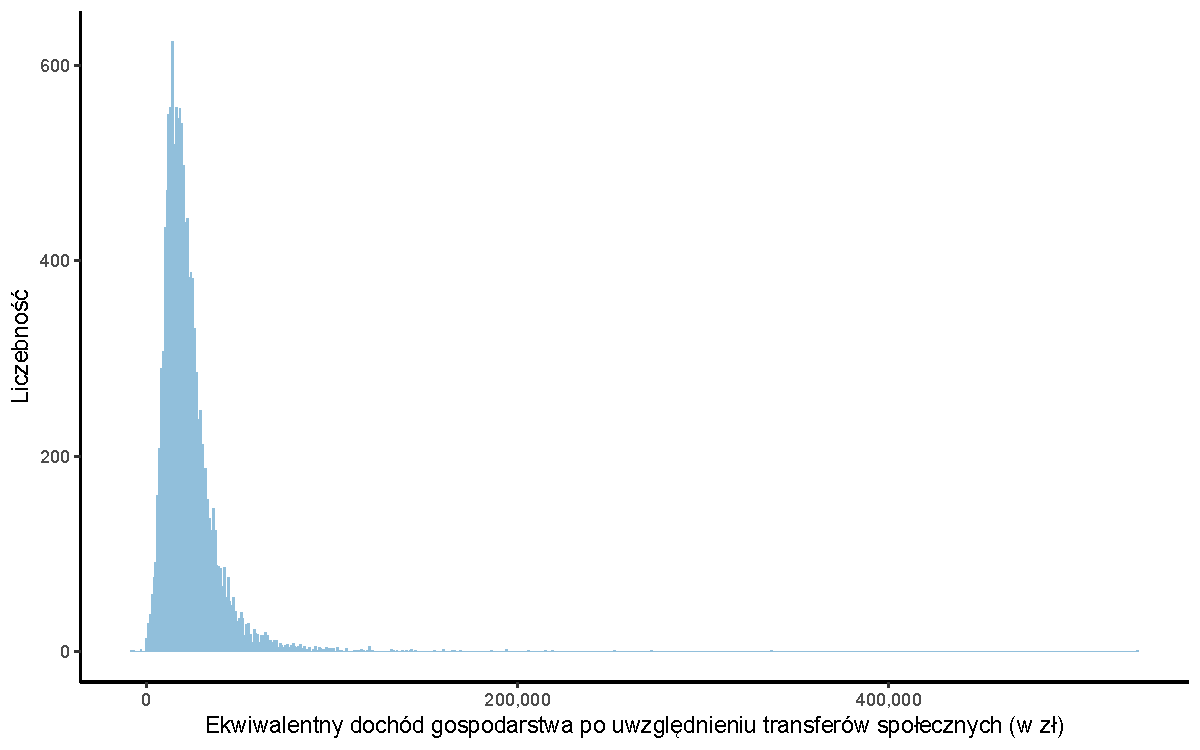
\includegraphics[width=\textwidth]{04_wykresy/dochod_ekiwalentny-1.pdf}
% \caption{Rozkład dochodu ekiwalentnego w badaniu EU-SILC 2011}
% \small{Źródło: opracowanie własne na podstawie badania EU-SILC 2011.}
% \label{fig:doch_ekw}
% \end{figure}

Średni dochód ekwiwalentny wyniósł 22 453 zł, natomiast mediana 19 130 zł. Rozkład dochodów gospodarstw domowych charakteryzował się bardzo dużym zróżnicowaniem --- współczynnik zmienności wynosił 71\%. Znaną powszechnie własnością rozkładu dochodu jest jego silna asymetria prawostronna --- w tym przypadku trzeci moment centralny był równy 6,23. W badaniu EU-SILC 2011 znalazło się 14 gospodarstw, których dochody były ujemne. Minimalna wartość dochodu wynosiła -7 800 zł. Z kolei w siedmiu gospodarstwach domowych dochód ekwiwalentny przekraczał 200 tys. złotych. Gospodarstwa te znajdowały się w powiatach: krapkowickim (województwo opolskie), m. Gdańsk, złotoryjski (dolnośląskie), m. st. Warszawa, m. Lublin (lubelskie). Maksymalna wartość rocznego dochodu ekwiwalentnego wynosiła 534 337 zł (powiat krapkowicki).

\section{Analiza próby}

Pierwszym etapem w estymacji dla małych domen jest analiza liczebności próby oraz określenie liczby reprezentantów posiadających badaną cechę (fakt przynależności do sfery ubóstwa).

\subsection{Liczebność próby i reprezentantów}

Z punktu widzenia estymacji dla małych obszarów bardzo ważne zagadnienie stanowi liczebność całej próby oraz liczba jednostek --- reprezentantów posiadających określony wariant badanej cechy. W przypadku analizy ubóstwa tą cechą będzie przynależność do sfery niedostatku. Dana domena może być licznie reprezentowana w próbie, a mimo to estymacja będzie niemożliwa z~powodu braku ubogich jednostek. W niniejszej analizie za granicę ubóstwa przyjęto 60\% mediany dochodów ekwiwalentnych, która w 2011 roku wynosiła 12 045 zł (por. podrozdział \ref{pr:identyfikacja-ubostwa}).

Na rysunku \ref{fig:proba_reprez} zestawiono liczebność próby oraz reprezentantów w nieplanowanych domenach tj. podregionach i powiatach.

\begin{figure}[htp]
\centering
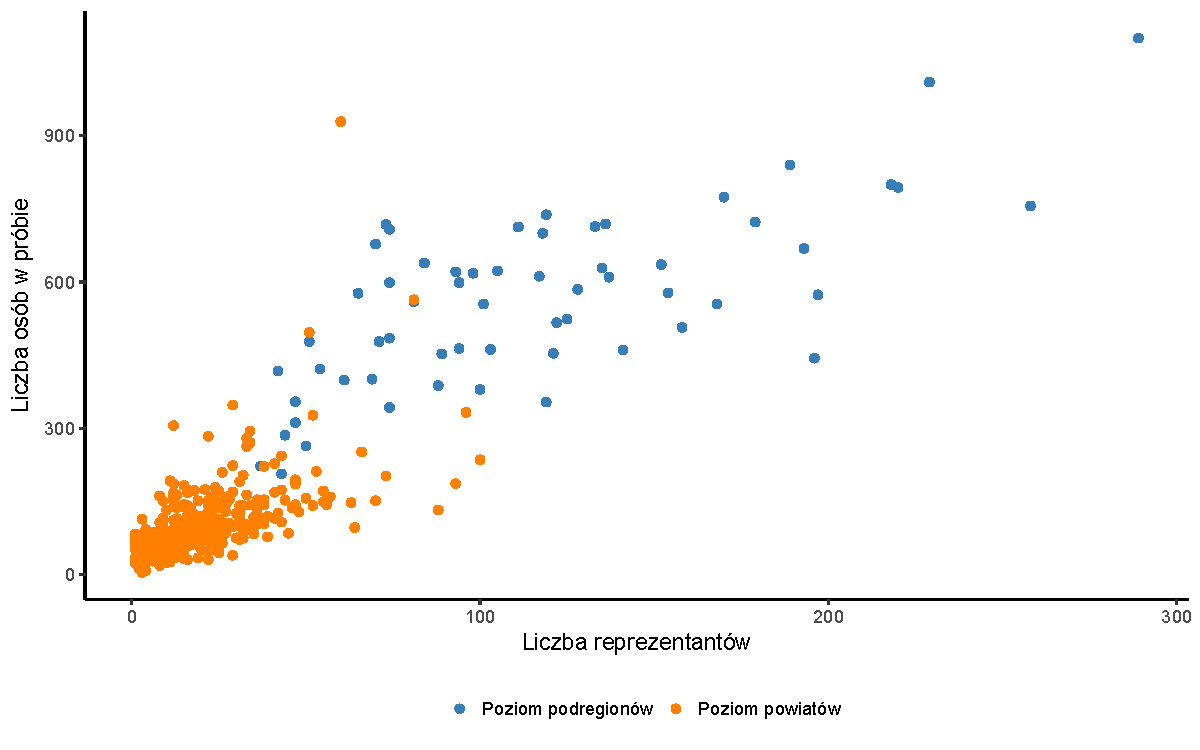
\includegraphics[width=0.8\textwidth]{04_wykresy/liczebnosc_proby_i_reprezentantow-1.pdf}
\caption{Liczba osób w próbie oraz liczba osób ubogich w badaniu EU-SILC 2011 w~przekroju podregionów i powiatów}
\small{Źródło: opracowanie własne na podstawie badania EU-SILC 2011.}
\label{fig:proba_reprez}
\end{figure}

Spośród podregionów najmniej licznie były reprezentowane podregiony ełcki (207 osób w~gospodarstwach domowych), stargardzki (223) oraz suwalski (264). Z kolei największą liczbę reprezentantów odnotowano w podregionach kieleckim (1 100), ostrołęcko-siedleckim (1 010) oraz Warszawie (929).

Rozkład próby w powiatach, których liczba jest prawie 6-krotnie większa niż liczba podregionów był odmienny. Cztery powiaty w ogóle nie były reprezentowane w zrealizowanej próbie --- powiat wieruszowski, proszowicki, moniecki oraz włoszczowski. Minimalna liczba osób w reprezentowanym powiecie wynosiła 4 --- powiat rypiński oraz skierniewicki, z kolei najwięcej osób zbadano w Warszawie (929) oraz innych miastach na prawach powiatu takich jak Łódź (564) czy Kraków (497). Sześć podregionów jest równocześnie miastami na prawach powiatu: Łódź, Warszawa, Kraków, Poznań, Szczecin i Wrocław. Zdarzają się także powiaty, przede wszystkim miasta na prawach powiatu, w których liczba osób w próbie była wyższa niż w niektórych podregionach. Przykładowo, w powiecie kieleckim w próbie znalazło się więcej osób aniżeli w całym podregionie łódzkim składającym się z trzech powiatów.

Najmniej reprezentantów osób ubogich odnotowano w Poznaniu (22), na kolejnym miejscu jest Wrocław (29) oraz Szczecin (34). Z kolei najliczniej osoby ubogie występowały w podregionach kieleckim (289), chełmsko-zamojskim (258) oraz ostrołęcko-siedleckim (229).

Analiza prowadzona na poziomie powiatów pokazuje, że w 12 powiatach nie znalazła się ani jedna osoba uboga, co uniemożliwia estymację bezpośrednią dla tych jednostek. Natomiast w~7~powiatach znalazł się tylko 1 reprezentant zbiorowości osób żyjących w niedostatku. Najwięcej osób ubogich zidentyfikowano w powiecie lubelskim (100), na kolejnym miejscu znalazł się powiat kielecki (96), a za nim powiat tarnowski (93).

Pomiędzy liczbą osób w próbie a liczbą reprezentantów występuje silna dodatnia zależność. Współczynnik korelacji rang Spearmana na poziomie podregionów wynosi 0,64, natomiast na poziomie powiatów 0,68.

W przypadku estymacji wskaźnika określającego głębokość ubóstwa wykorzystywane są te same jednostki, co dla stopy ubóstwa, w związku z czym liczebność reprezentantów będzie taka sama.

\subsection{Jakość oszacowań bezpośrednich wskaźników ubóstwa}

Na podstawie liczby zidentyfikowanych osób ubogich z wykorzystaniem estymatora Horvitza-Thompsona oraz wag przekrojowych z badania EU-SILC oszacowano stopę oraz głębokość ubóstwa na poziomie podregionów i powiatów. W pierwszej kolejności przeanalizowano zmienność otrzymanych oszacowań (por. rys. \ref{fig:zmiennosc_ht}).

\begin{figure}[htp]
\centering
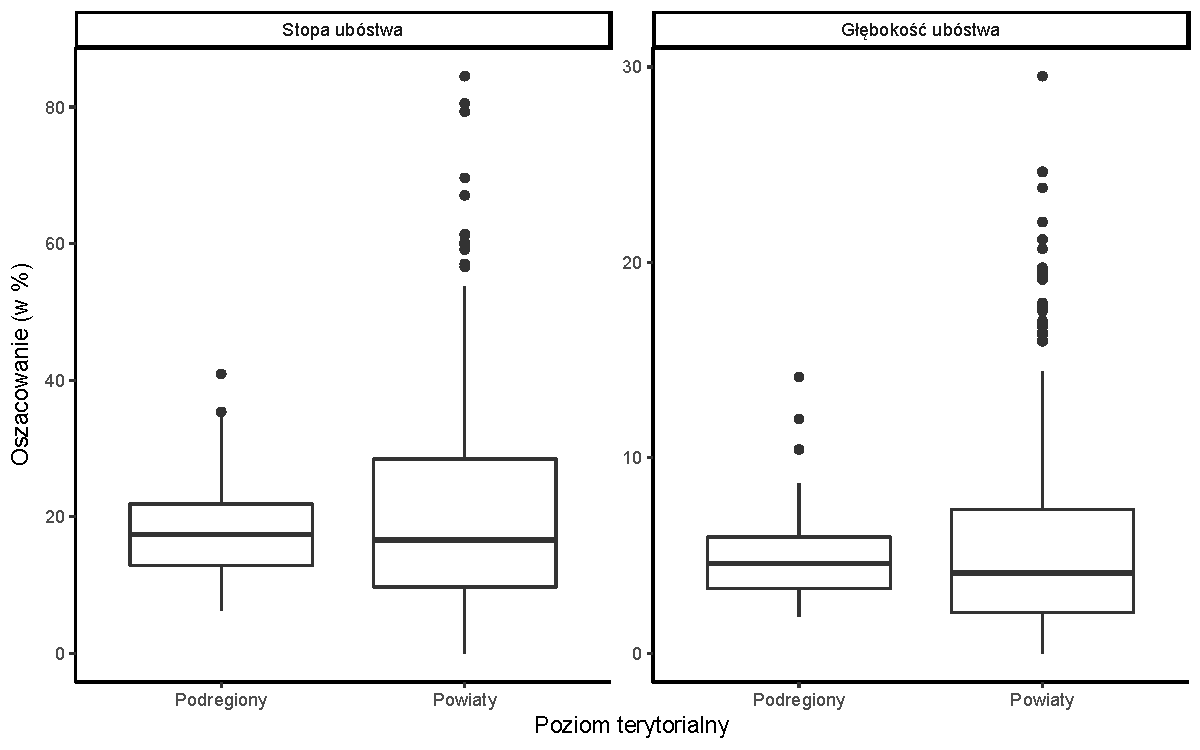
\includegraphics[width=0.8\textwidth]{04_wykresy/zmiennosc_ht-1.pdf}
\caption{Rozkład oszacowań bezpośrednich stopy oraz głębokości ubóstwa w przekroju podregionów i powiatów}
\small{Źródło: opracowanie własne na podstawie badania EU-SILC 2011.}
\label{fig:zmiennosc_ht}
\end{figure}

Wartości przeciętne w ramach każdego z badanych wskaźników w analizowanych przekrojach terytorialnych są zbliżone. Średnia wartość stopy ubóstwa w podregionach wynosi 18\%, natomiast na poziomie powiatów 20\%. Mediana w obu przypadkach jest taka sama --- 17\%. Z kolei średni poziom głębokości ubóstwa wynosi 5\% zarówno na poziomie powiatów i podregionów. Główna różnica w rozkładzie wskaźników wynika ze zróżnicowania. Oszacowania stopy ubóstwa na poziomie podregionów charakteryzują się wartością współczynnika zmienności równą 42\%, a dla głębokości ubóstwa 48\%. Z kolei na poziomie powiatów te wartości są prawie dwukrotnie wyższe --- 74\% dla oszacowań stopy ubóstwa i 89\% dla oszacowań głębokości ubóstwa. Na poziomie powiatów obserwuje się bardzo małe i duże wartości oszacowań wskaźników ubóstwa --- z jednej strony bliskie zeru, a z drugiej przekraczające 80\%. Występowanie takich wartości stopy czy głębokości ubóstwa w rzeczywistości jest wysoce nieprawdopodobne, co wskazuje na niedoskonałość oszacowań bezpośrednich w sytuacji nielicznej próby.

Kryterium oceny jakości estymowanych wskaźników był względny błąd szacunku będący ilorazem błędu standardowego oszacowania i oceny estymatora (ang. \textit{Relative Root Mean Square Error} --- RRMSE). W publikacjach GUS określany jest on jako wskaźnik precyzji. Istnieją dwa podejścia do estymacji błędu oszacowania. Pierwsze z nich zakłada zastosowanie estymatorów odpowiednich dla prostego schematu losowania. Podejście to wynika z przyjęcia założenia, że małe domeny, dla których dokonywana jest analiza nie były uwzględnione na etapie projektowania badania, a zatem nie należy dla nich wykorzystywać informacji na temat schematu losowania. Z kolei drugie podejście wskazuje, że należy te informacje wykorzystać także przy szacowaniu wariancji dla nieplanowanych domen. Niezależnie jednak od rodzaju prowadzonego badania wykorzystanie złożonego schematu losowania powoduje, że otrzymane błędy oszacowań są wyższe \citep{lehtonen2004}. Jest to szczególnie widoczne w przypadku domen, w których próba jest bardzo nieliczna.

W badaniu EU-SILC są dostępne informacje dotyczące jednostek losowania pierwszego stopnia oraz warstw losowania. Wobec tego możliwa jest estymacja wariancji oszacowań wskaźników ubóstwa z wykorzystaniem zaimplementowanego w badaniu złożonego schematu losowania i metody bootstrap. Otrzymane w ten sposób wyniki zestawiono z oszacowaniami uzyskanymi przy założeniu prostego schematu losowania. W metodzie bootstrap losowano 500 podpróbek.

W ramach oceny jakości wyników otrzymanych na podstawie estymacji bezpośredniej w pierwszej kolejności porównano względne błędy oszacowań oraz liczbę reprezentantów --- osób ubogich w przekroju podregionów. Wyniki przedstawiono na rysunku \ref{fig:prec_ht_podreg}.

\begin{figure}[htp]
\centering
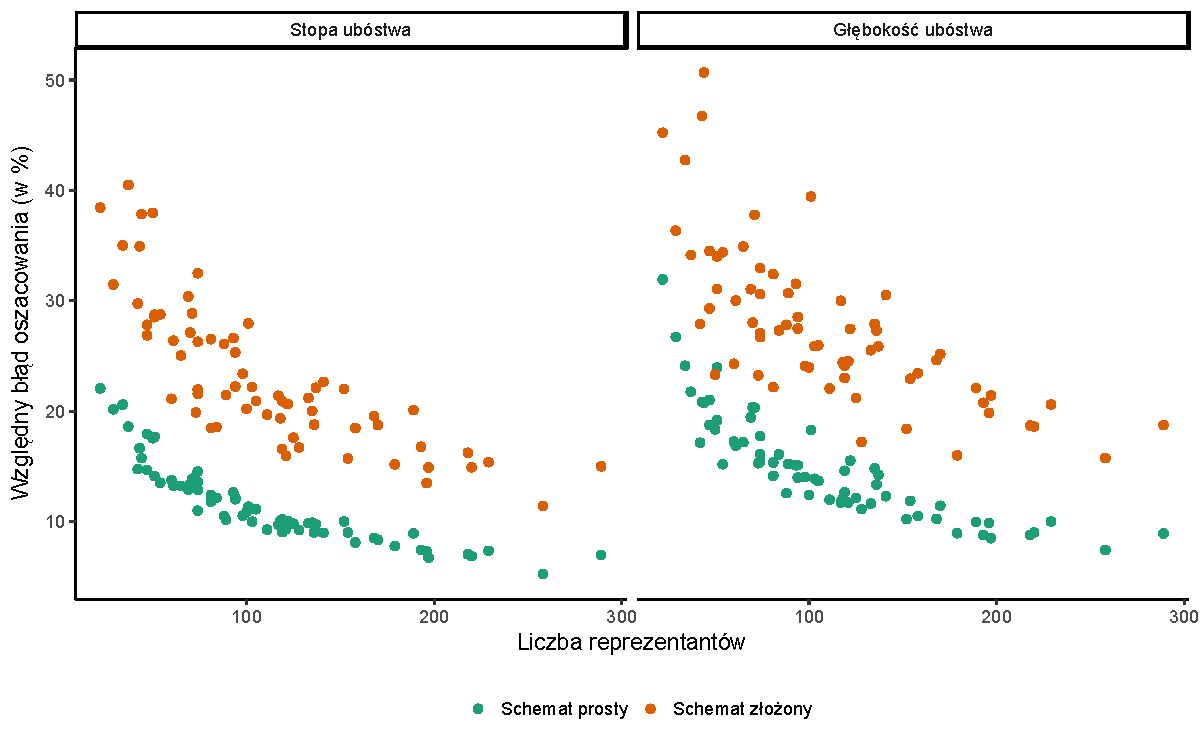
\includegraphics[width=0.8\textwidth]{04_wykresy/precyzja_ht_podreg-1.pdf}
\caption{Porównanie względnych błędów oszacowań i liczby reprezentantów dla stopy oraz głębokości ubóstwa w przekroju podregionów}
\small{Źródło: opracowanie własne na podstawie badania EU-SILC 2011.}
\label{fig:prec_ht_podreg}
\end{figure}

Średnia wartość względnego błędu oszacowania stopy ubóstwa wynosiła 12\% dla schematu prostego i 23\% dla schematu złożonego. W przypadku głębokości ubóstwa przeciętny względny błąd kształtował się na poziomie odpowiednio 15\% i 28\%. Otrzymane wielkości wskazują na to, że wykorzystanie złożonego schematu losowania dwukrotnie zwiększa wartość względnych błędów standardowych w porównaniu do schematu zakładającego losowanie proste. W przypadku stopy ubóstwa dla schematu prostego minimalna wartość wskaźnika precyzji wynosiła 5,2\%, natomiast dla schematu złożonego 11,4\% --- podregion chełmsko-zamojski. Najwyższe względne błędy oszacowań otrzymano dla podregionu m. Poznań (22\%) przy założeniu schematu prostego oraz dla podregionu starogardzkiego (40,5\%) w przypadku schematu złożonego. Wskaźnik głębokości ubóstwa charakteryzuje się wyższymi wartościami względnych błędów oszacowań. Minimum wynoszące 7,4\% dla schematu prostego oraz 15,7\% dla schematu złożonego zanotowano dla podregionu chełmsko-zamojskiego. Najwyższa wartość względnego błędu dla głębokości ubóstwa wynosiła 31,9\% dla podregionu m. Poznań (schemat prosty) oraz 50,7\% dla podregionu szczecińskiego (schemat złożony). Na rysunku można także zaobserwować silną zależność pomiędzy wskaźnikiem precyzji, a liczbą reprezentantów osób ubogich. Współczynnik korelacji rang Spearmana dla wskaźnika stopy ubóstwa wyniósł $r_S=-0,97$ przy założeniu schematu prostego oraz $r_S=-0,86$ przy założeniu schematu złożonego. W przypadku głębokości ubóstwa miary korelacji są następujące: $r_S=-0,92$ dla schematu prostego oraz $r_S=-0,76$ dla schematu złożonego.

Porównano także względne błędy oszacowań na poziomie powiatów. W celu zapewnienia czytelności rysunku \ref{fig:prec_ht_pow} oś OY została ograniczona do wartości 200\%.

\begin{figure}[htp]
\centering
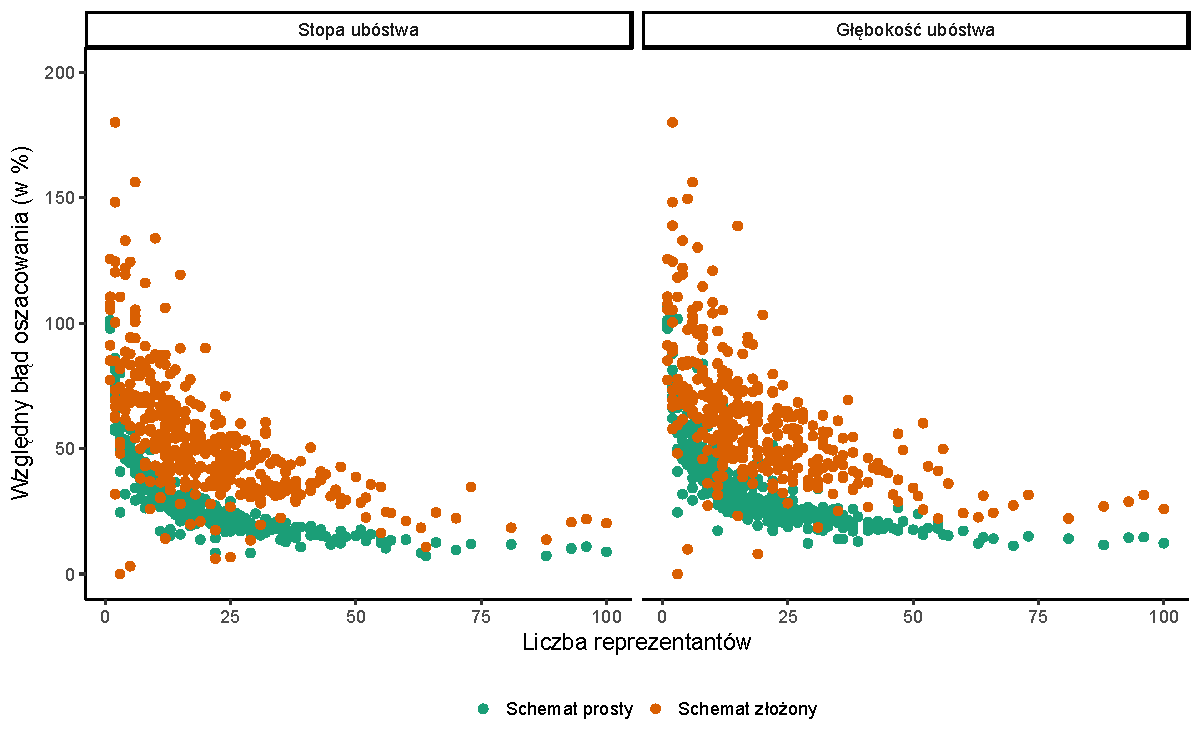
\includegraphics[width=0.8\textwidth]{04_wykresy/precyzja_ht_pow-1.pdf}
\caption{Porównanie względnych błędów oszacowań i liczby reprezentantów dla stopy oraz głębokości ubóstwa w przekroju powiatów}
\small{Źródło: opracowanie własne na podstawie badania EU-SILC 2011.}
\label{fig:prec_ht_pow}
\end{figure}

W przypadku powiatów wykorzystanie złożonego schematu losowania także spowodowało dwukrotny wzrost przeciętnej wartości wskaźnika precyzji. Średni poziom wskaźnika precyzji stopy ubóstwa wyniósł 31\% dla schematu prostego i 59\% dla schematu złożonego. Głębokość ubóstwa cechowały przeciętne wartości błędów równe odpowiednio 36\% i 66\%. O ile maksymalna wartość wskaźnika w przypadku zastosowania prostego schematu losowania wynosiła 107\%, o tyle przy schemacie złożonym było to 749\% (powiat myśliborski w województwie zachodniopomorskim). Ponadto na rysunku nie znalazły się oszacowania błędów wskaźników ubóstwa dla powiatu kolneńskiego (369\%), milickiego (347\%), brzozowskiego (322\%) oraz nidzickiego (246\%). Podobnie jak na poziomie podregionów obserwowana była zależność pomiędzy względnym błędem oszacowania a liczbą reprezentantów. Współczynnik korelacji rang Spearmana wyniósł $r_S=-0,93$ dla stopy ubóstwa w przypadku zastosowania schematu prostego oraz $r_S=-0,72$ w przypadku schematu złożonego. Dla głębokości ubóstwa były to odpowiednio wartości $r_S=-0,90$ i $r_S=-0,70$.

Z teorii metody reprezentacyjnej wiadomo, że estymator bezpośredni jest bardziej efektywny w przypadku zastosowania prostego schematu losowania \citep{bracha1996}. Ponadto wartość błędu oszacowania zależy od liczby jednostek wykorzystanych do estymacji wskaźnika. Ta zależność jest słabsza w przypadku zastosowania złożonego schematu losowania. W związku z tym, w dalszych obliczeniach przyjęto względny błąd wskaźników ubóstwa oszacowany z wykorzystaniem schematu prostego.

\section{Estymacja pośrednia wskaźników ubóstwa}

Kolejnym etapem badania było oszacowanie wskaźników ubóstwa na poziomie podregionów i~powiatów. Z uwagi na wysokie błędy standardowe oszacowań bezpośrednich wskaźników ubóstwa, a tym samym ich niską precyzję, podjęto próbę zastosowania estymacji pośredniej zamiast klasycznego podejścia. Estymacja charakterystyk ubóstwa z wykorzystaniem metod statystyki małych obszarów wymaga użycia tzw. \textit{zmiennych pomocniczych}. Celem zastosowania tych cech jest poprawa jakości estymacji, w związku z czym powinny one pochodzić ze źródeł pozbawionych błędów losowych --- np. z badań pełnych bądź rejestrów administracyjnych. W przypadku stosowania podejścia modelowego kluczowy jest dobór odpowiednich zmiennych, które dobrze opisują zróżnicowanie estymowanych cech. Nieodpowiednia specyfikacja zmiennych niezależnych może powodować obciążenie wyników.

W zależności od wykorzystywanego typu modelu, obszarowego czy jednostkowego, zmienne pomocnicze przyjmują inną postać. W pierwszym przypadku rolę zmiennych niezależnych pełnią zwykle wskaźniki społeczno-demograficzne wyliczone na poziomie danego obszaru --- podregionu bądź powiatu. Głównym źródłem takich cech są ogólnodostępne bazy danych statystycznych np. Bank Danych Lokalnych. Na potrzeby pracy utworzono bazę zmiennych pomocniczych zawierającą 1151 cech ekonomicznych, społecznych oraz demograficznych. Z kolei w podejściu jednostkowym wykorzystuje się informacje dostępne na poziomie pojedynczego gospodarstwa domowego. W tym przypadku konieczny jest dostęp do danych jednostkowych z badania pełnego lub rejestru administracyjnego. Główną przeszkodą w tworzeniu modelu wskaźników ubóstwa jest odróżnienie przyczyn od skutków niedostatku. Przykładowo, osoby ubogie mają zazwyczaj niższe wykształcenie, jednak nie można określić czy niskie wykształcenie zostało spowodowane przez niedostatek czy też bieda panująca w gospodarstwie domowym nie pozwoliła na zdobycie wyższego wykształcenia.

Do obliczeń wykorzystano środowisko R \citep{r2016} w obrębie którego zastosowano funkcje \emph{eblupFH} oraz \emph{eblupSFH} pochodzące z pakietu \emph{sae} \citep{molina-marhuenda2015} w celu oszacowania wskaźników ubóstwa z wykorzystaniem podejścia obszarowego. Do oceny błędu standardowego oraz obciążenia otrzymanych wskaźników zaimplementowano metodę bootstrap z~liczbą replikacji równą 500. Z kolei w aplikacji podejścia jednostkowego korzystano z funkcji \emph{lmer} zaimplementowanej w pakiecie \emph{lme4} \citep{lme42015}, własnych programów oraz funkcji wypracowanych w ramach projektu SAMPLE. Kody wypracowane w programie R zostały zamieszczone w~załączniku.

\subsection{Poziom podregionów}

Rok 2011 był ostatnim rokiem, w którym GUS opublikował dane dotyczące stopy ubóstwa na poziomie województw. Zwiększenie zakresu dostępnych informacji wymaga uwzględnienia niższego poziomu agregacji przestrzennej --- w tym przypadku będzie to poziom podregionów. W latach 2008--2014 w Polsce obowiązywał podział na 66 podregionów. Zmiana nastąpiła w 2015 roku, kiedy to rozdzielono większe podregiony i w ten sposób uzyskano 72 podregionów.

\subsubsection{Modelowanie stopy oraz głębokości ubóstwa na poziomie podregionów}\label{pr:model-podreg}

Punktem wyjścia w pracach nad estymacją wskaźników ubóstwa był model wypracowany w ramach współpracy Głównego Urzędu Statystycznego z Bankiem Światowym \citep{mapowanie2014,wawrowski2014}. Opracowany wówczas model wykorzystywał najprostsze rozwiązania, ponieważ był dedykowany statystyce publicznej. W niniejszej rozprawie zostanie podjęta próba poprawy tego modelu poprzez weryfikację zawartych w nim zmiennych pomocniczych oraz zastosowanie transformacji zmiennej zależnej w celu poprawy własności rozkładu cechy zależnej.

Model będący przedmiotem dyskusji miał na celu estymację wyłącznie stopy ubóstwa i zawierał następujące zmienne niezależne:

\begin{itemize}
\item odsetek osób samotnych powyżej 25 roku życia,
\item liczba pokoi przypadająca na członka gospodarstwa domowego,
\item odsetek gospodarstw domowych posiadających łazienkę,
\item odsetek gospodarstw domowych z dwiema osobami powyżej 25 roku życia z wykształceniem co najwyżej zawodowym,
\item gęstość zaludnienia,
\item stosunek liczby osób wymeldowanych do liczby zameldowanych na pobyt stały w podregionie.
\end{itemize}

W powyższym modelu dwie zmienne niezależne były nieistotne: gęstość zaludnienia oraz stosunek liczby osób wymeldowanych do liczby zameldowanych na pobyt stały w podregionie. Pozostawiono je jednak w modelu ze względów merytorycznych.

W tej części pracy podjęto próbę wypracowania nowego modelu zawierającego wyłącznie istotne zmienne niezależne. Przeanalizowano także możliwości przekształcenia zmiennej zależnej oraz rozszerzono zakres estymacji o wskaźnik głębokości ubóstwa. 

Biorąc pod uwagę dorobek polskich badaczy, jak i publikacje GUS przeanalizowano możliwe determinanty ubóstwa w kontekście ich wykorzystania w modelu ubóstwa. Ze względu na ograniczony dostęp do danych znalezienie ilościowych odpowiedników nie zawsze było możliwe dla wszystkich ustalonych symptomów.

Na podstawie potencjalnych determinant ustalonych w podrozdziale \ref{pr:determinanty} oraz danych dostępnych w Banku Danych Lokalnych dokonano wyboru szeregu wskaźników stanowiących potencjalne zmienne niezależne (pomocnicze) w modelu, w którym zmienną zależną był wskaźnik ubóstwa --- stopa oraz głębokość ubóstwa. Wśród rozpatrywanych zmiennych niezależnych znalazły się m.in. wskaźniki zależności demograficznej, odsetek osób mieszkających na wsi, wskaźniki aktywności ekonomicznej. Analizowano także dane dotyczące rodzin i na ich postawie utworzono wskaźniki określające udział rodzin z dziećmi pozostającymi na utrzymaniu w ogólnej liczbie rodzin w~Polsce z różną liczbą dzieci.

Zmienne opisujące zmienność stopy oraz głębokości ubóstwa zostały wybrane z wykorzystaniem metody krokowej wprzód. W tym celu wykorzystano funkcję \emph{selection} z pakietu FWDselect \citep{fwdselect2015}. Wybrany model był następnie merytorycznie weryfikowany. Badano poprawność znaku stojącego przy parametrze regresji pod kątem wpływu danej zmiennej na poziom ubóstwa oraz statystyczną istotność tego parametru.

W modelu objaśniającym stopę ubóstwa znalazły się następujące zmienne: udział rodzin z~3~dzieci poniżej 24 roku życia pozostających na utrzymaniu w liczbie rodzin z dziećmi poniżej 24 roku życia, odsetek mieszkań posiadających ustęp spłukiwany, udział osób niepełnosprawnych prawnie w liczbie ludności ogółem oraz gęstość zaludnienia. Z kolei w modelu dla głębokości ubóstwa zmienne niezależne były następujące: udział dzieci w wieku do lat 17, na które rodzice otrzymują zasiłek rodzinny w ogólnej liczbie dzieci w tym wieku, udział osób w wieku 20--29 lat pozostających na utrzymaniu w ogólnej liczbie osób w wieku 20-29 lat, udział mieszkań, gdzie przypada powyżej 3 osób na izbę w ogólnej liczbie mieszkań, przeciętna liczba osób w~gospodarstwie domowym oraz stopa bezrobocia rejestrowanego osób pozostających bez pracy powyżej 12 miesięcy.

Rozważono dwa przypadki estymacji stopy oraz głębokości ubóstwa. W pierwszym wykorzystano oryginalne wartości zmiennych zależnych, gdzie wariancja wskaźników została oszacowana z wykorzystaniem metody bootstrap, przy założeniu losowania prostego. W drugim przypadku wykorzystano propozycję transformacji zmiennej z wykorzystaniem pierwiastka arcus sinusa \citep{analpovdata52016}. Wówczas wariancja tak przekształconej cechy była w przybliżeniu równa $\frac{1}{\sqrt{4n}}$. Takie przekształcenie miało zapewnić oszacowanie z przedziału $[0,1]$ oraz ustabilizować wariancję. Punkt odniesienia stanowiły oszacowania bezpośrednie otrzymane po zastosowaniu estymatora Horvitza-Thompsona.

Na rysunku \ref{fig:podreg_trans} porównano rozkłady cech przed i po zastosowaniu transformacji.

\begin{figure}[htp]
\centering
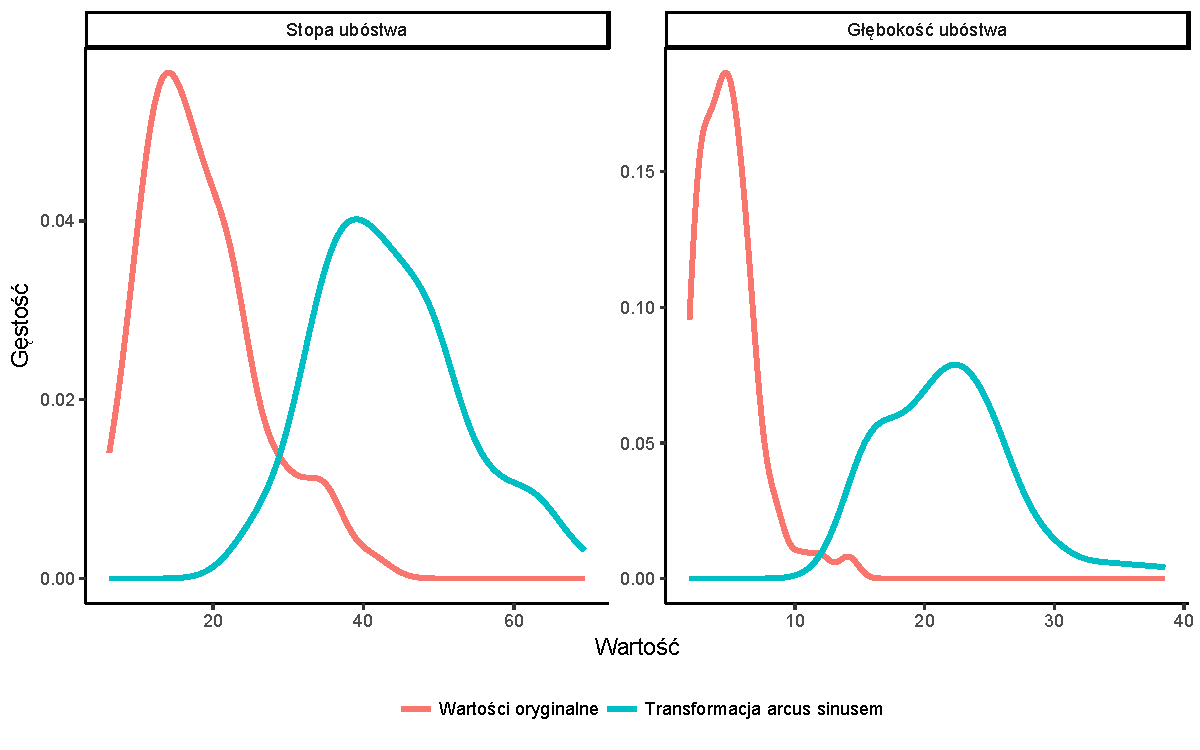
\includegraphics[width=0.8\textwidth]{04_wykresy/podreg_trans-1.pdf}
\caption{Rozkład oszacowań bezpośrednich stopy oraz głębokości ubóstwa na poziomie podregionów --- wartości oryginalne oraz transformowane z wykorzystaniem pierwiastka arcus sinusa}
\small{Źródło: opracowanie własne na podstawie badania EU-SILC 2011.}
\label{fig:podreg_trans}
\end{figure}

Zastosowana transformacja zbliżyła rozkłady obu cech do rozkładu normalnego. Zmianie uległa dyspersja analizowanych wskaźników --- współczynnik zmienności zmalał dwukrotnie, zarówno w przypadku stopy (z 42\% do 22\%), jak i głębokości ubóstwa (z 48\% do 23\%). Trzeci moment centralny oryginalnych wartości stopy ubóstwa wynosił 0,83, natomiast po transformacji wartość ta była równa 0,49. Odpowiednio dla głębokości ubóstwa skośność zmniejszyła się z 1,47 do 0,78. Zastosowana transformacja miała na celu poprawę statystyk dopasowania modelu. W przypadku liniowego modelu dla stopy ubóstwa poprawiono współczynnik $R^2$ z 69,37\% do 72,17\%. Model liniowy dla głębokości ubóstwa charakteryzował się mniejszym przyrostem współczynnika determinacji: z 54,67\% na 54,98\%.

Tak zdefiniowane zmienne zależne oraz wyspecyfikowane cechy niezależne zostały wykorzystane w klasycznym modelu Faya-Herriota oraz modelu Faya-Herriota z przestrzennie skorelowanym efektem losowym.

\subsubsection{Estymacja pośrednia stopy oraz głębokości ubóstwa z wykorzystaniem podejścia obszarowego}

Wybór najlepszego sposobu estymacji stopy oraz głębokości ubóstwa weryfikowany był na podstawie kilku kryteriów: rozkładu względnych błędów oszacowań, kryterium AIC, a także empirycznego obciążenia ocen estymatorów. Błąd średniokwadratowy wszystkich estymatorów został oszacowany z wykorzystaniem metody bootstrap o liczbie replikacji $B=500$, co zapewniło porównywalność wyników.

W celu lepszego zobrazowania przestrzennego aspektu ubóstwa zastosowano model Faya-Herriota z przestrzennie skorelowanym efektem losowym. Podejście to wymagało wyznaczenia macierzy sąsiedztwa dla podregionów w Polsce. W tradycyjnej macierzy sąsiedztwa $W^0$ elementy diagonalne są równe 0, natomiast pozostałe elementy macierzy przyjmują wartość równą 1, w przypadku gdy dwa obszary ze sobą sąsiadują, a 0 w przeciwnym razie. Macierz $W$ konieczną do zastosowania w funkcji \emph{eblupSFH}, otrzymuje się na podstawie $W^0$ poprzez podzielenie każdego elementu w wierszu przez sumę wiersza. W ten sposób uzyskuje się macierz wierszowo-standaryzowaną, której suma każdego wiersza jest równa 1.

Na rysunku \ref{fig:podreg_oszac} przedstawiono rozkład oszacowań wskaźników ubóstwa uzyskanych z~wykorzystaniem estymacji bezpośredniej oraz pośredniej.

\begin{figure}[htp]
\centering
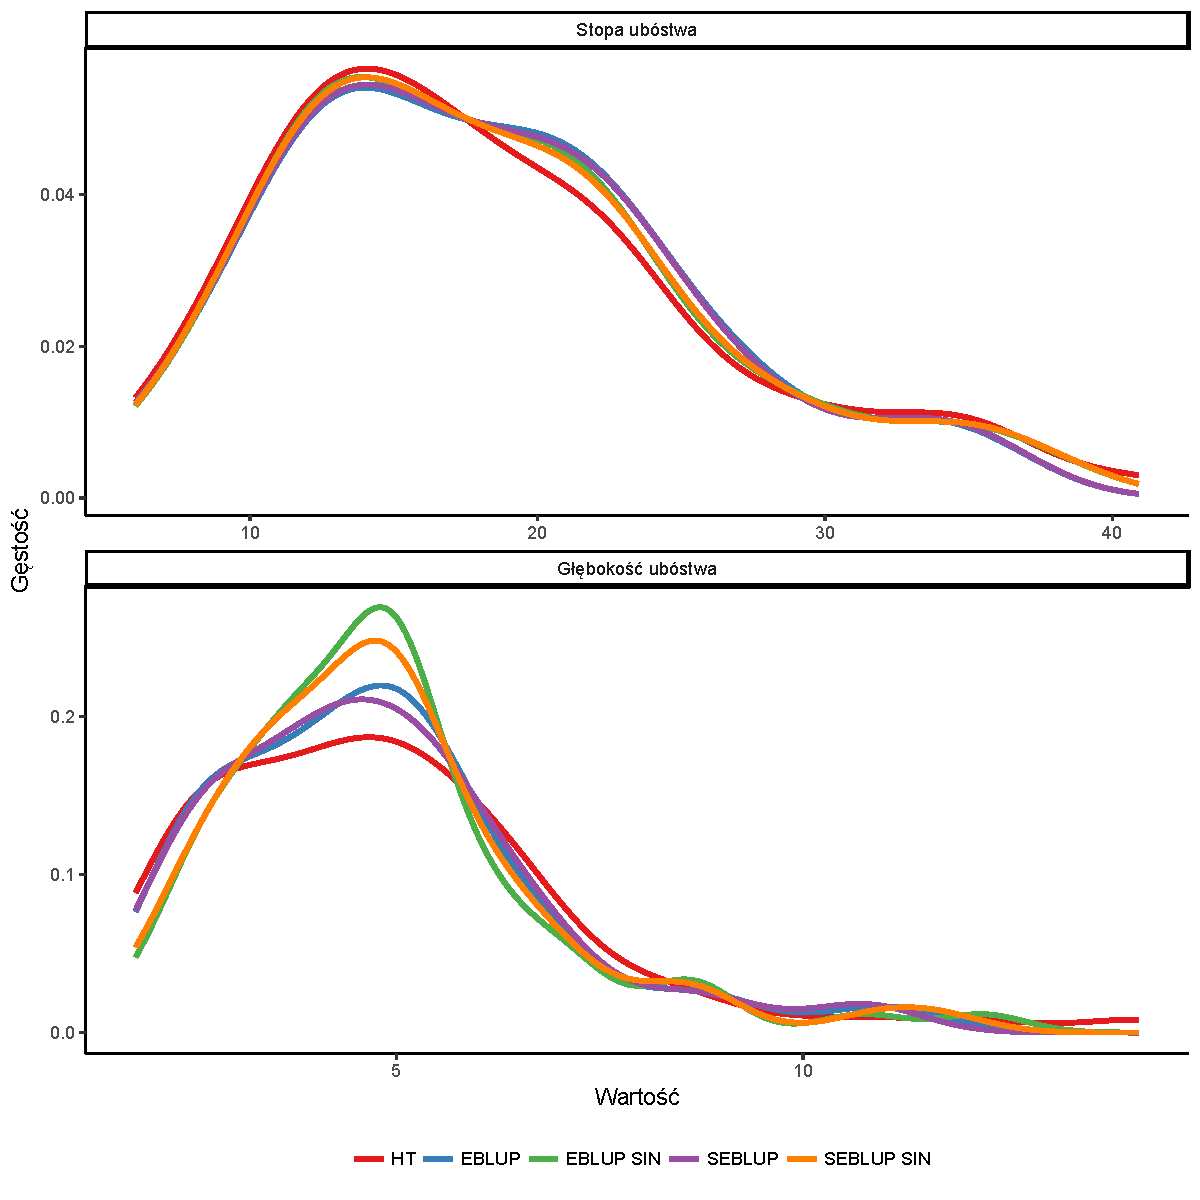
\includegraphics[width=0.8\textwidth]{04_wykresy/model_podreg_oszacowania-1.pdf}
\caption{Rozkład oszacowań bezpośrednich i pośrednich stopy oraz głębokości ubóstwa na poziomie podregionów --- wartości oryginalne oraz transformowane z wykorzystaniem pierwiastka arcus sinusa}
\small{Źródło: opracowanie własne na podstawie badania EU-SILC 2011, NSP 2011 oraz BDL.}
\label{fig:podreg_oszac}
\end{figure}

Rozkłady oszacowań stopy oraz głębokości ubóstwa są do siebie zbliżone. Średnie oszacowania stopy ubóstwa wynoszą 18\% dla wszystkich analizowanych estymatorów oraz 5\% dla głębokości ubóstwa. W przypadku drugiego z badanych wskaźników widoczne są większe rozbieżności w~rozkładach. Mediana oszacowań zarówno w przypadku stopy, jak i głębokości ubóstwa jest nieznacznie niższa od średniej.

Współczynnik korelacji przestrzennej efektów losowych w przypadku stopy ubóstwa wynosił 0,47 oraz 0,53 dla głębokości ubóstwa. Wartości te dotyczą modeli, w których zastosowano transformację zmiennej zależnej. Dla modeli wykorzystujących oryginalne wartości zmiennej $y$~otrzymano odpowiednio 0,46 i 0,41. Kryterium informacyjne Akaikego w przypadku estymacji stopy ubóstwa w modelu Faya-Herriota z przekształceniem zmiennej zależnej wynosiło -193,78, natomiast dla modelu przestrzennego -195,68. Z kolei estymacja głębokości ubóstwa charakteryzowała się mniejszą wartością kryterium AIC: -245,48 dla klasycznego modelu FH w porównaniu do wartości -246,94 dla modelu uwzględniającym korelację przestrzenną. W przypadku modeli szacowanych na podstawie nietransformowanych danych zaobserwowano analogiczną sytuację --- przewaga estymatora SEBLUP nad EBLUP dla stopy ubóstwa oraz niższe kryterium AIC dla estymatora EBLUP w sytuacji, gdy szacowana jest głębokość ubóstwa.

\subsubsection{Ocena precyzji oszacowań}

W celu oceny precyzji szacunków, mając na uwadze z jednej strony zbliżone rozkłady oszacowań wskaźników ubóstwa, zaś z drugiej niejednoznaczne oceny kryterium AIC, porównano rozkłady względnych błędów oszacowań dla poszczególnych estymatorów (por. rys. \ref{fig:podreg_prec}). Zestawienie wartości błędów otrzymanych dla różnych metod estymacji było możliwe dzięki zastosowaniu przy ich wyznaczeniu metody bootstrap.

\begin{figure}[htp]
\centering
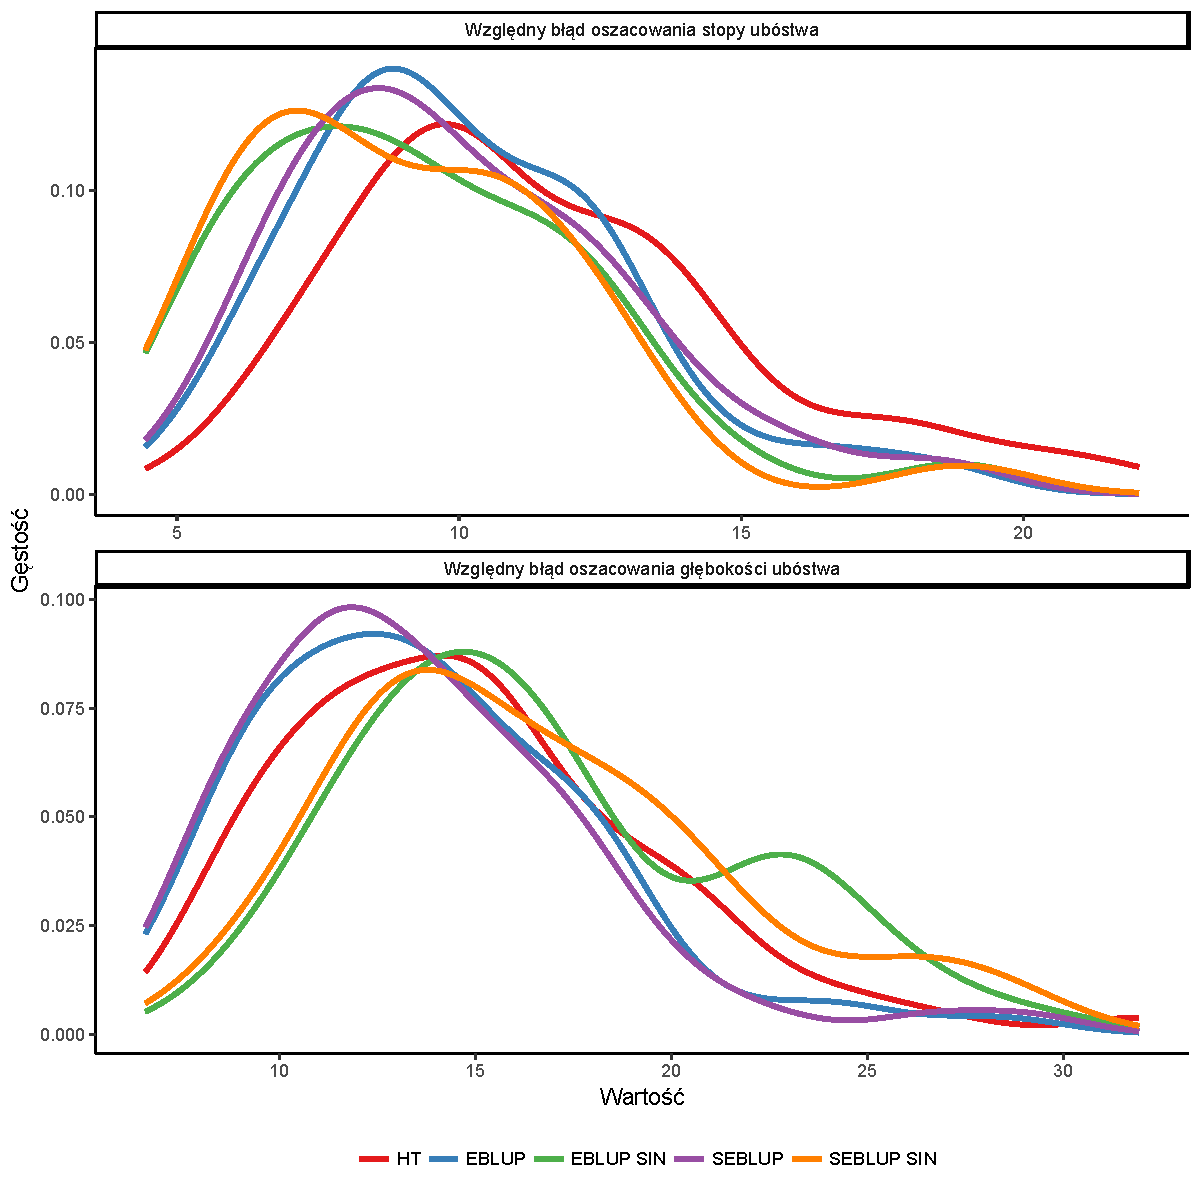
\includegraphics[width=0.8\textwidth]{04_wykresy/model_podreg_precyzja-1.pdf}
\caption{Rozkład względnych błędów oszacowań bezpośrednich i pośrednich stopy oraz głębokości ubóstwa na poziomie podregionów --- wartości oryginalne oraz transformowane z wykorzystaniem pierwiastka arcus sinusa}
\small{Źródło: opracowanie własne na podstawie badania EU-SILC 2011, NSP 2011 oraz BDL.}
\label{fig:podreg_prec}
\end{figure}

W przypadku stopy ubóstwa najniższe średnie oszacowania błędu otrzymano dla estymatora SEBLUP, w którym zastosowano transformację z wykorzystaniem pierwiastka arcus sinusa. Średni poziom tej cechy wynosił 9,11\% w porównaniu do 10,07\% dla estymatora bez transformacji zmiennej zależnej oraz 11,62\% dla oszacowań bezpośrednich. Sytuacja dla wskaźnika głębokości ubóstwa była nieco inna --- poprawę precyzji w odniesieniu do estymacji bezpośredniej obserwuje się w przypadku estymatorów EBLUP i SEBLUP bez transformacji. Natomiast oszacowania pośrednie uzyskane z zastosowaniem przekształcenia pierwiastka arcus sinusa cechują się gorszą precyzją w porównaniu do oszacowań bezpośrednich.

\subsubsection{Ocena obciążenia oszacowań}

W kolejnym kroku ocenie poddano obciążenie rezultatów. Wykorzystano w tym celu test Walda sprawdzający istotność różnic pomiędzy oszacowaniami bezpośrednimi i pośrednimi z uwzględnieniem błędów standardowych ocen szacunków. Wyniki obliczeń przedstawiono w tabeli \ref{tab:wald_podreg}.

\begin{table}[htp]
\caption{Wartości statystyki Walda dla oszacowań pośrednich stopy oraz głębokości ubóstwa na poziomie podregionów}
\label{tab:wald_podreg}
\begin{center}
\begin{tabular}{lrr}
\hline
Estymator & Stopa ubóstwa & Głębokość ubóstwa\tabularnewline
\hline
EBLUP & 12,27 & 9,33\tabularnewline
EBLUP SIN & 5,13 & 21,32\tabularnewline
SEBLUP & 12,76 & 10,75\tabularnewline
SEBLUP SIN & 6,19 & 23,22\tabularnewline
\hline
$\chi^2_{66}$ & \multicolumn{2}{c}{85,96}\tabularnewline
\hline
\end{tabular}\\
\end{center}
\small{Źródło: opracowanie własne na podstawie badania EU-SILC 2011, NSP 2011 oraz BDL.}
\end{table}

We wszystkich przypadkach wartość statystyki empirycznej była mniejsza od wartości statystyki testowej. W związku z tym nie ma podstaw do odrzucenia hipotezy zerowej zakładającej identyczność rozkładów. Zarówno w przypadku oszacowań stopy, jak i głębokości ubóstwa różnice pomiędzy oszacowaniami uzyskanymi z wykorzystaniem estymatora bezpośredniego oraz pośredniego nie różnią się między sobą istotnie statystycznie.

Ocenie poddano także empiryczne obciążenie otrzymanych oszacowań. W tym celu wykorzystano parametryczną metodę bootstrap. Rozkład względnych obciążeń empirycznych przedstawia rysunek \ref{fig:podreg_bias}.

\begin{figure}[htp]
\centering
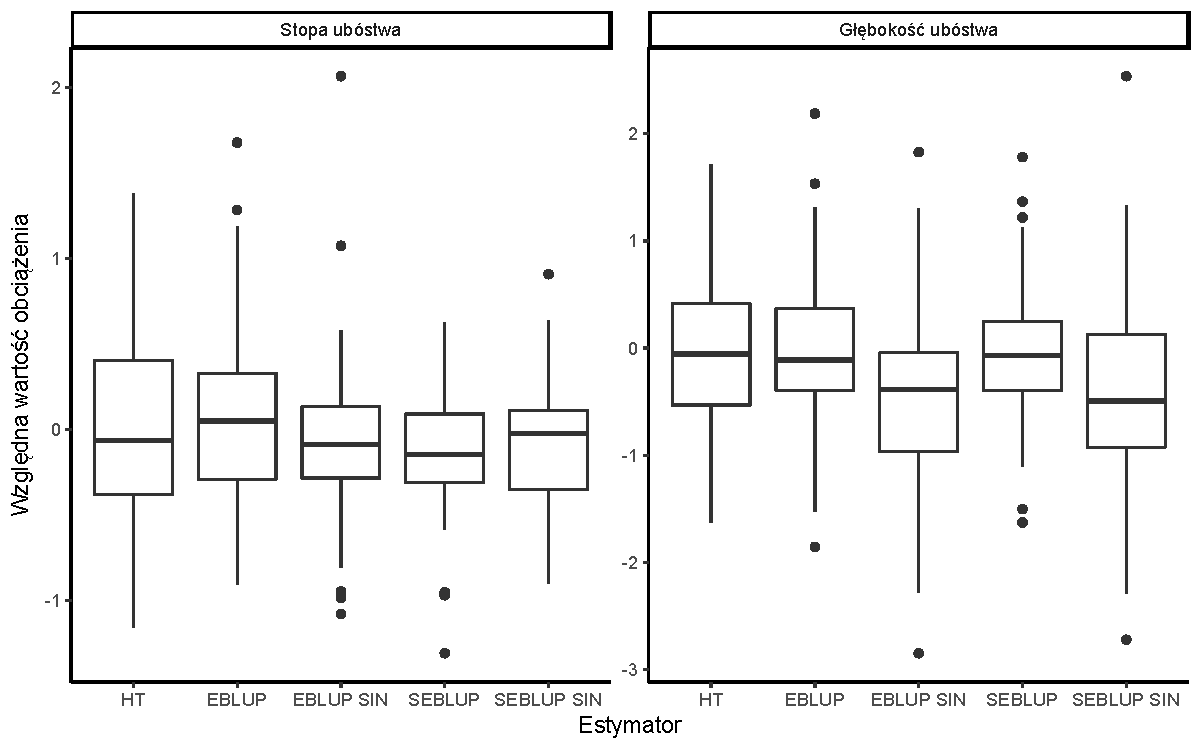
\includegraphics[width=0.8\textwidth]{04_wykresy/fh_podreg_bias-1.pdf}
\caption{Rozkład względnych obciążeń stopy oraz głębokości ubóstwa --- oszacowania bezpośrednie i pośrednie na poziomie podregionów}
\small{Źródło: opracowanie własne na podstawie badania EU-SILC 2011, NSP 2011 oraz BDL.}
\label{fig:podreg_bias}
\end{figure}

Względne empiryczne obciążenie oszacowań stopy ubóstwa dla zastosowanych estymatorów jest niewielkie i dla obu wskaźników nie przekracza 3 punktów procentowych. Miary centralne analizowanej cechy są zbliżone do zera. Jedynie względne obciążenie głębokości ubóstwa estymatorów, w których zastosowano transformacje pierwiastkiem arcus sinusa odbiegają od tego poziomu. Największe niedoszacowanie (2,85 p.p.) obserwowane jest dla estymatora głębokości ubóstwa EBLUP SIN w podregionie suwalskim, a największe przeszacowanie uzyskano w podregionie m.~Poznań (2,54\%) stosując estymator SEBLUP SIN.

Przeprowadzono także test pokrycia, który wykazał, że otrzymane oszacowania znajdują się w 95\% przedziale ufności wyznaczonym przez oszacowania bezpośrednie i pośrednie.

\subsubsection{Ocena własności modelu}

Biorąc pod uwagę wartości oszacowań, względnych błędów ocen estymatorów oraz względnego obciążenia jak optymalny estymator dla obu cech --- stopy oraz głębokości ubóstwa wybrano estymator SEBLUP. Przeprowadzone obliczenia wykazały, że transformacja zmiennej zależnej ma niewielki wpływ na końcowy rezultat, a wręcz może powodować obciążenie rezultatów. Dodatkowo za zastosowaniem oryginalnych wartości zmiennych niezależnych przemawia możliwość łatwej interpretacji współczynników $\beta$ (por. tabela \ref{tab:podreg_beta}).

\begin{table}[htp]
\centering
\caption{Parametry $\beta$ modeli objaśniających stopę oraz głębokość ubóstwa na poziomie podregionów}
\label{tab:podreg_beta}
\begin{tabular}{p{10cm}rrr}
\hline
Zmienna niezależna & $\beta$ & błąd stand. & wartość p \\
\hline
\multicolumn{4}{c}{\textbf{Stopa ubóstwa}}                \\
\hline
Stała   & 0,9033 & 0,2079 & 0,0000 \\
Udział osób niepełnosprawnych prawnie w liczbie ludności ogółem & 1.2933 & 0.3260 & 0.0000\\
Udział rodzin z 3 dzieci poniżej 24 roku życia pozostających na utrzymaniu & 1.1636 & 0,2522 & 0.0000 \\
Gęstość zaludnienia (zmienna binarna) & 0.0390 & 0.0105 & 0.0002 \\
Odsetek mieszkań posiadających ustęp spłukiwany & -0.9871 & 0.2030 & 0.0000 \\
\hline
\multicolumn{4}{c}{\textbf{Głębokość ubóstwa}}            \\
\hline
Stała & -0.0085 & 0.0269 & 0.7520 \\
Udział mieszkań, gdzie przypada powyżej 3 osób na izbę w ogólnej liczbie mieszkań & 0.6498 & 0.2619 & 0.0131 \\
Udział osób w wieku 20--29 lat pozostających na utrzymaniu & 0.2788 & 0.0948 & 0.0033\\
Udział dzieci w wieku do lat 17, na które rodzice otrzymują zasiłek rodzinny & 0.0014 & 0.0005 & 0.0025 \\
Przeciętna liczba osób w gospodarstwie domowym & -0.0250 & 0.0099 & 0.0115 \\
Stopa bezrobocia rejestrowanego osób pozostających bez pracy powyżej 12 miesięcy & -0.2982 & 0.1177 & 0.0113 \\
\hline
\end{tabular}\\
\small{Źródło: opracowanie własne na podstawie badania EU-SILC 2011, NSP 2011 oraz BDL.}
\end{table}

Wśród parametrów $\beta$ oszacowanych dla modelu opisującego stopę ubóstwa, trzy z czterech są dodatnie, co oznacza, że wzrost udziału osób niepełnosprawnych prawnie w liczbie ludności ogółem w podregionie oraz wzrost udziału rodzin z 3 dzieci poniżej 24 roku życia pozostających na utrzymaniu w liczbie rodzin z dziećmi poniżej 24 roku życia w podregionie wpływa także na wzrost stopy ubóstwa. Wyższe wartości stopy ubóstwa będą także obserwowane w podregionach o mniejszej gęstości zaludnienia. Przeciętnie w podregionach o wyższym odsetku mieszkań posiadających ustęp spłukiwany występuje także niższa stopa ubóstwa. Na wielkość głębokości ubóstwa dodatni wpływ mają takie cechy jak udział mieszkań, gdzie przypada powyżej 3 osób na izbę w ogólnej liczbie mieszkań, udział osób w wieku 20 - 29 lat pozostających na utrzymaniu w ogólnej liczbie osób w wieku 20-29 lat oraz udział dzieci w wieku do lat 17, na które rodzice otrzymują zasiłek rodzinny w ogólnej liczbie dzieci w tym wieku. Wzrost przeciętnej liczby osób w gospodarstwie domowym lub stopy bezrobocia rejestrowanego osób pozostających bez pracy powyżej 12 miesięcy wpływa na zmniejszenie wartości głębokości ubóstwa. Wszystkie parametry $\beta$ są istotne, a pomiędzy zmiennymi nie występuje współliniowość o czym świadczą niskie wartości współczynników $VIF$.

Wartości parametru $\hat{\gamma}$ wskazującego jaką część końcowego oszacowania ma stanowić oszacowanie bezpośrednie i regresyjne w przypadku stopy ubóstwa należały do przedziału {[}0,48--0,93{]} z~medianą równą 0,76. Oznacza to, że dla połowy podregionów oszacowanie bezpośrednie stanowiło co najmniej 76\% końcowego oszacowania. Podregionem dla którego przyjęto 93\% oszacowania bezpośredniego było m. st. Warszawa, natomiast dla podregionu gorzowskiego estymator bezpośredni stanowił tylko 48\% końcowego oszacowania. Podregion gorzowski charakteryzował się najwyższa wartością błędu standardowego szacunku bezpośredniego. 

Z kolei przy estymacji głębokości ubóstwa parametr $\hat{\gamma}$ przyjmował wartości z przedziału {[}0,13--0,70{]}, a mediana była na poziomie 0,34. Ta wartość oznacza niską precyzję oszacowań bezpośrednich głębokości ubóstwa, które w większości przypadków miały mniejszy udział w ostatecznym oszacowaniu. Analogicznie jak w przypadku stopy ubóstwa, dla tych samych podregionów otrzymano skrajne wartości parametru $\hat{\gamma}$.

Kolejnym krokiem w analizie było zweryfikowanie założenia modelu dotyczącego normalności reszt oraz efektów losowych. Na rysunku \ref{fig:podreg_model_r} zestawiono wartości reszt standaryzowanych oraz oszacowań uzyskanych z wykorzystaniem estymatora SEBLUP. Ponadto zastosowano test Kołomogorowa-Smirnowa (KS) w celu weryfikacji zgodności rozkładów.

\begin{figure}[htp]
\centering
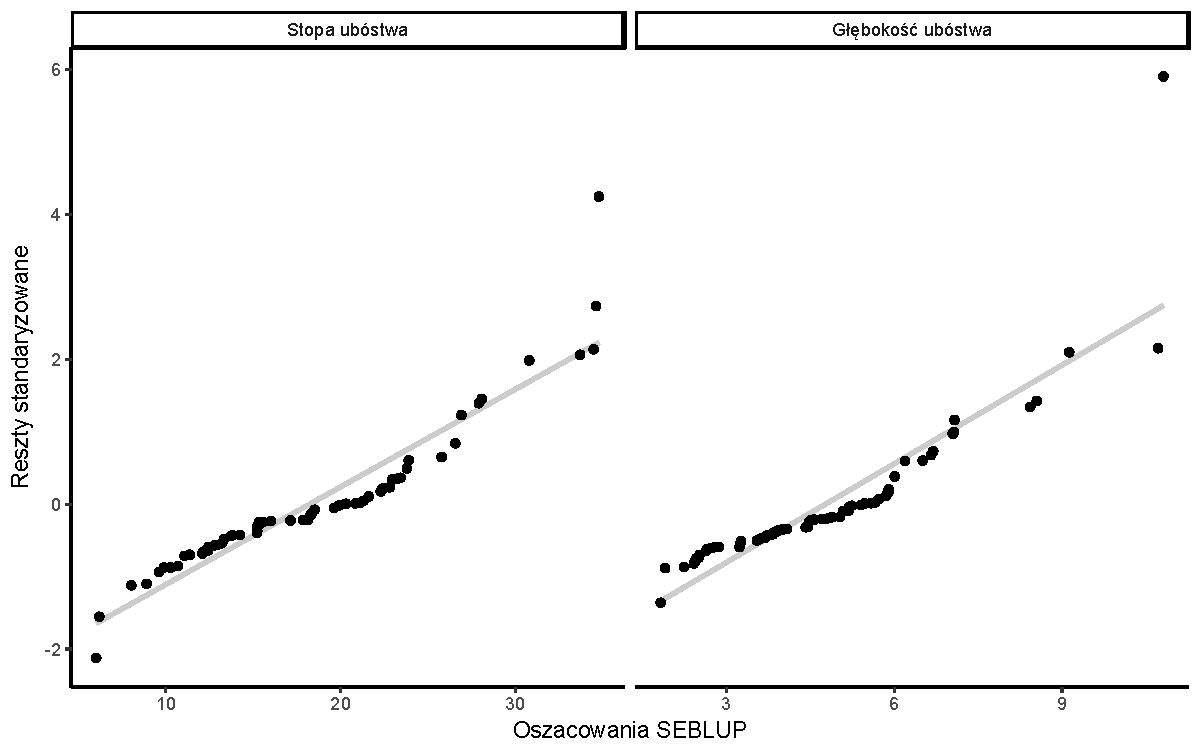
\includegraphics[width=0.8\textwidth]{04_wykresy/fh_podreg_r_model-1.pdf}
\caption{Porównanie reszt standaryzowanych i oszacowań stopy oraz głębokości ubóstwa na poziomie podregionów}
\small{Źródło: opracowanie własne na podstawie badania EU-SILC 2011, NSP 2011 oraz BDL.}
\label{fig:podreg_model_r}
\end{figure}

Na rysunku \ref{fig:podreg_model_r} można zidentyfikować kilka obserwacji odstających --- tzn. takich, dla których wartość reszty standaryzowanej jest większa od 3. W przypadku stopy ubóstwa był to podregion gorzowski oraz tarnowski, natomiast dla głębokości ubóstwa wysokie wartości reszt odnotowano dla podregionu sandomiersko-jędrzejowskiego oraz nowosądeckiego. Oszacowania wskaźników ubóstwa w tych podregionach zaliczyć można do najwyższych. Pomimo tego, w obu przypadkach nie ma podstaw do odrzucenia hipotezy o normalności rozkładu w teście Kołmogorowa-Smirnowa, przyjmując poziom $\alpha=0,05$. Wartość p w teście dla reszt oszacowań stopy ubóstwa była równa 0,2264, natomiast w przypadku głębokości ubóstwa wynosiła 0,0659.

Następnie poddano weryfikacji hipotezę o normalności efektów losowych. Na rysunku \ref{fig:podreg_model_u} przedstawiony jest wykres kwantyl-kwantyl.

\begin{figure}[htp]
\centering
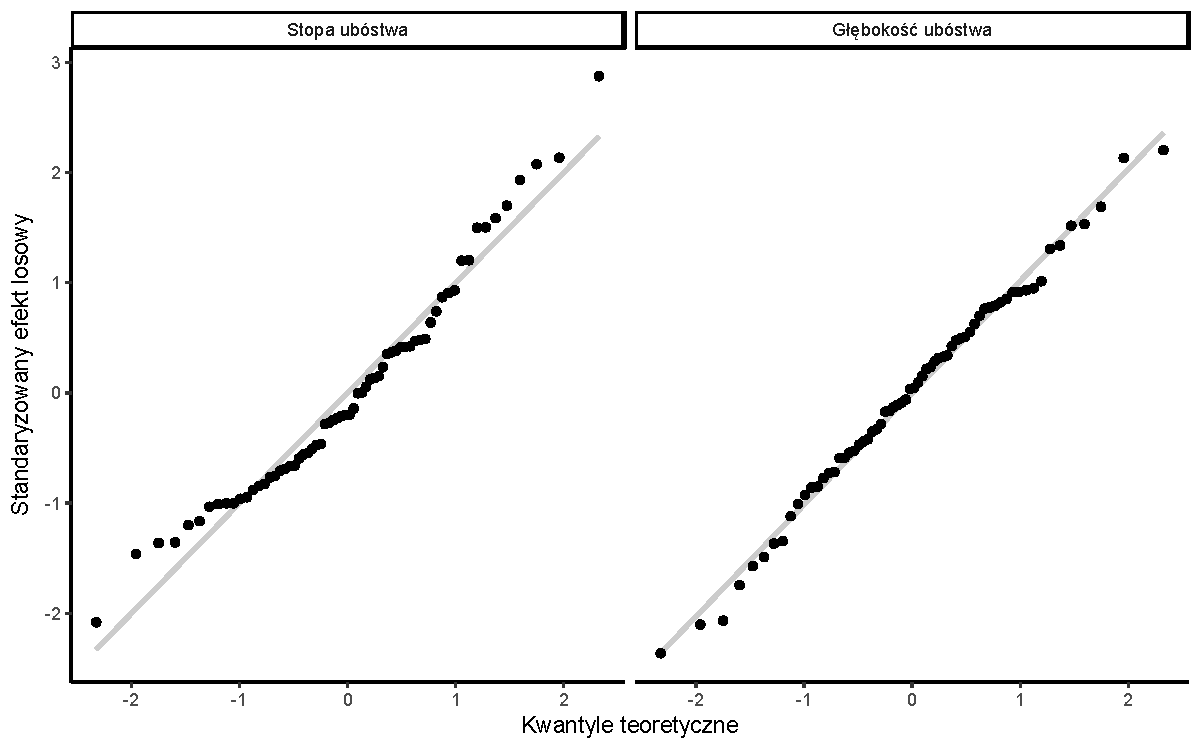
\includegraphics[width=0.8\textwidth]{04_wykresy/fh_podreg_u_model-1.pdf}
\caption{Porównanie kwantyli efektów losowych i kwantyli rozkładu
normalnego stopy oraz głębokości ubóstwa na poziomie podregionów}
\small{Źródło: opracowanie własne na podstawie badania EU-SILC 2011, NSP 2011 oraz BDL.}
\label{fig:podreg_model_u}
\end{figure}

Efekty losowe dla podregionów nieznacznie odbiegają od rozkładu normalnego --- nie zidentyfikowano wartości odstających, a w teście Kołmogorowa-Smirnowa nie ma podstaw do odrzucenia hipotezy zerowej. Wartość p dla obu wskaźników wynosiła 0,9505. Wyżej przeprowadzona weryfikacja modelu wskazuje, że są spełnione założenia, a w związku z tym dobrany model jest poprawny.

Oszacowania otrzymane z wykorzystaniem przestrzennego modelu Faya-Herriota charakteryzują się lepszą precyzją w porównaniu do estymacji bezpośredniej. W tabeli \ref{tab:podreg_prec} zestawiono częstości względnych błędów standardowych oszacowań.

\begin{table}[htp]
\caption{Porównanie precyzji oszacowań bezpośrednich oraz pośrednich stopy oraz głębokości ubóstwa na poziomie podregionów}
\label{tab:podreg_prec}
\centering
\begin{tabular}{lrrrr}
\hline
Wartość RRMSE & $F_0$ HT & $F_0$ SEBLUP & $F_1$ HT & $F_1$ SEBLUP\tabularnewline
\hline
{[}0\%--10\%{]} & 26 & 38 & 9 & 14\tabularnewline
(10\%--20\%{]} & 37 & 28 & 47 & 48\tabularnewline
(20\%--30\%{]} & 3 & 0 & 9 & 4\tabularnewline
(30\%--40\%{]} & 0 & 0 & 1 & 0\tabularnewline
\hline
\end{tabular}\\
\small{Źródło: opracowanie własne na podstawie badania EU-SILC 2011, NSP 2011 oraz BDL.}
\end{table}

Grupując wskaźniki precyzji w przedziały klasowe o rozpiętości 10 punktów procentowych można ocenić skalę poprawy jakości estymacji pośredniej w odniesieniu do estymacji bezpośredniej. W przypadku stopy ubóstwa w przedziale do 10\% znalazło się 58\% podregionów podczas gdy estymacja bezpośrednia umożliwiła taką precyzję tylko dla 26 podregionów. Wartościami w przedziale od 10 do 20 procent cechowało się pozostałe 42\% analizowanych jednostek terytorialnych. W przypadku głębokości ubóstwa zmiany liczebności obserwowane są we wszystkich przedziałach klasowych z wyjątkiem drugiego --- od 10\% do 20\%. W pierwszym przedziale klasowym dla estymatora SEBLUP znalazło się o pięć podregionów więcej w porównaniu do estymatora Horvitza-Thompsona. Jednostek z największym błędem szacunku jest z kolei mniej --- względny błąd oszacowania głębokości ubóstwa dla żadnej jednostki nie przekracza 30\%. Takie rezultaty można uznać za bardzo dobre, zwłaszcza, że GUS za granicę dopuszczającą możliwość publikacji bez tworzenia dodatkowych agregatów przyjmuje wartość RRMSE równą 20\%.

Precyzja oszacowań uzależniona była w dużej mierze od liczby reprezentantów osób ubogich w podregionie. Współczynnik korelacji wskaźnika precyzji i liczby reprezentantów był wysoki i wynosił $r=-0,84$ w przypadku stopy ubóstwa oraz $r=-0,82$ w przypadku głębokości ubóstwa. Stąd też małym błędem oszacowania cechowały się podregiony o dużej liczebności: podregion chełmsko-zamojski, tarnowski oraz puławski. Z kolei najmniej reprezentantów ubogich odnotowano w Poznaniu oraz Wrocławiu, co przełożyło się na wyższy względny błąd oszacowania.

\subsection{Poziom powiatów}

Kolejnym etapem prac nad estymacją stopy oraz głębokości ubóstwa w Polsce była próba oszacowania wskaźników ubóstwa na poziomie powiatów. Powiat ma tę przewagę nad podregionem, że poza jednostką statystyczną jest również jednostką administracyjną. Dzięki temu rezultaty prowadzonych prac mogą być wykorzystywane przez władze powiatów przy planowaniu chociażby polityki społecznej. W analizowanym 2011 roku w Polsce znajdowało się 379 powiatów, w tym 65 miast na prawach powiatu.

Spośród 379 powiatów Polski, cztery nie były w ogóle reprezentowane w próbie badania EU-SILC: wieruszowski (woj. łódzkie), proszowicki (woj. małopolskie), moniecki (woj. podlaskie), włoszczowski (woj. świętokrzyskie). Ponadto, w kolejnych 12 powiatach nie znalazło się żadne ubogie gospodarstwo, co uniemożliwiało uzyskanie szacunków z wykorzystaniem estymatora Horvitza-Thompsona. W związku z tym w analizie rozpatrywano 363 powiaty, dla których udało się oszacować stopę oraz głębokość ubóstwa.

\subsubsection{Estymacja pośrednia stopy oraz głębokości ubóstwa z wykorzystaniem podejścia obszarowego}

Podobnie jak w przypadku wskaźników ubóstwa na poziomie podregionów, w pierwszej kolejności sprawdzono w jaki sposób transformacja z wykorzystaniem pierwiastka arcus sinusa wpływa na rozkład analizowanych cech (por. rysunek \ref{fig:pow_trans}).

\begin{figure}[htp]
\centering
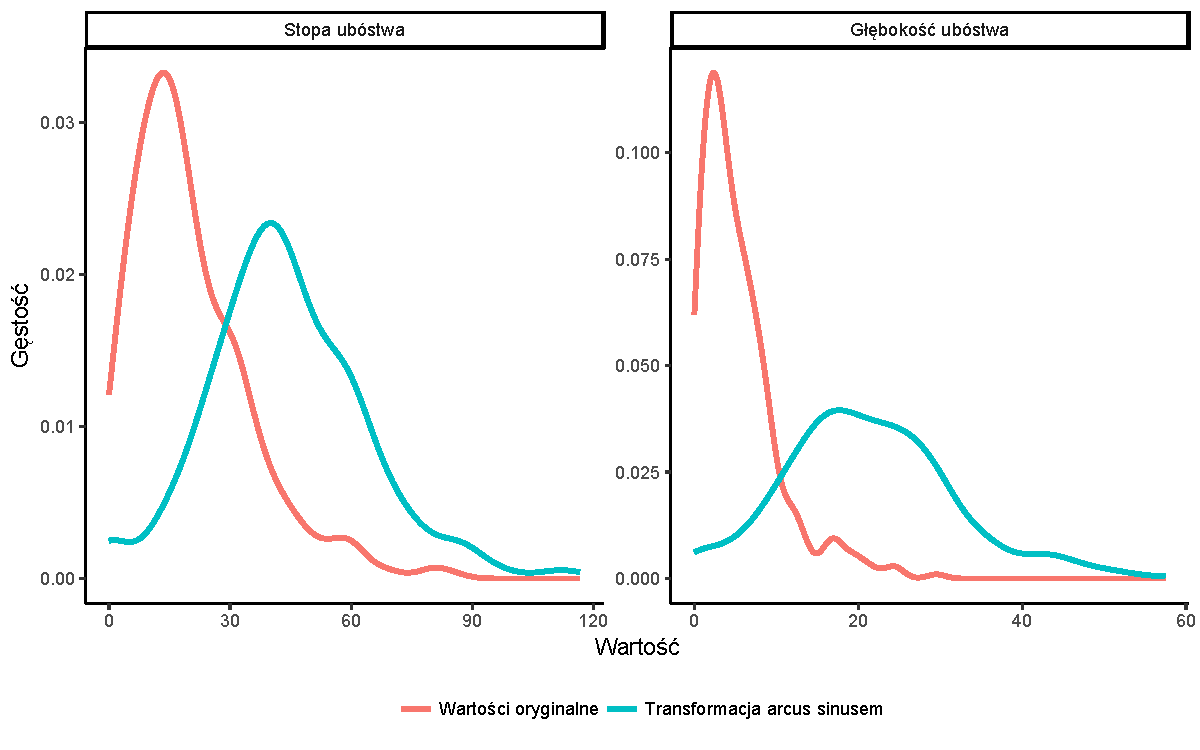
\includegraphics[width=0.8\textwidth]{04_wykresy/pow_trans-1.pdf}
\caption{Rozkład oszacowań bezpośrednich stopy oraz głębokości ubóstwa na poziomie powiatów --- wartości oryginalne oraz transformowane z wykorzystaniem pierwiastka arcus sinusa}
\small{Źródło: opracowanie własne na podstawie badania EU-SILC 2011.}
\label{fig:pow_trans}
\end{figure}

Rozkład bezpośrednich oszacowań stopy oraz głębokości ubóstwa charakteryzował się asymetrią prawostronną --- współczynnik asymetrii wynosi odpowiednio 1,3 i 1,73. Zaobserwowano także bardzo dużą dyspersję wartości wskaźników: 74\% w przypadku stopy ubóstwa oraz 89\% dla głębokości. Wynika to z faktu, że w zbiorze wartości występują oszacowania stopy ubóstwa m.in. na poziomie 84\% spowodowane dominacją reprezentantów osób ubogich w nielicznej próbie. Zastosowanie transformacji umożliwiło zmniejszenie skośności rozkładów --- stopy ubóstwa do wartości współczynnika równej 0,44 oraz głębokości ubóstwa do 0,45. Poprawie uległ także współczynnik zmienności przyjmując wartości odpowiednio 45\% oraz 49\%.

W modelu opracowanym na potrzeby estymacji stopy ubóstwa znalazły się następujące zmienne: udział osób niepełnosprawnych prawnie w liczbie ludności w powiecie, wskaźnik zależności osób w wieku poprodukcyjnym w odniesieniu do liczby osób w wieku produkcyjnym, odsetek osób samotnych powyżej 25 roku życia, udział osób utrzymujących się z~pracy w~rolnictwie w~ogólnej liczbie ludności, wskaźnik zatrudnienia w powiecie, odsetek rodzin z dziećmi do 24 roku życia pozostających na utrzymaniu. Z kolei zmienność głębokości ubóstwa wyjaśniana jest przez udział osób utrzymujących się z pracy w rolnictwie w ogólnej liczbie ludności, odsetek osób samotnych powyżej 25 roku życia, udział osób w wieku 20--29 lat pozostających na utrzymaniu w liczbie osób w wieku 20--29 lat, odsetek gospodarstw zamieszkiwanych przez 4 osoby w liczbie gospodarstw w powiecie, udział osób niepełnosprawnych prawnie w liczbie osób niepełnosprawnych w~powiecie oraz odsetek osób w wieku 20--64 lat posiadających wykształcenie zawodowe (logarytm naturalny).

\begin{figure}[htp]
\centering
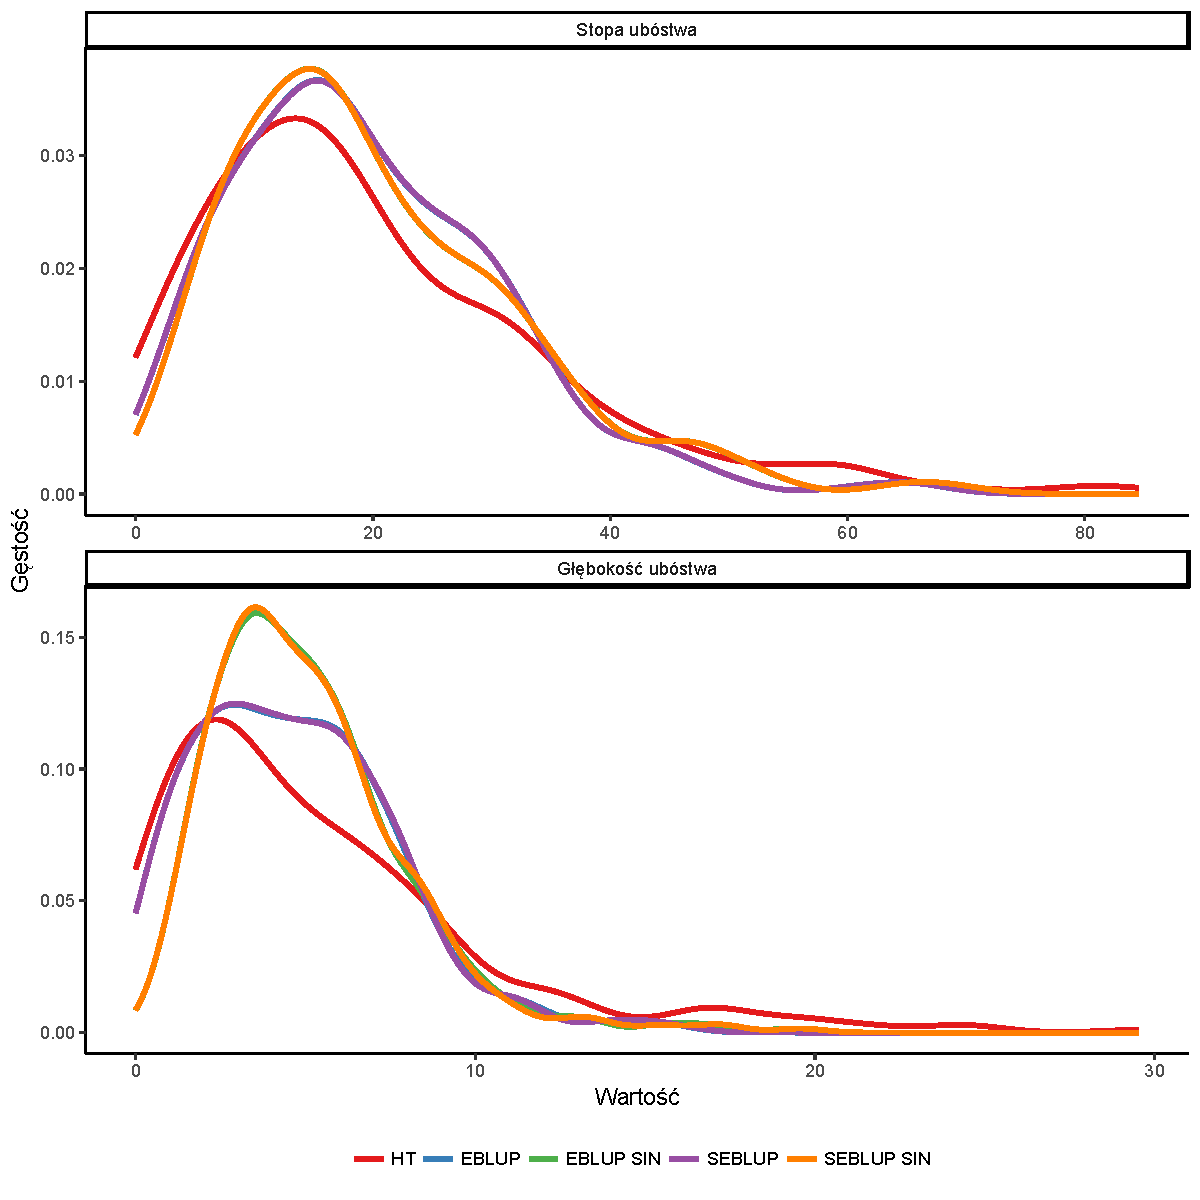
\includegraphics[width=0.8\textwidth]{04_wykresy/fh_powiat-1.pdf}
\caption{Rozkład oszacowań bezpośrednich i pośrednich stopy oraz głębokości ubóstwa na poziomie powiatów --- wartości oryginalne oraz transformowane z wykorzystaniem pierwiastka arcus sinusa}
\small{Źródło: opracowanie własne na podstawie badania EU-SILC 2011, NSP 2011 oraz BDL.}
\label{fig:fh_powiat}
\end{figure}

Oszacowania stopy oraz głębokości ubóstwa uzyskane z wykorzystaniem estymatorów EBLUP i SEBLUP oraz EBLUP i SEBLUP z zastosowaniem transformacji cechują się bardzo zbliżonym rozkładem --- linie opisujące rozkład oszacowań w zasadzie się pokrywają (por. rys. \ref{fig:fh_powiat}). Mediana oszacowań jest równa 17\% dla stopy ubóstwa oraz 4\% dla głębokości. Zastosowanie estymatorów pośrednich powinno przyczynić się do zmniejszenia rozstępu, a tym samym dyspersji estymowanej cechy. Tymczasem maksymalna wartość stopy ubóstwa uzyskana metodami estymacji pośredniej wynosiła 70\%, a głębokości ubóstwa 20\%. Oznacza to, że zmienność oszacowań stopy ubóstwa zmalała z 74\% do 60\%, a oszacowań głębokości ubóstwa z 89\% do 55\%. Z literatury przedmiotu wiadomo, że estymatory obszarowe są przykładem estymatorów ,,kurczących'', co znaczy, że rozstęp oszacowań pośrednich będzie mniejszy od rozstępu oszacowań bezpośrednich \citep{chakraborty2016,rao2015}.

Współczynnik $R^2$ dla modelu liniowego objaśniającego stopę ubóstwa wynosił 25\%, a dla głębokości ubóstwa 20\%. Kryterium informacyjne Akaikego dla estymatora EBLUP w przypadku estymacji stopy ubóstwa wynosiło -507,55, a dla estymatora SEBLUP -505,81. Po zastosowaniu transformacji zmiennej zależnej, model z przestrzennym efektem losowym nadal charakteryzował się wyższą wartością kryterium AIC w porównaniu do klasycznego modelu Faya-Herriota. Przyczyną takiego stanu rzeczy mogły być niskie współczynniki autokorelacji przestrzennej wynoszące $\rho=-0,03$ dla stopy ubóstwa oraz $\rho=0,10$ dla głębokości ubóstwa.

\subsubsection{Ocena precyzji}

Oceny precyzji szacunków dokonano porównując względne błędy oszacowań dla poszczególnych estymatorów (por. rys. \ref{fig:fh_powiat_prec}). 

\begin{figure}[htp]
\centering
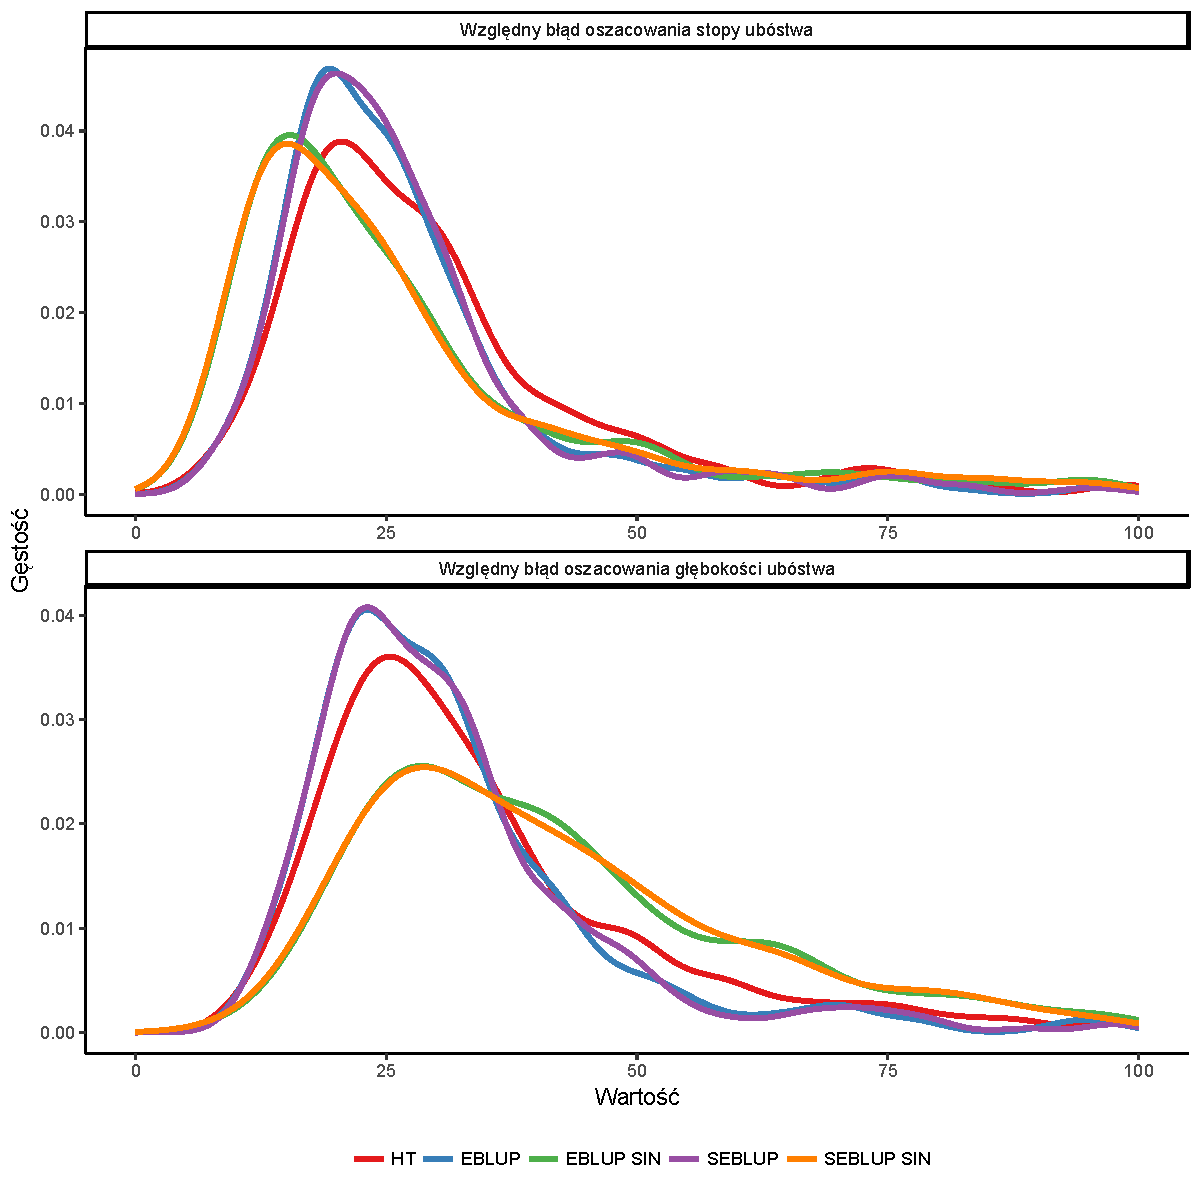
\includegraphics[width=0.8\textwidth]{04_wykresy/fh_pow_prec-1.pdf}
\caption{Rozkład względnych błędów oszacowań bezpośrednich i pośrednich stopy oraz głębokości ubóstwa na poziomie powiatów --- wartości oryginalne oraz transformowane z wykorzystaniem pierwiastka arcus sinusa}
\small{Źródło: opracowanie własne na podstawie badania EU-SILC 2011, NSP 2011 oraz BDL.}
\label{fig:fh_powiat_prec}
\end{figure}

Rozkłady względnych błędów oszacowań wskaźników ubóstwa różnią się w zależności od zastosowanej metody i przekształcenia zmiennej zależnej. W analizowanym przypadku, w którym rozkład wskaźnika precyzji jest asymetryczny, analizę struktury przeprowadzono bazując na miarach pozycyjnych. W przypadku stopy ubóstwa najniższą medianą (22\%) charakteryzowały się oszacowania uzyskane na podstawie transformowanej wartości wskaźnika. Dla estymatorów EBLUP i SEBLUP mediana była wyższa, wynosiła 24\%, ale nadal była to wartość, która wskazywała na większą precyzję podejść pośrednich w porównaniu do estymacji bezpośredniej, gdzie RRMSE wynosił 26\%. Wartości pozostałych miar pozycyjnych charakteryzowały takie same relacje. Z~kolei średnia wartość względnego błędu szacunku dla estymatora bezpośredniego wynosiła 30\%, a~dla estymacji pośredniej była nieco wyższa i wynosiła 33\%--34\%. Świadczy to o tym, że zastosowanie metod pośrednich wpłynęło na nieznaczne pogorszenie przeciętnej precyzji. Należy jednak pamiętać o wadach tej miary tendencji centralnej w przypadku rozkładów asymetrycznych.

\subsubsection{Ocena obciążenia}

Za pomocą testu Walda sprawdzono istotność różnic pomiędzy oszacowaniami pośrednimi oraz bezpośrednimi. Wyniki przedstawiono w tabeli \ref{tab:wald_pow}.

\begin{table}[htp]
\caption{Wartości statystyki Walda dla oszacowań pośrednich stopy oraz głębokości ubóstwa na poziomie powiatów --- podejście obszarowe}
\label{tab:wald_pow}
\centering
\begin{tabular}{lrr}
\hline
Estymator & Stopa ubóstwa & Głębokość ubóstwa\tabularnewline
\hline
EBLUP & 58,83 & 113,13\tabularnewline
EBLUP SIN & 34,74 & 167,96\tabularnewline
SEBLUP & 58,53 & 114,49\tabularnewline
SEBLUP SIN & 34,58 & 168,82\tabularnewline
\hline
$\chi^2_{364}$ & \multicolumn{2}{c}{409,49}\tabularnewline
\hline
\end{tabular}\\
\small{Źródło: opracowanie własne na podstawie badania EU-SILC 2011, NSP 2011 oraz BDL.}
\end{table}

Porównanie statystyk testowych z wartością krytyczną wskazuje, że oszacowania pośrednie są równe co do wartości oczekiwanej, oszacowaniom bezpośrednim. Test pokrycia wykazał, że skonstruowany 95\% przedział ufności nie objął tylko jednej wartości oszacowania stopy ubóstwa i czterech wartości oceny estymatora dla głębokości ubóstwa. 

Następnie ocenie poddano także empiryczne obciążenie otrzymanych oszacowań. Rozkład względnych obciążeń empirycznych przedstawiony jest na rysunku \ref{fig:fh_pow_bias}.

\begin{figure}[htp]
\centering
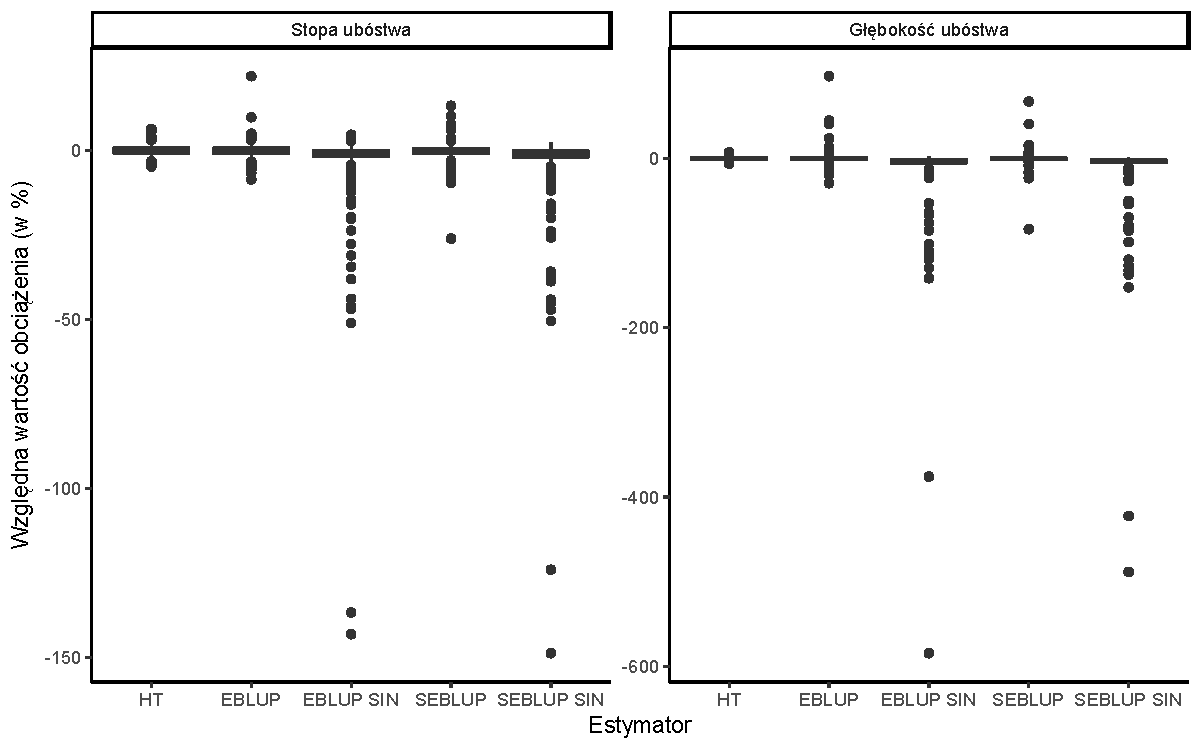
\includegraphics[width=0.8\textwidth]{04_wykresy/fh_pow_bias-1.pdf}
\caption{Rozkład względnych obciążeń stopy oraz głębokości ubóstwa --- oszacowania bezpośrednie i pośrednie na poziomie powiatów}
\small{Źródło: opracowanie własne na podstawie badania EU-SILC 2011, NSP 2011 oraz BDL.}
\label{fig:fh_pow_bias}
\end{figure}

Największe względne obciążenie oszacowań jest obserwowane w przypadku estymatorów, w~których zastosowano transformowaną zmienną zależną. Dla tych estymatorów obserwuje się średnie przeszacowanie na poziomie trzech punktów procentowych w przypadku stopy ubóstwa oraz około dziewięciu punktów procentowych w przypadku głębokości ubóstwa. Z kolei estymatory EBLUP oraz SEBLUP zastosowane na oryginalnych danych charakteryzują się przeciętnym poziomem względnego obciążenia zbliżonym do zera. Zastosowanie transformacji zmiennej doprowadziło do sytuacji, w której udział obciążenia w wartości oszacowania stanowił ponad 100\% oceny estymatora. Najmniejszym rozstępem obciążenia, spośród estymatorów pośrednich, cechował się estymator SEBLUP, w związku z czym został wybrany do dalszej analizy.

Wartości parametru $\hat{\gamma}$ wskazującego jaką część końcowego oszacowania stanowi oszacowanie bezpośrednie i regresyjne w przypadku stopy ubóstwa znajdowały się w przedziale {[}0,15--0,99{]} z~medianą równą 0,85. Oznacza to, że dla połowy powiatów oszacowanie bezpośrednie stanowiło co najmniej 85\% końcowego oszacowania. Z kolei podczas estymacji głębokości ubóstwa parametr $\hat{\gamma}$ przyjmował wartości z przedziału {[}0,01--0,96{]}, a mediana była na poziomie 0,29. Wartości parametru $\hat{\gamma}$ bliskie 1 występują w przypadku powiatów, które charakteryzowały się małym błędem oszacowania --- wówczas estymacja bezpośrednia była uznawana za odpowiednio precyzyjną.

\subsubsection{Ocena własności modelu}

W tabeli \ref{tab:pow_beta} zestawiono parametry $\beta$ wypracowanego modelu.

\begin{table}[htp]
\centering
\caption{Parametry $\beta$ modeli objaśniających stopę oraz głębokość ubóstwa na poziomie powiatów}
\label{tab:pow_beta}
\begin{tabular}{p{10cm}rrr}
\hline
Zmienna niezależna & $\beta$ & błąd stand. & wartość p \\
\hline
\multicolumn{4}{c}{\textbf{Stopa ubóstwa}}                \\
\hline
Stała & -0,7075 & 0,2918 & 0,0153 \\
Odsetek osób samotnych powyżej 25 roku życia & 1,6090 & 0,4108 & 0,0001 \\
Udział osób utrzymujących się z pracy w rolnictwie & 1,3475 & 0,2034 & 0,0000 \\
Odsetek rodzin z dziećmi do 24 roku życia pozostających na utrzymaniu & 1,0213 & 0,3194 & 0,0014 \\
Wskaźnik zależności osób w wieku poprodukcyjnym w odniesieniu do liczby osób w wieku produkcyjnym & 0,6426 & 0,2904 & 0,0269 \\
Udział osób niepełnosprawnych prawnie w liczbie ludności & 0,6389 & 0,2770 & 0,0211 \\
Wskaźnik zatrudnienia & -0,5523 & 0,1697 & 0,0011 \\
\hline
\multicolumn{4}{c}{\textbf{Głębokość ubóstwa}}            \\
\hline
Stała & 0,0150 & 0,0391 & 0,7005 \\
Odsetek osób samotnych powyżej 25 roku życia & 0,2519 & 0,1198 & 0,0354 \\
Udział osób utrzymujących się z pracy w rolnictwie & 0,2366 & 0,0583 & 0,0001 \\
Udział osób w wieku 20--29 lat pozostających na utrzymaniu w liczbie osób w wieku 20--29 lat & 0,1858 & 0,0464 & 0,0001 \\
Udział osób niepełnosprawnych prawnie w liczbie osób niepełnosprawnych & 0,0346 & 0,0233 & 0,1377 \\
Odsetek osób w wieku 20--64 lat posiadających wykształcenie zawodowe (logarytm) & 0,0349 & 0,0098 & 0,0004 \\
Odsetek gospodarstw zamieszkiwanych przez 4 osoby & -0,3176 & 0,1008 & 0,0017 \\
\hline
\end{tabular}\\
\small{Źródło: opracowanie własne na podstawie badania EU-SILC 2011, NSP 2011 oraz BDL.}
\end{table}

W modelu dla stopy ubóstwa na poziomie powiatów jedynie wskaźnik zatrudnienia wpływa na spadek zasięgu ubóstwa w powiecie. Pozostałe zmienne niezależne powodują wzrost wartości wskaźnika ubóstwa. W przypadku modelowania głębokości ubóstwa ujemny znak przy parametrze $\beta$ znajduje się tylko przy zmiennej odsetek gospodarstw zamieszkiwanych przez 4 osoby. Dwie cechy są wspólne dla obu analizowanych wskaźników: odsetek osób samotnych powyżej 25 roku życia oraz udział osób utrzymujących się z pracy w rolnictwie. W obu modelach znalazła się także cecha dotycząca odsetka osób niepełnosprawnych prawnie. Dla stopy ubóstwa jest to udział osób niepełnosprawnych prawnie w liczbie ludności ogółem, a dla głębokości ubóstwa mianownikiem tego wskaźnika jest liczba osób niepełnosprawnych ogółem. Kolejną cechą wspólną modeli jest zmienna przechowująca informację na temat pozostawania na utrzymaniu. Wszystkie zmienne niezależne są istotne oraz nie występuje zjawisko współliniowości, co potwierdzają niskie wartości współczynnika $VIF$.

W kolejnym kroku zweryfikowano założenia modelu dotyczące normalności efektów losowych oraz reszt. Rysunek \ref{fig:fh_pow_r} przedstawia porównanie kwantyl-kwantyl.

\begin{figure}[htp]
\centering
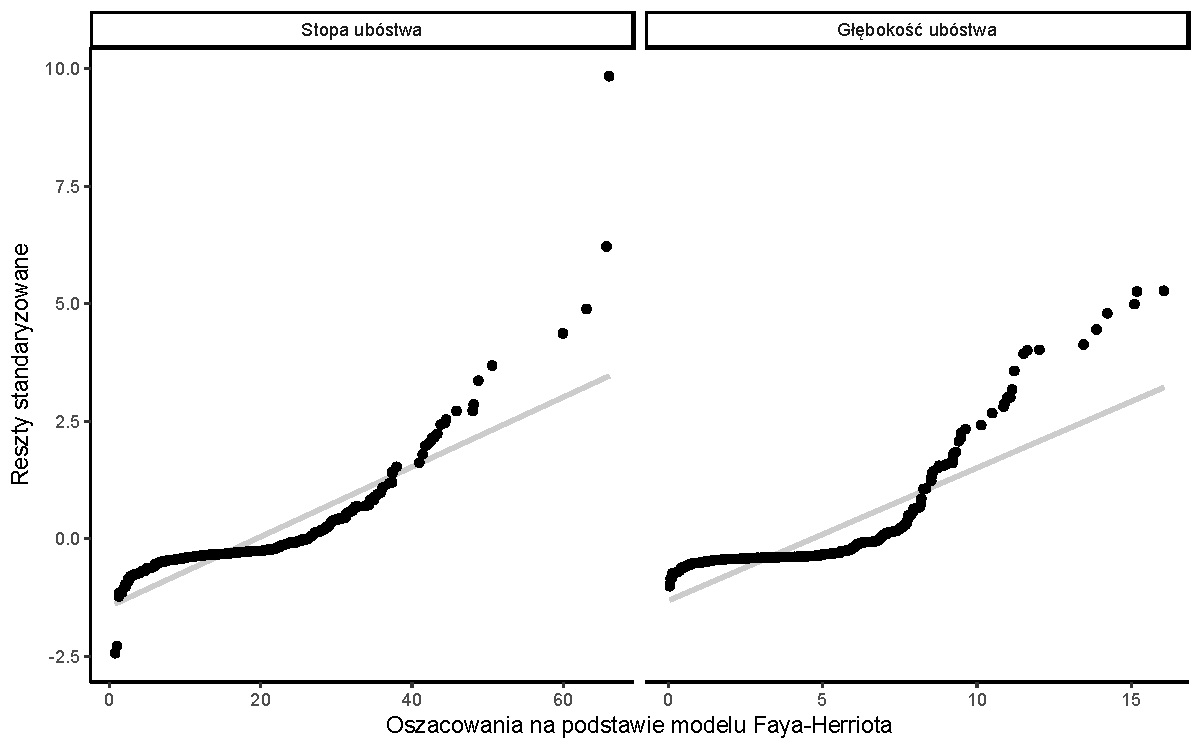
\includegraphics[width=0.8\textwidth]{04_wykresy/fh_pow_r_model-1.pdf}
\caption{Porównanie reszt standaryzowanych i oszacowań stopy oraz głębokości ubóstwa na poziomie powiatów}
\small{Źródło: opracowanie własne na podstawie badania EU-SILC 2011, NSP 2011 oraz BDL.}
\label{fig:fh_pow_r}
\end{figure}

Rozkład reszt dla obu wskaźników wyraźnie odbiega od rozkładu normalnego. Szczególnie duże wartości reszt są związane z wysokimi wartościami oszacowań. Liczba obserwacji w przypadku stopy ubóstwa, dla których reszta standaryzowana przekraczała wartość 3 było 11, natomiast dla głębokości ubóstwa takich powiatów było 12. W teście Kołmogorowa-Smirnowa odrzucono hipotezę zerową o zgodności rozkładów reszt z rozkładem normalnym.

Następnie zweryfikowano hipotezę o normalności efektów losowych porównując standaryzowane wartości z kwantylami rozkładu normalnego (por. rys. \ref{fig:fh_pow_u}).

\begin{figure}[htp]
\centering
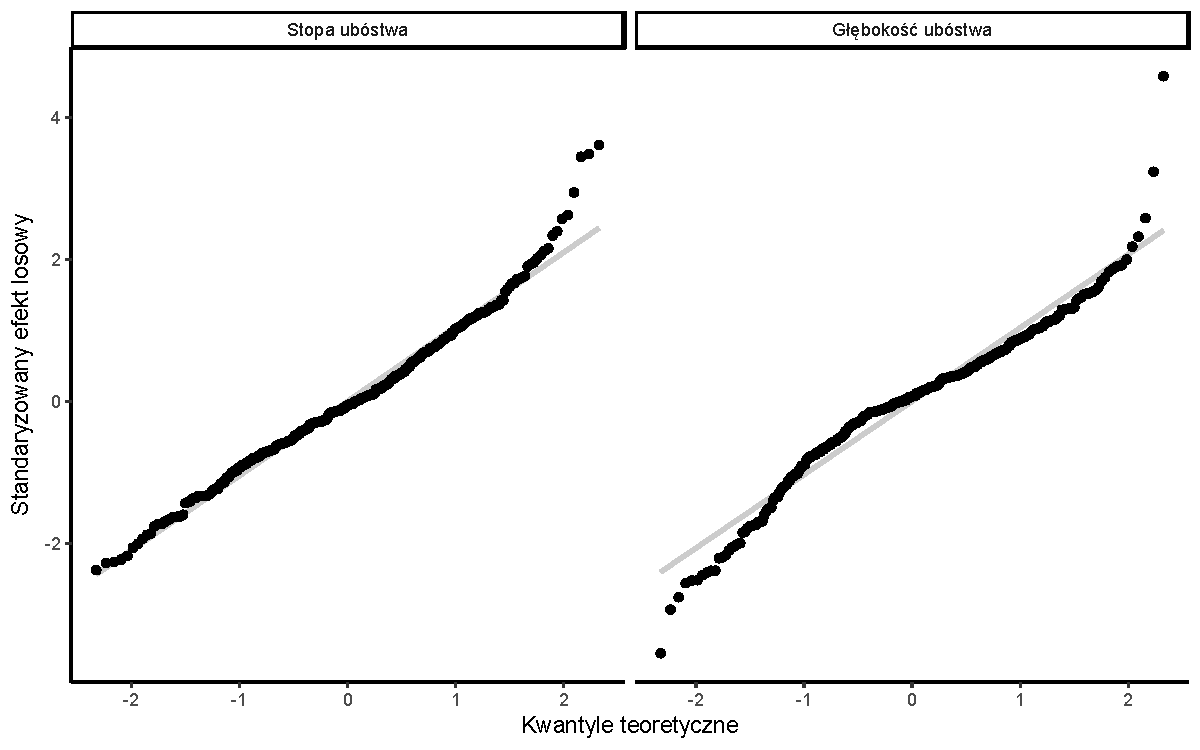
\includegraphics[width=0.8\textwidth]{04_wykresy/fh_pow_u_model-1.pdf}
\caption{Porównanie kwantyli efektów losowych i kwantyli rozkładu normalnego stopy oraz głębokości ubóstwa na poziomie powiatów}
\small{Źródło: opracowanie własne na podstawie badania EU-SILC 2011, NSP 2011 oraz BDL.}
\label{fig:fh_pow_u}
\end{figure}

Efekty losowe na poziomie powiatów dla stopy i głębokości ubóstwa mają rozkład normalny. Największą wartość odstającą odnotowano dla powiatu ełckiego. W obu przypadkach nie ma podstaw do odrzucenia hipotezy zerowej w teście Kołmogorowa-Smirnowa --- wartość p jest równa 0,5798 dla stopy ubóstwa, natomiast dla wskaźnika głębokości ubóstwa $p=0,0835$.

W tabeli \ref{tab:fh_pow_prec} przedstawiono odsetek powiatów należących do przedziału klasowego obejmującego określone wartości względnego błędu oszacowania stopy oraz głębokości ubóstwa uzyskane z wykorzystaniem estymatora bezpośredniego Horvitza-Thomsona oraz pośredniego SEBLUP.

\begin{table}[htp]
\caption{Porównanie precyzji oszacowań bezpośrednich oraz pośrednich stopy oraz głębokości ubóstwa na poziomie powiatów --- podejście obszarowe}
\label{tab:fh_pow_prec}
\centering
\begin{tabular}{lrrrr}
\hline
Wartość RRMSE & $F_0$ HT & $F_0$ SEBLUP & $F_1$ HT & $F_1$ SEBLUP\tabularnewline
\hline
{[}0\%--10\%{]} & 7 & 6 & 0 & 0 \\
(10\%--20\%{]} & 97 & 115 & 46 & 54 \\
(20\%--30\%{]} & 119 & 145 & 129 & 150 \\
(30\%--40\%{]} & 70 & 60 & 93 & 92 \\
powyżej 40\% & 71 & 53 & 96 & 83 \\
\hline
\end{tabular}\\
\small{Źródło: opracowanie własne na podstawie badania EU-SILC 2011, NSP 2011 oraz BDL.}
\end{table}

Niespełnienie wszystkich założeń modelu, występowanie wartości odstających oraz wysokie wartości oszacowań wariancji w podejściu bezpośrednim miały wpływ na fakt, że poprawa precyzji oszacowań pośrednich jest niewielka. Nastąpił wzrost frakcji powiatów znajdujących się w~przedziale od 10 do 20 procent wartości względnego błędu szacunku --- w przypadku stopy ubóstwa z 97 powiatów do 115 jednostek, a dla głębokości ubóstwa o 8 powiatów na korzyść estymacji pośredniej. Największa zmiana liczby powiatów obserwowana jest w przedziale 20\%-30\% wskaźnika precyzji. Pomimo zauważalnych zmian, dla stopy ubóstwa w dalszym ciągu w ponad 100 powiatach obserwuje się wartości względnego błędu oszacowania przekraczającego 30\%. 

\subsubsection{Modelowanie dochodu na poziomie gospodarstwa domowego}

Estymacja z wykorzystaniem modeli na poziomie obszaru w przekroju powiatów nie przyniosła oczekiwanej poprawy jakości oszacowań. Przy takiej liczbie jednostek i dużym zróżnicowaniu zmiennych zależnych estymatory obszarowe nie są w stanie zapewnić odpowiedniego poziomu precyzji. W związku z tym wykorzystano modele na poziomie jednostki.

Modele jednostkowe z kolei bazują na modelowaniu dochodów lub wydatków gospodarstw domowych z wykorzystaniem danych jednostkowych pochodzących z badań pełnych lub zasobów administracyjnych. W tym przypadku dostępność zmiennych niezależnych jest dużo mniejsza od tej występującej dla modeli obszarowych \citep{molina2016}. Dochód gospodarstwa domowego jest objaśniany przez charakterystyki tego gospodarstwa takie jak liczba osób bezrobotnych czy wskaźnik obciążenia demograficznego. Do najważniejszych technik estymacji opartych na modelach jednostkowych należą metody ELL \citep{ell2003}, MQ \citep{mq2006} oraz EB \citep{ebp2010}. Estymacja danego wskaźnika ubóstwa w przypadku tych metod polega na tworzeniu, z wykorzystaniem symulacji Monte Carlo, pseudo-populacji, które stanowią podstawę estymacji wskaźników ubóstwa. Wymienione metody są do siebie bardzo podobne jeśli chodzi o ideę, natomiast można wyróżnić kilka zasadniczych różnic. Metoda ELL nie uwzględnia w ogóle danych pochodzących z badania reprezentacyjnego, w przeciwieństwie do metody EB. Z~kolei metoda MQ jest odporna na obserwacje odstające.

Zastosowanie wyżej przedstawionych metod wymaga opracowania modelu opisującego dochód w gospodarstwach domowych. Jako zmienne pomocnicze wykorzystano cechy demograficzne, ekonomiczne, społeczne oraz terytorialne mierzone na poziomie gospodarstwa. Ponadto, dodano trzy cechy dostępne na poziomie powiatu. W końcowym modelu znalazły się następujące zmienne:

\begin{itemize}
\item poziom gospodarstwa
\begin{itemize}
\item odsetek mężczyzn w gospodarstwie,
\item odsetek osób w wieku 30-44 w gospodarstwie,
\item odsetek osób w wieku 65 lat i więcej w gospodarstwie,
\item odsetek osób bezrobotnych w gospodarstwie,
\item odsetek osób niepełnosprawnych w gospodarstwie,
\item odsetek osób z wykształceniem podstawowym w gospodarstwie,
\item odsetek osób z wykształceniem wyższym w gospodarstwie,
\item wskaźnik obciążenia demograficznego dzieci w gospodarstwie,
\item zmienna binarna - gospodarstwo posiada 1 pokój,
\item zmienna binarna - gospodarstwo posiada 3 pokoje i więcej,
\item zmienna binarna - miejsce zamieszkania: wieś lub miasto do 20 tys. osób,
\end{itemize}
\item poziom powiatu
\begin{itemize}
\item stopa bezrobocia rejestrowanego,
\item odsetek osób zatrudnionych w rolnictwie,
\item wypłacone świadczenie społeczne na 1000 zatrudnionych osób.
\end{itemize}
\end{itemize}

Dla tak określonego zestawu cech oszacowano liniowy model z efektem losowym na poziomie powiatu, w których zmienną zależną był ekwiwalentny dochód gospodarstwa. Model ten będzie określany mianem modelu dwupoziomowego, ze względu na losowy efekt powiatu oraz gospodarstwa domowego.

W tabeli \ref{tab:jedn_beta} przedstawiono parametry $\beta$ oraz oszacowane wariancje efektów losowych.

\begin{table}[htp]
\centering
\caption{Parametry $\beta$ modelu objaśniającego dochód ekwiwalentny na poziomie gospodarstwa domowego}
\label{tab:jedn_beta}
\begin{tabular}{p{10cm}rrr}
\hline
Zmienna niezależna & $\beta$ & błąd stand. & wartość p \\
\hline
wyraz wolny & 24916.24 & 579.64 & 0.0000 \\
odsetek mężczyzn w gospodarstwie & 3233.45 & 474.16 & 0.0000 \\
odsetek osób w wieku 30-44 w gospodarstwie & 1863.55 & 562.68 & 0.0009 \\
odsetek osób w wieku 65 lat i więcej w gospodarstwie & -2959.38 & 382.68 & 0.0000 \\
odsetek osób bezrobotnych w gospodarstwie & -15231.93 & 876.78 & 0.0000 \\
odsetek osób niepełnosprawnych w gospodarstwie & -8649.52 & 745.19 & 0.0000 \\
odsetek osób z wykształceniem podstawowym w gospodarstwie & -2534.25 & 448.32 & 0.0000 \\
odsetek osób z wykształceniem wyższym w gospodarstwie & 19061.33 & 486.28 & 0.0000 \\
wskaźnik obciążenia demograficznego dzieci w gospodarstwie & -3587.74 & 336.20 & 0.0000 \\
gospodarstwo posiada 1 pokój (zmienna binarna) & -2243.68 & 442.58 & 0.0000 \\
gospodarstwo posiada 3 pokoje i więcej (zmienna binarna) & 2824.66 & 272.51 & 0.0000 \\
miejsce zamieszkania: wieś lub miasto do 20 tys. (zmienna binarna) & -2857.61 & 321.58 & 0.0000 \\
\hline
stopa bezrobocia rejestrowanego & -10206.26 & 2632.61 & 0.0001 \\
odsetek osób zatrudnionych w rolnictwie & -8089.02 & 960.84 & 0.0000 \\
wypłacone świadczenie społeczne na 1000 zatrudnionych osób & -1597.30 & 374.01 & 0.0000 \\
\hline
$\sigma_u^2=1388,60$ & & & \\
$\sigma_e^2=13720,70$ & & & \\
\hline
\end{tabular}\\
\small{Źródło: opracowanie własne na podstawie badania EU-SILC 2011, NSP 2011 oraz BDL.}
\end{table}

Wszystkie zmienne niezależne są istotne i mają prawidłowy znak przy parametrze $\beta$. Wyższe wartości czterech zmiennych: odsetek mężczyzn w gospodarstwie, odsetek osób w wieku 30-44 w gospodarstwie, odsetek osób z wykształceniem wyższym w gospodarstwie oraz gospodarstwo posiada 3 pokoje i więcej (zmienna binarna) wpływają także na wzrost dochodu w gospodarstwie. Z kolei parametry przy pozostałych zmiennych mają ujemny znak co oznacza, że wyższe wartości tych cech powodują spadek dochodu w gospodarstwie. Trzy cechy mierzone na poziomie powiatów pokazują wpływ sytuacji ekonomicznej w danym obszarze na dochód pojedynczego gospodarstwa. Wyższa stopa bezrobocia, odsetek osób utrzymujących się z rolnictwa czy wyższy wskaźnik wypłacanych świadczeń z pomocy społecznej negatywnie wpływają na wysokość dochodu gospodarstwa.

%Następnie zweryfikowano normalność reszt oraz efektów losowych w modelu.
%
%\begin{figure}[htp]
%\includegraphics[width=\textwidth]{04_wykresy/doch_norm_lvl1-1.pdf}
%\caption{Porównanie reszt standaryzowanych oraz efektów losowych z kwantylami rozkładu normalnego}
%\small{Źródło: opracowanie własne na podstawie badania EU-SILC 2011, NSP 2011 oraz BDL.}
%\label{fig:doch_norm_lvl1}
%\end{figure}
%
%Wartości na wykresach wskazują, że nie zostały spełnione założenia dotyczące normalności rozkładu. Potwierdza to także przeprowadzony test Kołmogorowa-Smirnowa. Rozkład cechy na poziomie gospodarstwa jest zaburzony przez wcześniej zidentyfikowane wartości odstające - maksymalna wartość reszty standaryzowanej wynosi 37. Obserwacje przekraczające wartość 3 reszt standaryzowanych stanowią tylko 1,17\%. Z kolei na poziomie powiatów odnotowano 3 wartości odstające - m. st. Warszawa, powiat krapkowicki (opolskie) oraz złotoryjski (dolnośląskie). Podobnie na poziomie gmin - wysokie wartości dochodów determinują wielkość efektu losowego na tym poziomie.

W dalszej części pracy wykorzystano model przedstawiony w tabeli \ref{tab:jedn_beta} do estymacji stopy oraz głębokości ubóstwa na poziomie powiatów. W przypadku metody EB zastosowano przekształcenie zmiennej zależnej mające na celu spełnienie założeń o normalności. W metodzie MQ wykorzystano oryginalne wartości ze względu na odporny charakter tego podejścia.

\subsubsection{Estymacja pośrednia stopy oraz głębokości ubóstwa z wykorzystaniem podejścia jednostkowego}

Jak wskazano w podrozdziale \ref{pr:struktura-zmiennych}, rozkład dochodów ekwiwalentnych wyznaczony na podstawie badania EU-SILC charakteryzuje się silną asymetrią prawostronną, co może utrudnić proces modelowania. W celu poprawy własności takiego wektora stosuje się transformacje mające na celu zbliżenie rozkładu cechy do rozkładu normalnego. Do najczęściej stosowanych należy logarytmowanie, logarytmowanie z przesunięciem oraz przekształcenie Boxa-Coxa. W tej części pracy przeanalizowano wszystkie trzy możliwości w celu wyboru transformacji charakteryzującej się najlepszymi własnościami. 

W związku z występowaniem ujemnych wartości dochodu nie jest możliwe bezpośrednie zastosowanie transformacji logarytmicznej. Konieczne jest ustalenie wartości, którą należy dodać do dochodu każdego gospodarstwa, tak aby otrzymany wektor był dodatni. Minimalna wartość dochodu wynosi -7 800 zł, w związku z czym dochód każdego gospodarstwa zostanie powiększony o 7 801 zł, a następnie zlogarytmowany.

Celem transformacji logarytmicznej z przesunięciem jest ustalenie takiej wartości dochodu dodawanej do każdego gospodarstwa, aby rozkład cechy był symetryczny. Wartość tego parametru ustala się w sposób iteracyjny. Zmienna transformowana będzie symetryczna przy wartości przesunięcia równej 7 821,09 zł.

Następnie zastosowano transformację Boxa-Coxa. W tym celu użyto funkcję \emph{BoxCoxTrans} z~pakietu \emph{caret} \citep{caret2016} w programie R. Wykorzystuje ona logarytm wiarygodności do określenia optymalnej wartości parametru $\lambda$. Przeprowadzone obliczenia pozwoliły ustalić wartość parametru na poziomie $\lambda=0,1$.

W tabeli \ref{tab:trans} przedstawiono statystyki opisowe poszczególnych wektorów dochodu w zależności od przyjętego przekształcenia oraz wartości $\lambda$. Ponadto oszacowano model liniowy z wykorzystaniem wcześniej scharakteryzowanych zmiennych niezależnych, w związku z czym w tabeli znajdują się także wartości współczynnika $R^2$.

\begin{table}[htp]
\caption{Statystyki opisowe oraz wartość współczynnika determinacji w zależności od zastosowanej transformacji}
\label{tab:trans}
\centering
\begin{tabular}{lrrrrr}
\hline
Transformacja & $V_s$ & $\alpha_3$ & $\alpha_4$ & $R^2$ & $\lambda$\tabularnewline
\hline
Brak & 71,04 & 6,23 & 117,26 & 25,25 & - \tabularnewline
Logarytm & 4,07 & -0,76 & 30,44 & 30,65 & 7801,00 \tabularnewline
Logarytm z przesunięciem & 4,02 & 0,00 & 9,40 & 31,41 & 7821,09 \tabularnewline
Box-Cox & 6,47 & 0,37 & 6,81 & 31,72 & 0,10 \tabularnewline
\hline
\end{tabular}\\
\small{Źródło: opracowanie własne na podstawie badania EU-SILC 2011.}
\end{table}

Zastosowanie przedstawionych transformacji zmiennych zmniejszyło dyspersję, skośność oraz kurtozę ekwiwalentnego dochodu gospodarstw domowych. Współczynnik zmienności jest najniższy w przypadku transformacji logarytmicznej z przesunięciem. Ponadto rozkład cechy jest w tym przypadku symetryczny. Z kolei kurtoza jest najmniejsza przy przekształceniu Boxa-Coxa. Zastosowanie transformacji zmiennej wpłynęło na wzrost współczynnika determinacji o co najmniej 5 punktów procentowych. Najwyższym współczynnikiem $R^2$ charakteryzuje się model, uwzględniający transformację Boxa-Coxa. W związku z tym takie przekształcenie zastosowano w dalszej analizie.

Wykorzystując dane przedstawione na rysunku \ref{fig:bxcx_norm_lvl1} zweryfikowano normalność reszt oraz efektów losowych w modelu.

\begin{figure}[htp]
\centering
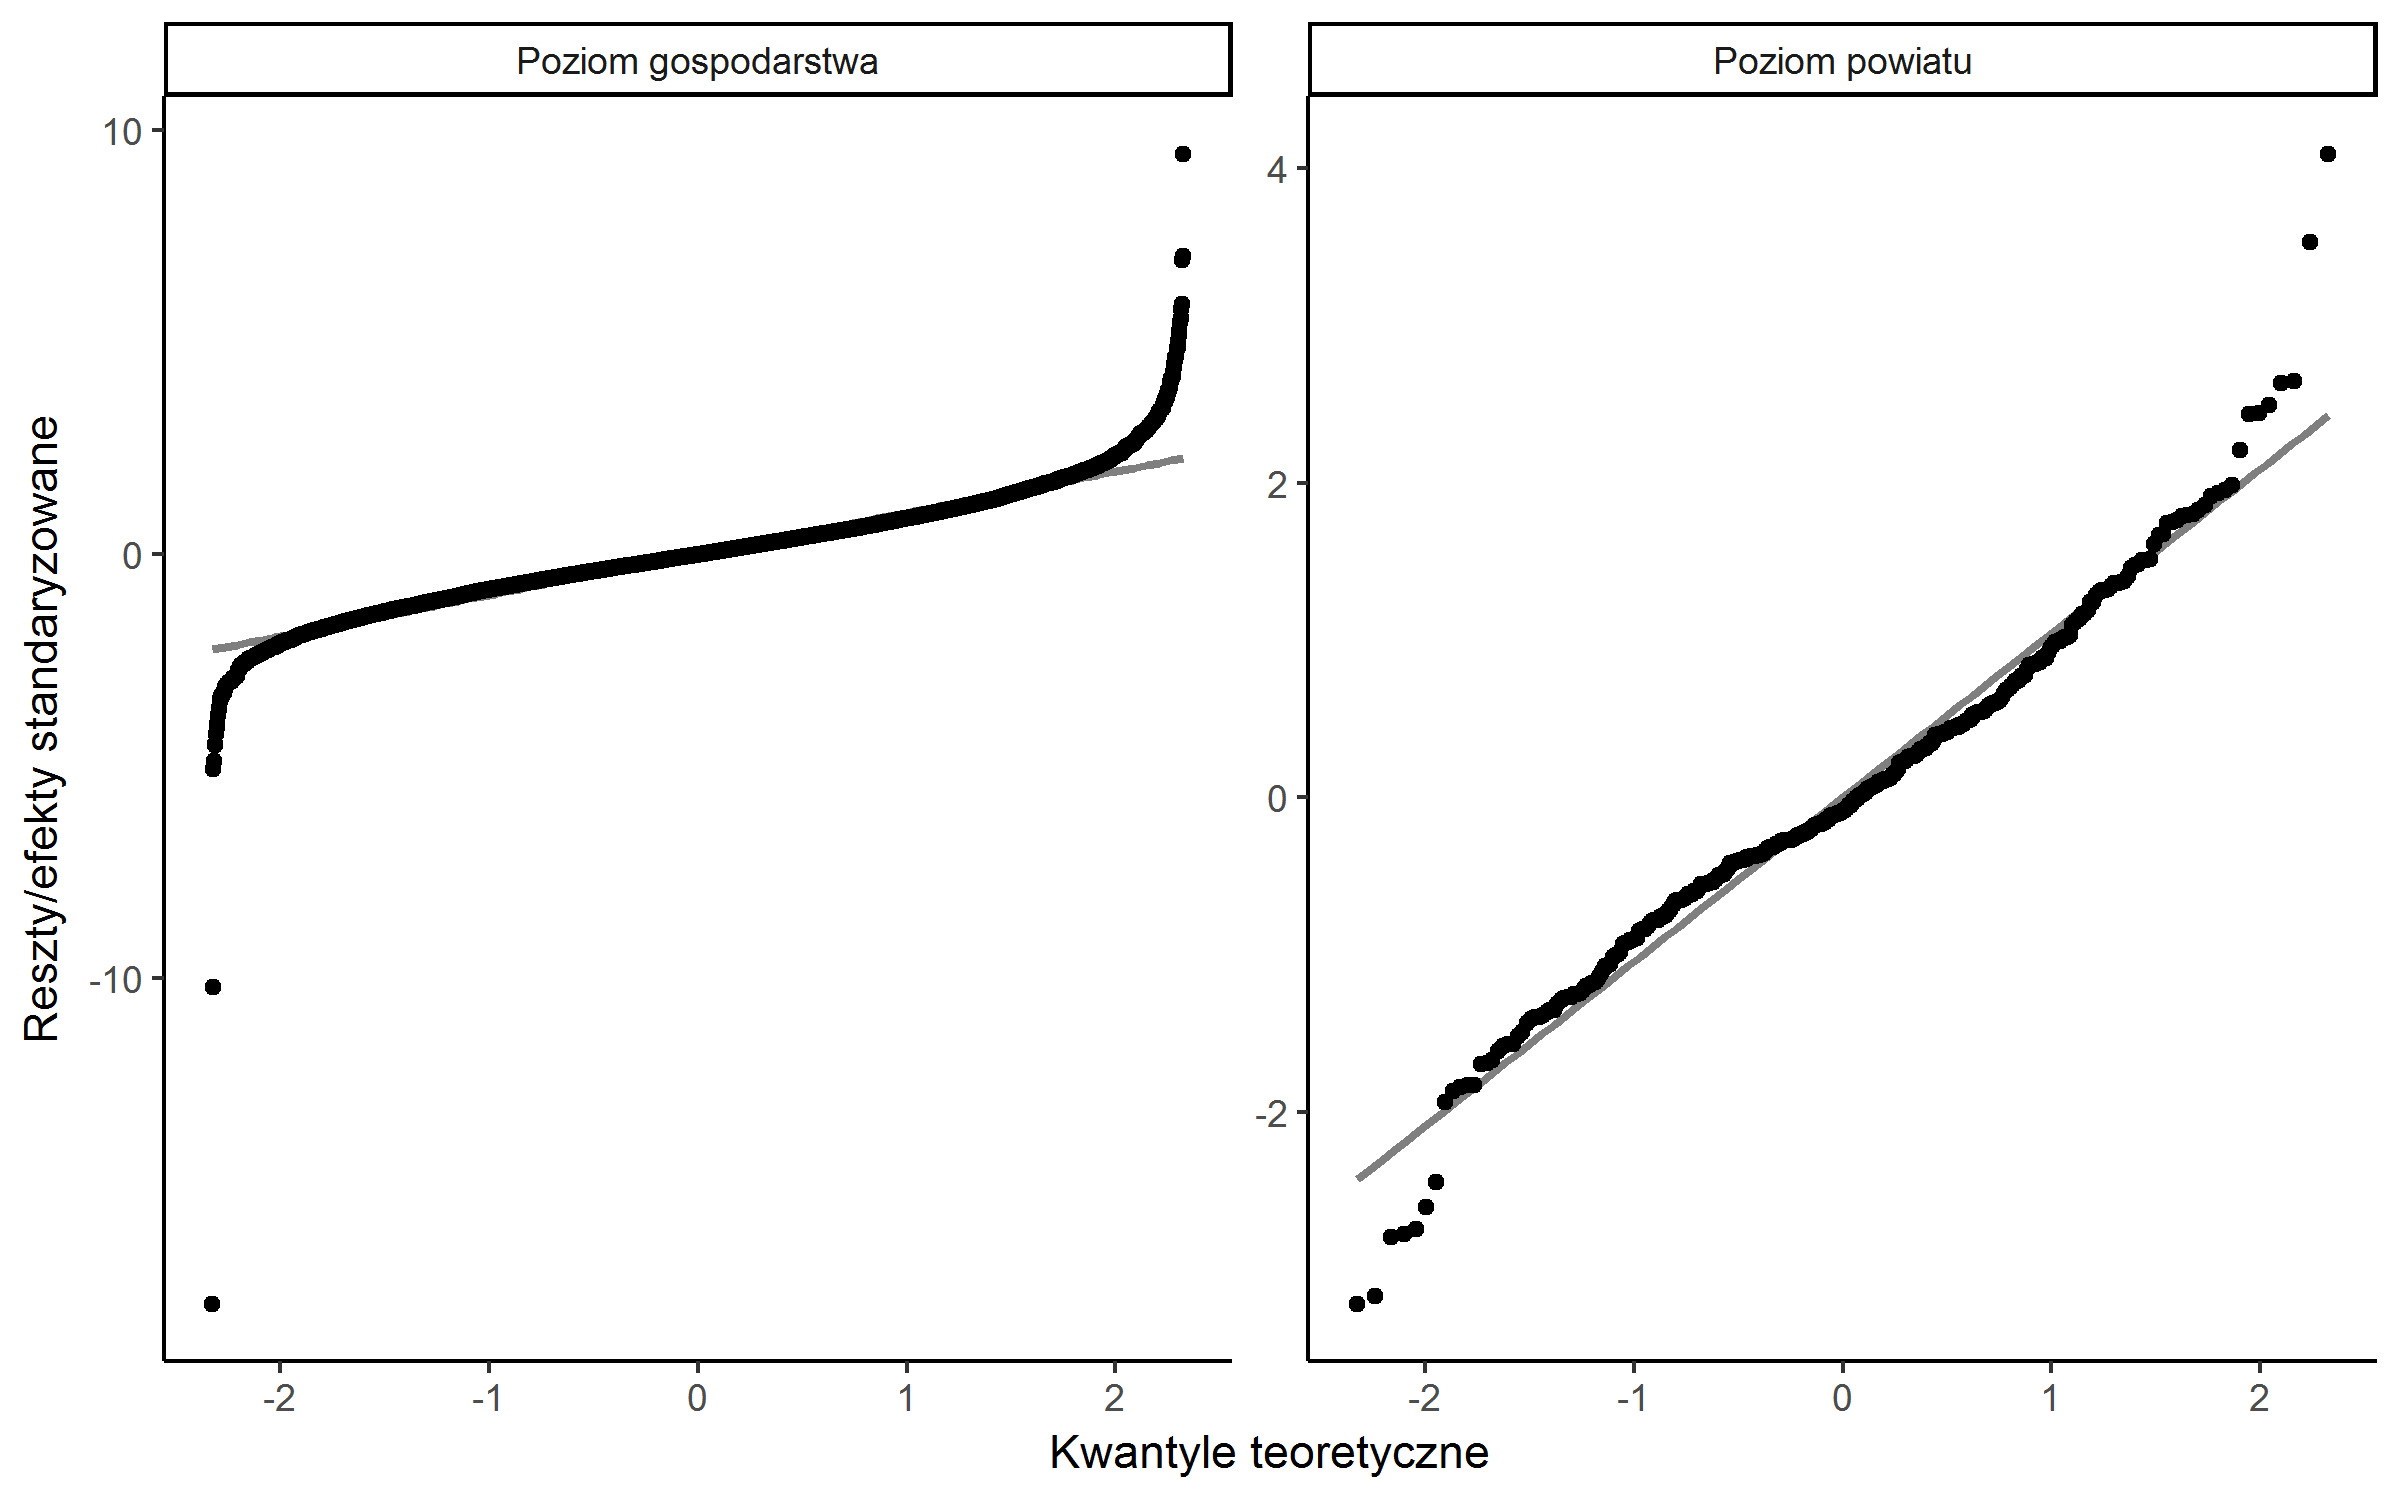
\includegraphics[width=0.8\textwidth]{04_wykresy/bxcx_norm_lvl1-1.png}
\caption{Porównanie reszt standaryzowanych i efektów losowych z kwantylami rozkładu normalnego --- transformacja Boxa-Coxa}
\small{Źródło: opracowanie własne na podstawie badania EU-SILC 2011, NSP 2011 oraz BDL.}
\label{fig:bxcx_norm_lvl1}
\end{figure}

Do najbardziej wpływowych obserwacji na poziomie gospodarstwa należy zaliczyć dwa gospodarstwa o bardzo niskich dochodach, położonych w powiecie świeckim (województwo kujawsko-pomorskie) oraz w m. Katowice. Na poziomie powiatów tylko jedna obserwacja przekracza wartość czterech efektów standaryzowanych --- powiat żuromiński w województwie mazowieckim. Z~wykorzystaniem testu Kołmogorowa-Smirnowa zweryfikowano hipotezę o normalności reszt oraz efektów losowych. Uzyskane reszty na poziomie gospodarstwa nie są zgodne z rozkładem normalnym. Z kolei w przypadku efektów losowych na poziomie powiatu w teście KS nie ma podstaw do odrzucenia hipotezy zerowej - wartość p w modelu dwupoziomowym wynosi 0,8357. Warunkowe kryterium informacyjne AIC \citep{caic2014} dla modelu liniowego z efektem losowym powiatu wynosi 35 257,00 i jest niższe w porównaniu do kryterium AIC policzonego dla zwykłego modelu liniowego: 35 323,13. Stanowi to przesłankę do dalszego stosowania tego typu modelowania.

Na rysunku \ref{fig:eb_mq_lvl1} przedstawiono oszacowania bezpośrednie oraz te uzyskane z zastosowaniem podejścia EB oraz MQ.

\begin{figure}[htp]
\centering
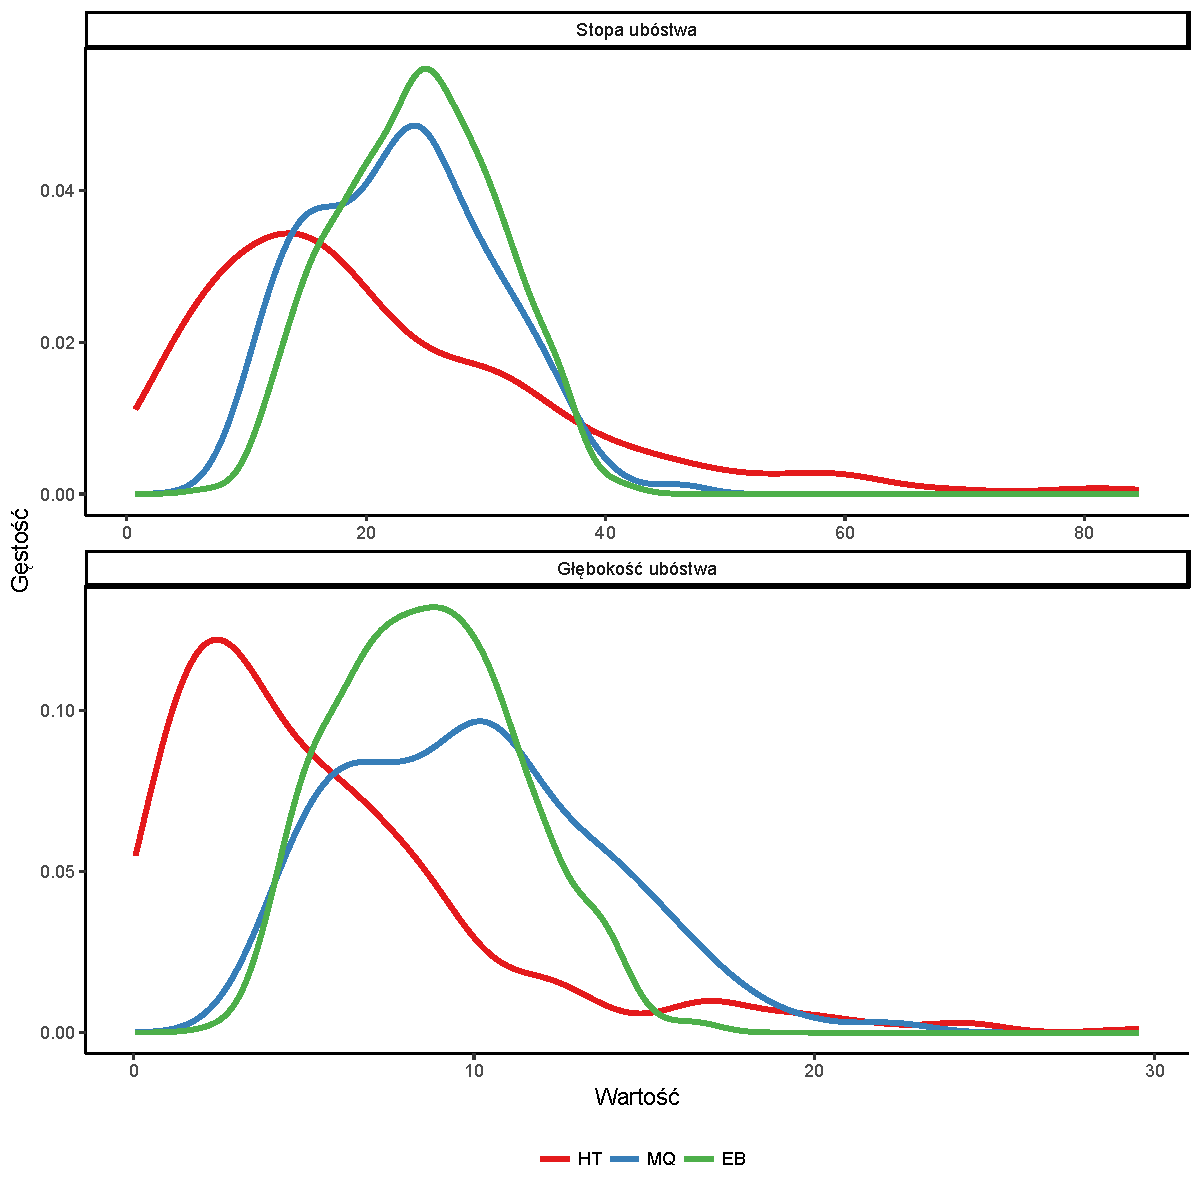
\includegraphics[width=0.8\textwidth]{04_wykresy/eb_mq_lvl1-1.pdf}
\caption{Rozkład oszacowań bezpośrednich oraz pośrednich stopy oraz głębokości ubóstwa na poziomie powiatów}
\small{Źródło: opracowanie własne na podstawie badania EU-SILC 2011, NSP 2011 oraz BDL.}
\label{fig:eb_mq_lvl1}
\end{figure}


Na rysunku można zaobserwować, że oszacowania uzyskane metodami pośrednimi są do siebie podobne, natomiast rozkłady bezpośrednich wskaźników ubóstwa od nich odbiegają. Średnia i mediana oszacowań stopy ubóstwa metodą MQ wynosi 23\%, a w przypadku metody EB 24,4\% i 24,5\% --- wartości te są bardzo zbliżone. Oszacowania bezpośrednie charakteryzują się średnią równą 20,8\% i medianą na poziomie 16,9\%. Ponadto trzeci moment centralny oszacowań EB jest równy 0. Obserwuje się także zmniejszenie rozstępu oszacowań stopy ubóstwa. W podejściu bezpośrednim wartości znajdowały się w przedziale {[}0,7\%--84,5\%{]}, natomiast po zastosowaniu podejścia jednostkowego oszacowania MQ mieszczą się w przedziale {[}6,8\%-46,7\%{]} oraz {[}6,9\%--41,1\%{]} dla metody EB. Podobne obserwacje można poczynić dla wskaźnika głębokości ubóstwa --- mediana oszacowań bezpośrednich wynosi 4,4\%, a dla podejścia MQ 9,9\% oraz 8,6\% dla EB. Rozstęp wskaźnika oszacowanego w sposób bezpośredni wynosi 29,5 punktów procentowych, 20 p.p.~dla oszacowań M-kwantylowych i 14 p.p.~dla oszacowań EB. Estymacja pośrednia wyeliminowała ekstremalnie niskie i wysokie wartości, które w rzeczywistości byłyby raczej nieobserwowane. Zastosowane podejście umożliwiło także estymację dla domen, dla których nie można było zastosować estymatora bezpośredniego.

\subsubsection{Ocena precyzji}

Na rysunku \ref{fig:eb_mq_lvl1_prec} porównano precyzję oszacowań bezpośrednich oraz uzyskanych metodą EB i~MQ.

\begin{figure}[htp]
\centering
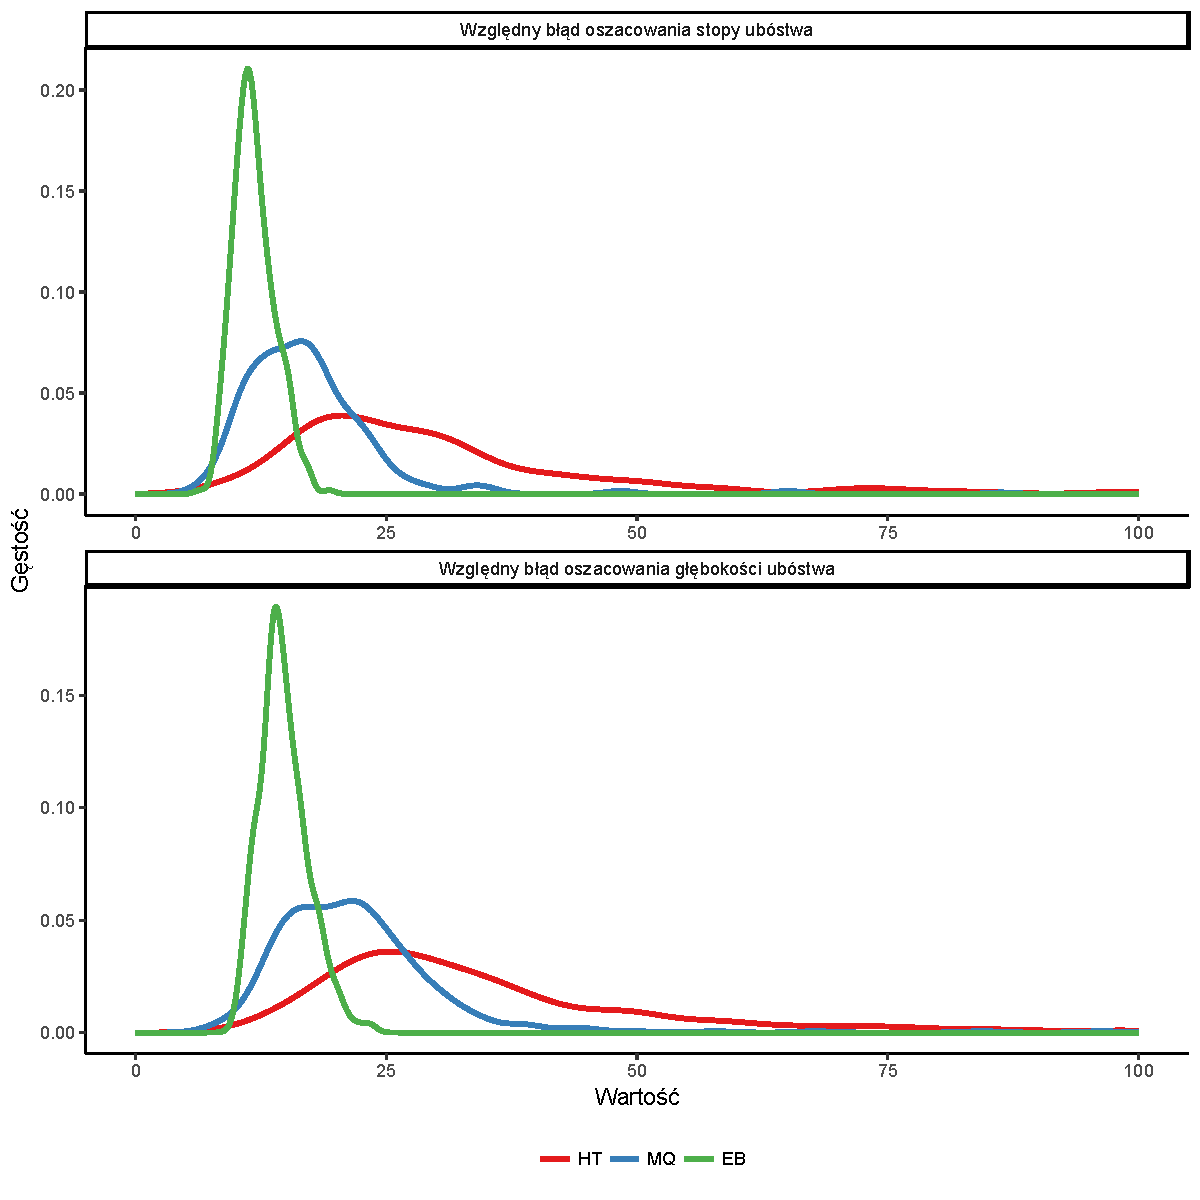
\includegraphics[width=0.8\textwidth]{04_wykresy/eb_mq_lvl1_prec-1.pdf}
\caption{Rozkład względnych błędów oszacowań bezpośrednich oraz pośrednich stopy oraz głębokości ubóstwa na poziomie powiatów}
\small{Źródło: opracowanie własne na podstawie badania EU-SILC 2011, NSP 2011 oraz BDL.}
\label{fig:eb_mq_lvl1_prec}
\end{figure}

Dane przedstawione na rysunku pokazują, że najniższymi wartościami względnych błędów oszacowań charakteryzuje się podejście EB. Rozkład wartości jest leptokurtyczny. Mediana wskaźnika precyzji dla oszacowań bezpośrednich stopy ubóstwa wynosiła 25,9\%, a zastosowanie estymacji pośredniej pozwoliło na obniżenie tej wartości do 16,3\% (MQ) i 11,6\% (EB). Także w~przypadku głębokości ubóstwa zauważalna jest poprawa --- wartość środkowa względnego błędu oszacowań wynosi 14,5\% dla metody EB, 21\% w podejściu MQ oraz 30,3\% stosując estymację bezpośrednią. Największy zysk na precyzji obserwowany jest w przypadku metody EB. 

\subsubsection{Ocena obciążenia}

Z wykorzystaniem testu Walda sprawdzono także istotność różnic pomiędzy oszacowaniami pośrednimi oraz bezpośrednimi. Wyniki przedstawiono w tabeli \ref{tab:wald_pow_eb}.

\begin{table}[htp]
\caption{Wartości statystyki Walda dla oszacowań pośrednich stopy oraz głębokości ubóstwa na poziomie powiatów --- podejście jednostkowe}
\label{tab:wald_pow_eb}
\centering
\begin{tabular}{lrr}
\hline
Estymator & Stopa ubóstwa & Głębokość ubóstwa\tabularnewline
\hline
EB & 2505,89 & 3652,39\tabularnewline
MQ & 1514,17 & 2523,84\tabularnewline
$\chi^2_{364}$ & \multicolumn{2}{c}{409,49} \tabularnewline
\hline
\end{tabular}\\
\small{Źródło: opracowanie własne na podstawie badania EU-SILC 2011, NSP 2011
oraz BDL.}
\end{table}

Oszacowania wskaźników ubóstwa uzyskane z wykorzystaniem metod EB oraz MQ istotnie różnią się od oszacowań bezpośrednich. Taki stan rzeczy wynika z dwóch faktów. Po pierwsze, wykorzystana metoda oceny obciążenia dedykowana jest podejściu obszarowemu. Po drugie, w~estymacji z wykorzystaniem wyżej wymienionych metod jednostkowych nie korzysta się z bezpośrednich oszacowań wskaźników ubóstwa.

Przeprowadzono także test pokrycia dla stopy ubóstwa, w którym 210 oszacowań EB oraz 240 oszacowań MQ znalazło się w 95\% przedziale ufności, co skutkuje odrzuceniem hipotezy zerowej mówiącej o pokryciu rzędu 95\%. W przypadku stopy ubóstwa pokrywające się oszacowania stanowiły 58\% (EB) i 66\% (MQ) wszystkich oszacowań. Dla głębokości ubóstwa pokrycie to jest jeszcze mniejsze i wynosi 45\% dla metody EB i 48\% dla metody MQ.

W tabeli \ref{tab:jedn_prec} przedstawiono precyzję oszacowań w podziale na przedziały klasowe o rozpiętości 10 punktów procentowych.

\begin{table}[htp]
\caption{Porównanie precyzji oszacowań bezpośrednich oraz pośrednich stopy oraz głębokości ubóstwa na poziomie powiatów --- podejście jednostkowe}
\label{tab:jedn_prec}
\centering
\begin{tabular}{lrrrrrr}
\hline
Wartość RRMSE & $F_0$ HT & $F_0$ MQ & $F_0$ EB & $F_1$ HT & $F_1$ MQ & $F_1$ EB \tabularnewline
\hline
{[}0\%--10\%{]} & 0 & 26 & 69 & 0 & 6 & 1 \tabularnewline
(10\%--20\%{]} & 51 & 261 & 310 & 28 & 159 & 367 \tabularnewline
(20\%--30\%{]} & 148 & 75 & 0 & 128 & 168 & 11 \tabularnewline
(30\%--40\%{]} & 94 & 7 & 0 & 104 & 31 & 0 \tabularnewline
powyżej 40\% & 71 & 6 & 0 & 104 & 11 & 0 \tabularnewline
\hline
\end{tabular}\\
\small{Źródło: opracowanie własne na podstawie badania EU-SILC 2011, NSP 2011 oraz BDL.}
\end{table}

Estymacja pośrednia poprawia precyzję oszacowań w porównaniu do estymacji bezpośredniej. Zarówno w przypadku stopy, jak i głębokości ubóstwa największy zysk na precyzji w porównaniu do estymacji bezpośredniej obserwuje się w metodzie EB. Względny błąd oszacowania stopy ubóstwa nie przekracza 20\%. Precyzja oszacowań uzyskanych metodą MQ jest gorsza aniżeli w~podejściu EB, ale i tak zauważalna jest poprawa w odniesieniu do estymacji bezpośredniej.

\section{Podsumowanie}

W niniejszym rozdziale dokonano oceny jakości zmiennych dochodowych pochodzących z badania EU-SILC. Zweryfikowano zgodność dokumentacji badania ze stanem faktycznym, wskazując pojawiające się rozbieżności. Ocenie poddano także skalę stosowania imputacji oraz przeprowadzania wywiadu zastępczego. Stwierdzono, że w przypadku wielu zmiennych dochodowych dotyczących osób informacje pozyskane od respondentów stanowiły mniej niż 50\% wszystkich odpowiedzi --- w pozostałej części korzystano z częściowej lub całkowitej imputacji wartości dochodu. Wywiad zastępczy również przyczyniał się do wzrostu odsetka imputacji. Dużo lepsza była jakość dochodu mierzonego na poziomie gospodarstwa domowego --- w większości przypadków udało się pozyskać kompletną informację. Wyjątek stanowiła kategoria dotycząca dochodu z własności finansowej. Przeprowadzona analiza jakości pozwoliła stwierdzić, że badanie EU-SILC nie jest badaniem doskonałym i należy mieć świadomość czynników mających wpływ na jakość danych wykorzystywanych później do estymacji wskaźników ubóstwa.

% W kwestionariuszu badania EU-SILC jest dział oceniający wywiad indywidualny, gdzie znajduje się pytanie dotyczące korzystania przez respondenta z dokumentów podatkowych podczas odpowiadania na pytania związane z sytuacją dochodową. Niestety ta zmienna nie wchodzi w skład zbiorów wykorzystywanych w analizie. Możliwe, że jej wykorzystanie mogłoby udoskonalić przeprowadzoną analizę.

W drugiej części rozdziału dokonano estymacji stopy oraz głębokości ubóstwa na poziomie podregionów oraz powiatów. Punktem wyjścia prac na poziomie podregionów był model objaśniający stopę ubóstwa wypracowany przez GUS w ramach współpracy z Bankiem Światowym. W toku prowadzonych badań wypracowano alternatywny model wyjaśniający zmienność stopy ubóstwa oraz zidentyfikowano symptomy dobrze wyjaśniające zmienność głębokości ubóstwa. W~obliczeniach wykorzystano klasyczny model Faya-Herriota oraz wariant tego modelu uwzględniający skorelowane przestrzennie efekty losowe. W odniesieniu do zmiennej zależnej zastosowano transformację pierwiastkiem arcus sinusa, która miała na celu zapewnienie oszacowań z przedziału $[0;1]$ oraz ustabilizować wariancję oszacowań bezpośrednich. Przeprowadzona analiza wskazała, że zastosowanie takiego przekształcenia zmiennej zależnej powoduje znaczne obciążenie oszacowań. Spośród rozważanych metod, najlepszymi własnościami charakteryzował się estymator SEBLUP uwzględniający w estymacji autokorelację efektów losowych. Dzięki zastosowaniu metod pośrednich udało się uzyskać zadowalającą poprawę precyzji na poziomie podregionów w porównaniu do estymacji bezpośredniej, zarówno dla wskaźnika zasięgu ubóstwa, jak i głębokości ubóstwa.

Kolejnym etapem badań było opracowanie modelu dla poziomu powiatów. Z racji dużo większej liczby obszarów niż na poziomie podregionów, rozkład liczebności próby charakteryzował się dużym zróżnicowaniem. Skutkowało to bardzo dużymi oszacowaniami wariancji oraz ekstremalnymi ocenami wskaźników ubóstwa uzyskanymi za pomocą estymatora bezpośredniego. Ponadto dla 16 powiatów, zastosowanie klasycznego podejścia do estymacji nie było możliwe, ze względu na brak dostatecznej liczby reprezentantów badanego zjawiska. Na podstawie dostępnych danych opracowano dwa modele --- dla wskaźnika stopy oraz głębokości ubóstwa. Podobnie, jak w przypadku podregionów, także w tym przypadku zastosowano przekształcenie zmiennej zależnej. Otrzymane rezultaty wskazały, że na poziomie powiatów również występuje obciążenie oszacowań pośrednich wykorzystujących transformację pierwiastkiem arcus sinusa. Biorąc pod uwagę kryterium precyzji oraz obciążenia, za estymator cechujący się najlepszymi własnościami uznano estymator SEBLUP \citep{wawrowski2016}. Niemniej zastosowanie tego podejścia na poziomie powiatów nie przyczyniło się do znaczącej poprawy precyzji mierzonej przez względny błąd oszacowania. 

Wobec niezadowalającej precyzji oszacowań pośrednich uzyskanych z zastosowaniem podejścia obszarowego, podjęto próbę estymacji wskaźników ubóstwa wykorzystując podejście jednostkowe. Bazując na dostępnych danych pochodzących z badania EU-SILC oraz Narodowego Spisu Powszechnego Ludności i Mieszkań 2011 dopasowano model z efektem losowym na poziomie powiatów. W modelu opisującym ekwiwalentny dochód gospodarstwa znalazło się 14 zmiennych niezależnych, w tym 11 mierzonych na poziomie gospodarstwa domowego i 3 na poziomie powiatów. Wypracowany model zastosowano w dwóch metodach --- EB oraz MQ. W pierwszym z tych podejść rozważano różne transformacje zmiennej zależnej --- najlepsze wyniki uzyskano stosując przekształcenie Boxa-Coxa. Podejście MQ bazuje na nietransformowanych wartościach dochodu. Wyniki otrzymane z zastosowaniem tych metod były do siebie zbliżone, niemniej stosując kryterium najniższego względnego błędu oszacowania, najbardziej precyzyjne oceny wskaźników ubóstwa uzyskano z wykorzystaniem metody EB.